\documentclass[11pt,oneside,final]{huthesis}
\usepackage{url,graphicx,color,multirow,hyperref}
\hypersetup{
  bookmarks=true,
  unicode=true,
  pdftoolbar=true,
  pdfmenubar=true,
  pdffitwindow=true,
  pdfstartview={FitV},
  pdftitle={Data Fidelity and Resource Management for Data-Rich Sensor Networks}
  pdfauthor={Geoffrey Werner Challen},
  pdfnewwindow=true,
  colorlinks=false,
  pdfdisplaydoctitle=true,
  pdfborder={0 0 0}
}
\usepackage[all]{hypcap}

\pdfinfo{
   /Author (Geoffrey Werner Challen)
   /Title  (Data Fidelity and Resource Management for Data-Rich Sensor Networks)
}

\input{.xxxnote}

% 11 Jan 2010 : GWA : Maximum table of contents depth.
%               1 = section
%               2 = subsection
%               3 = subsubsection
\setcounter{tocdepth}{2}
\setlength{\parindent}{0.25in}

\begin{document}

% 11 Jan 2010 : GWA : Spacing: \ssp for draft mode, \dsp for GSAS
%               requirement.
%\input{.spacing}

% 11 Jan 2010 : GWA : Chapter content.

% 11 Jan 2010 : GWA : frontmatter includes the abstract, table of contents,
%               acknowledgments and dedication.

\chapter{Case Study: Volcano Monitoring}
\label{chapter-background}

\XXXnote{GWA: TODO: Need to rewrite this.}

Beginning in 2004, computer scientists from Harvard University joined forces
with seismologists from the University of New Hampshire, the University of
North Carolina, and Instituto Geof\'{i}sico, Escuela Polit\'{e}cnica
Nacional, Ecuador, to begin a collaboration aimed at using sensor networks to
further the study of active volcanoes. As of early 2009 our collaboration has
spanned three successful deployments, multiple scientific publications and
generated a large number of interesting ideas to explore.  We have been
fortunate to be a part of this long-running partnership.

From a simple starting point --- a handful of nodes streaming continuous data
from a single sensor per node --- we have developed a sophisticated
resource-aware architecture carefully balancing the value of the data to the
application against the network-wide cost of extraction. These design changes
were motivated by the science goals, responsive to changing hardware
platforms, and driven by experience gained deploying prior iterations.
Because each of the three deployments is already well-documented, one of our
goals is to illuminate the design process by linking successive artifacts
together while maintaining the thread of data quality as an application
driver.

From the beginning of our work, providing high quality data has remained a
part of our research agenda. This focus emerged out of both the scientific
goals, and constraints of the devices we have deployed. Because seismologists
are used to processing high-resolution data from multiple stations, wireless
sensor networks --- while considerable less burdensome than existing
instrumentation --- must provide data of similar quality before they can be
used for scientific study.  The scale made possible by rapid deployment
promised by augmenting existing seismological instrumentation with wireless
sensor network hardware is new, but the existence of data processing
techniques means that the requirements are already firmly in place.

Designing wireless sensor network applications in this space has required
work to meet some of the data quality requirements while finding ways of
creatively relaxing others.  Specifically, we have found it necessary to
deliver high-resolution data meeting strict timing requirements, but found
flexibility in terms of providing a complete data set from every node
covering all moments of time.

\section{Overview of Seismoacoustic Monitoring}

Volcanic monitoring has a wide range of goals, related to both scientific
studies and hazard monitoring. Figure~\ref{introduction-fig-cartoon} displays
an overview of several instruments that might be used, the signals that they
collect and example configurations used during deployments. The type and
configuration of the instrumentation depends on the goals of a particular
study.  Traditionally, dispersed networks of seismographs, which record
ground-propagating elastic energy, are utilized to locate, determine the size
of, and assess focal mechanisms (source motions) of earthquakes occurring
within a volcanic edifice~\cite{Chouet03}.  At least four
spatially-distributed seismographs are required to constrain hypocentral (3D)
source location and origin time of an earthquake, though using more seismic
elements enhances hypocenter resolution and the understanding of source
mechanisms. Understanding spatial and temporal changes in the character of
volcanic earthquakes is essential for tracking volcanic activity, as well as
predicting eruptions and paroxysmal events~\cite{McNutt96}. 

Another use of seismic networks is the imaging of the internal structure of a
volcano through tomographic inversion.  Earthquakes recorded by
spatially-distributed seismometers provide information about propagation
velocities between a particular source and receiver.  A seismically-active
volcano thus allows for three-dimensional imaging of the volcano's velocity
structure~\cite{Benz96,Phillips91}. The velocity structure can then be
related to material properties of the volcano, which may be used to determine
the existence of a magma chamber~\cite{Lees89,Moran99}.  Dense array
configurations, with as many as several dozen seismographs, are also an
important focus of volcanic research~\cite{Dietel89,Neuberg94}. Correlated
seismic body and surface wave phases can be tracked as they cross the array
elements, enabling particle motion and wavefield analysis, source
back-azimuth calculations, and enhanced signal-to-noise recovery.

\section{Opportunities for Wireless Sensor Networks}

\begin{figure}[t] 
\begin{center} 
\includegraphics[width=0.9\hsize,clip=true,bb=20 470 540 770]{./2-casestudy/figs/Cartoon2.pdf}
\end{center} 
\caption{\textbf{Sensor arrays for volcanic monitoring.}}
\label{introduction-fig-cartoon} 
\end{figure}

Networks of spatially-distributed sensors are commonly used to monitor
volcanic activity, both for hazard monitoring and scientific
research~\cite{Scarpa96}.  Typical types of sensing instruments include
seismic, acoustic, GPS, tilt-meter, optical thermal, and gas flux.  Volcanic
sensors range from widely dispersed instrument networks to more confined
sensor arrays. An individual sensor station could consist of a single sensor
(e.g., seismometer or tilt sensor), or an array of several closely-spaced
($10^2$ to $10^3$~m aperture) wired sensors, perhaps of different types.
Multiple stations may be integrated into a larger network installed over an
extended azimuthal distribution and radial distance ($10^2$ to $10^4$~m) from
the volcanic vent.  Data from various stations may be either recorded
continuously or as triggered events and the acquisition bandwidth depends
upon the specific data stream. For instance, seismic data is often acquired
at 24-bit resolution at 100~Hz, while tilt data may be recorded with 12-bit
resolution at 1~Hz or less.

Unfortunately, the number of deployed sensors at a given volcano is usually
limited by a variety of factors, including: monetary expenses such as sensor,
communication, and power costs; logistical concerns related to time and access
issues; and archival and telemetry bandwidth constraints. Due to their small
size, light weight, and relatively low cost, wireless sensor nodes have an
important role to play in augmenting and extending existing seismic
instrumentation, providing the increased spatial resolution necessary to
support seismic applications like tomography.

Sensor data at a station may be recorded locally or transmitted over
long-distance radio or telephone links to an observatory located tens of
kilometers from the volcano.  At the receiving site, data is displayed on
revolving paper helicorders for rapid general interpretation and
simultaneously digitized for further processing.  However, due to the expense
and bandwidth constraints of radio telemetry, high-quality, multi-channel
data acquisition at a particular volcano is often limited. These analog
systems also suffer from signal degradation and communication interference.

As a result, many scientific experiments use a stand-alone data acquisition
system at each recording station.  The digitizer performs high-resolution
analog-to-digital conversion from the wired sensors and stores data on a hard
drive or Compact Flash card. However, these systems are cumbersome, power
hungry ($\approx 10$~Watts), and require data to be manually retrieved from
the station prior to processing. Depending on the size of the recording
media, a station may record several days or weeks' worth of data before it
must be serviced. Deploying a wireless sensor network with telemetry to the
base station allows real time data collection, network monitoring and
retasking not possible with untelemetered systems.



\chapter{Introduction}
\label{chap-introduction}

Wireless sensor networks composed of tens or hundreds of low-power,
resource-constrained devices, can aid scientific exploration by providing
high-fidelity data at scales more difficult to achieve with traditional
instrumentation. In his book \textit{The Macroscope}, French futurist Joel de
Rosnay envisioned a new scientific instrument: the \textit{macroscope}. As a
large-scale analog to the microscope, the macroscope would be able to provide
insights into large systems that are difficult to study at scale: entire
cities, ecosystems, or planetary-scale systems.

Realizing the scientific macroscope using sensor network technology requires
confronting several core challenges. Data collected by the system must be
able to match the fidelity of signals collected from higher-power
instruments. When resource limitations limit the amount of data that can be
collected, the system should focus its limited energy or bandwidth on the
highest value signals. The network should continuously adapt to the resource
limitations inherent to sensor network technology and gracefully adjust as
energy and bandwidth availability fluctuate.

This dissertation presents the design of a scientific macroscope using
wireless sensor networks as an enabling technology, as well as two
architectural solutions designed to improve the sensor macroscope's
performance by managing distributed network resources. In this dissertation,
we first validate that data collected by wireless sensor nodes can meet the
needs of a demanding, high data-rate scientific application: volcano
monitoring. We then describe new sensor network architectures that improve
the data quality provided to the application by the sensor macroscope.
Together these techniques begin the process of realizing de Rosnay's vision
using embedded sensing.

\section{Scientific Sensor Networks}

\XXXnote{GWA: Need to fill this in.}

\section{Architectural Challenges}

Wireless sensor networks consist of nodes integrating modest amounts of
computation, storage, and communication capabilities. The use of low-power
microprocessors, radios, and MEMS sensors enables embedded sensing on power
budgets not feasible a decade ago.

Early sensor network researchers saw the potential for these new devices to
aid in scientific studies. One of the first published deployments of embedded
sensing technology was on Great Duck Island in Maine, where a network of 32
sensor nodes was used to study the nesting behavior of a colony of
Seabirds~\cite{gdi-sensys04}. Another early experiment used similar nodes to
study the microclimate of a single Redwood tree~\cite{berkeley-redwoods}.  In
contrast to these early efforts, our group has focused on \textit{high
data-rate} scientific applications. Compared with low data-rate monitoring,
these produce a distinct set of research challenges.

\begin{enumerate}

\item \textbf{Data fidelity.} High data-rates stress the ability of the
system to provide high fidelity data. Sampling at high rates introduces
additional load on each node, which can interfere with its participation in
routing, time synchronization, or data transfer protocols. Frequently, timing
accuracy requirements scale with the sampling rate, so that data sampled at
high rates must be assigned precise timestamps to facilitate comparisons
between multiple stations.

\textit{Problem Statement:}

\item \textbf{Optimizing overall data quality.} In addition, high sampling
rates challenge the ability of the system to achieve low-power operation.
Sampling, storing, and transmitting large amounts of data prevents nodes from
entering into low-power states and can consume a great deal of their stored
energy.  Once data rates and network sizes pass a certain point, all data
cannot be collected in real time, meaning that the system must choose what
data to discard and what to retrieve. Depending on the phenomena being
monitored, some data is likely to be interesting and some less interesting. A
habitat monitoring application may want to focus on collecting vocalizations
from a certain kind of animal. Differences in sensor quality may also lead to
data value disparities, when poorly-located or poorly-functioning sensors
sample data that is of poor quality and of little value to the application.

\textit{Problem Statement:}

\item \textbf{Network-wide energy disparities.} When energy-harvesting
technologies are deployed, variances in energy availability across the
network can challenge the ability of the entire system to achieve good
performance. Many sensor network protocols may concentrate energy usage on a
small set of nodes, leading to poor network performance if and when those
nodes batteries are exhausted. Enabling good performance of the network as a
whole requires adapting to variance in resource availability as it happens,
and adjusting network behavior in ways that allow nodes with large amounts of
energy to take on new roles and nodes with low batteries to reduce their
responsibilities.

\textit{Problem Statement:}

\end{enumerate}

When tackling these challenges, our approach has been inspired by our vision
of a set of sensor nodes functioning \textit{as a single instrument}. We have
tried to design architectures that abandon a node-level view in favor of this
network-level perspective. This challenges the way that many sensor network
protocols are designed, since they assume that greedy local decision making
will produce node behaviors that are beneficial for the entire system.
Instead, the two architectures described in this dissertation attempt to
connect local node behaviors with the resulting value of the entire
instrument to the intended scientific application.

\section{Dissertation Summary and Contributions}

This dissertation makes the following contributions:

\begin{itemize}

\item \textbf{Detailed evaluation of a scientific macroscope.} We have built
and fielded the first sensor network designed to study active volcanos. After
an initial pilot deployment, a system was designed giving careful
consideration to the scientific requirements. In total, we have performed
three deployments of iterations of our system at active volcanoes in Ecuador.
All three are summarized below:

\begin{enumerate}

\item \textbf{July, 2004, Tungurahua Volcano:} We deployed three infrasonic
monitoring nodes continuously transmitting at 102~Hz to a central aggregator
node, which relayed the data over a wireless link to the observatory
approximately 9~km away.  Our network was active from July 20--22, 2004, and
collected over 54~hours of infrasonic signals.

\item \textbf{August, 2005, Reventador Volcano:} This deployment featured a larger,
more capable network consisting of sixteen nodes fitted with seismoacoustic
sensors deployed in a 3~km linear array.  Collected data was routed over a
multi-hop network and over a long-distance radio link to a logging laptop
located at the observatory 9~km away from deployment site.  Over three weeks
the network captured 230 volcanic events.

\item \textbf{July, 2007, Tungurahua Volcano:} We returned to Tungurahua Volcano in
2007 and deployed eight sensor nodes in order to test Lance, a framework for
optimizing high-resolution signal collection. The network was operational for
a total of 71~hours, during which time we downloaded 77~MB of raw data.

\end{enumerate}


Following our 2005 deployment we took a hard look at the performance of our
system from the perspective of our seismology collaborators. Rather than
dwelling on metrics of interest to computer scientists, we attempted to
address the core aspects of the system that would help drive scientific
adoption. We identified two core concerns: data \textit{fidelity},
encompassing the quality and accuracy of the collected data; and
\textit{yield}, measuring the amount of data that the system could
successfully retrieve.

We conducted a rigorous examination of our 2005 deployment along these lines.
A unique challenge arose when attempting to assign timing information to our
data to allow it to be used for scientific analysis, and this led to the
development of a novel time rectification approach. This new technique was
able to correct timing protocol failures during our field deployment and
allow us to accurately assign timestamps to almost all of the data our
network collected.

\item \textbf{Architecture optimizing data quality.} Given limited batteries
and low-bandwidth links, sensor networks must carefully manage resource
usage, particulary with an eye to how these decisions impact the quality of
the data provided to the application. Many sensor networks attempt to balance
the cost and utility of actions taken by the network, but do so in ad-hoc
ways embedded in application-specific logic.

Lance provide an architecural solution to the problem of optimizing reliable
data collection for high data-rate sensor network applications. Lance is
based on two observations that emerged during the evaluation of our 2005
volcano deployment. First, given the low-bandwidth of sensor network radios,
even with a moderately-sized network it was not possible to reliable extract
all the data the nodes were collecting. Given the inevitability of data loss,
Lance attempts to ensure that the subset of data that was downloaded provides
the highest value to the application.

Second, given the high power consumption of sensor network radios, the energy
consumption associated with reliable data collection was the dominant source
of discretionary energy usage in our deployed network. Thus, attempting to
ensure that all nodes met a target lifetime required consideration of the
distributed energy impact of multihop reliable data transfer. Lance attempts
to balance the cost of downloading data against the value of that data to the
application. We were able to develop a simple heuristic for selecting which
data to download that delivers near-optimal performance under a range of
constraints and network properties.

\item \textbf{Service for collaborative distributed energy management.} While
Lance demonstrated the improvements in performance achievable by adjusting
network behavior to meet energy availability, it was limited in several
respects. First, Lance relies on a centralized controller. Since the overhead
of centralized control scales badly as the network size grows, this limits
the applicability of this approach. Second, Lance's only way of effecting
energy usage is in the choice of what data to retrieve from the network. This
is appropriate for high data-rate networks where data download is the primary
source of energy consumption, but not for networks where this is not the
case.

IDEA (Integrated Distributed Energy Awareness) is a sensor network service
designed to provide the benefits of energy awareness to all sensor network
components in a distributed fashion. IDEA distributes information about each
node's energy load and charging rates and provides intelligence that assists
components in adjusting their own state in ways beneficial to the target
application.

\end{itemize}

\section{Dissertation Roadmap}

The remainder of this dissertation is organized as follows. The next chapter
introduces sensor networks for volcano monitoring, a high data-rate
application that we have studied in detail and which has motivated the
architectural contributions outlined in this dissertation; it also presents
related efforts aimed at building scientific sensor macroscopes using sensor
network technology.

Chapter~\ref{chapter-evaluation} presents the design and a detailed
evaluation of a sensor network system built to study active volcanos.
Chapters~\ref{chapter-lance} and \ref{chapter-idea} presents Lance and IDEA,
two architectural approaches tackling problems emerging from our field
deployments. Lance is designed to optimize the output data quality of the
macroscope given constraint on bandwidth and energy, while IDEA aims to
improve the performance of the macroscope by enabling collaborative
management of distributed energy resources within the instrument.

Finally, Chapter~\ref{chapter-lessons} presents lessons learned in the course
of building these systems and presents opportunities for future work, and
Chapter~\ref{chapter-conclusion} concludes.



\chapter{Case Study: Volcano Monitoring}
\label{chapter-background}

\XXXnote{GWA: TODO: Need to rewrite this.}

Beginning in 2004, computer scientists from Harvard University joined forces
with seismologists from the University of New Hampshire, the University of
North Carolina, and Instituto Geof\'{i}sico, Escuela Polit\'{e}cnica
Nacional, Ecuador, to begin a collaboration aimed at using sensor networks to
further the study of active volcanoes. As of early 2009 our collaboration has
spanned three successful deployments, multiple scientific publications and
generated a large number of interesting ideas to explore.  We have been
fortunate to be a part of this long-running partnership.

From a simple starting point --- a handful of nodes streaming continuous data
from a single sensor per node --- we have developed a sophisticated
resource-aware architecture carefully balancing the value of the data to the
application against the network-wide cost of extraction. These design changes
were motivated by the science goals, responsive to changing hardware
platforms, and driven by experience gained deploying prior iterations.
Because each of the three deployments is already well-documented, one of our
goals is to illuminate the design process by linking successive artifacts
together while maintaining the thread of data quality as an application
driver.

From the beginning of our work, providing high quality data has remained a
part of our research agenda. This focus emerged out of both the scientific
goals, and constraints of the devices we have deployed. Because seismologists
are used to processing high-resolution data from multiple stations, wireless
sensor networks --- while considerable less burdensome than existing
instrumentation --- must provide data of similar quality before they can be
used for scientific study.  The scale made possible by rapid deployment
promised by augmenting existing seismological instrumentation with wireless
sensor network hardware is new, but the existence of data processing
techniques means that the requirements are already firmly in place.

Designing wireless sensor network applications in this space has required
work to meet some of the data quality requirements while finding ways of
creatively relaxing others.  Specifically, we have found it necessary to
deliver high-resolution data meeting strict timing requirements, but found
flexibility in terms of providing a complete data set from every node
covering all moments of time.

\section{Overview of Seismoacoustic Monitoring}

Volcanic monitoring has a wide range of goals, related to both scientific
studies and hazard monitoring. Figure~\ref{introduction-fig-cartoon} displays
an overview of several instruments that might be used, the signals that they
collect and example configurations used during deployments. The type and
configuration of the instrumentation depends on the goals of a particular
study.  Traditionally, dispersed networks of seismographs, which record
ground-propagating elastic energy, are utilized to locate, determine the size
of, and assess focal mechanisms (source motions) of earthquakes occurring
within a volcanic edifice~\cite{Chouet03}.  At least four
spatially-distributed seismographs are required to constrain hypocentral (3D)
source location and origin time of an earthquake, though using more seismic
elements enhances hypocenter resolution and the understanding of source
mechanisms. Understanding spatial and temporal changes in the character of
volcanic earthquakes is essential for tracking volcanic activity, as well as
predicting eruptions and paroxysmal events~\cite{McNutt96}. 

Another use of seismic networks is the imaging of the internal structure of a
volcano through tomographic inversion.  Earthquakes recorded by
spatially-distributed seismometers provide information about propagation
velocities between a particular source and receiver.  A seismically-active
volcano thus allows for three-dimensional imaging of the volcano's velocity
structure~\cite{Benz96,Phillips91}. The velocity structure can then be
related to material properties of the volcano, which may be used to determine
the existence of a magma chamber~\cite{Lees89,Moran99}.  Dense array
configurations, with as many as several dozen seismographs, are also an
important focus of volcanic research~\cite{Dietel89,Neuberg94}. Correlated
seismic body and surface wave phases can be tracked as they cross the array
elements, enabling particle motion and wavefield analysis, source
back-azimuth calculations, and enhanced signal-to-noise recovery.

\section{Opportunities for Wireless Sensor Networks}

\begin{figure}[t] 
\begin{center} 
\includegraphics[width=0.9\hsize,clip=true,bb=20 470 540 770]{./2-casestudy/figs/Cartoon2.pdf}
\end{center} 
\caption{\textbf{Sensor arrays for volcanic monitoring.}}
\label{introduction-fig-cartoon} 
\end{figure}

Networks of spatially-distributed sensors are commonly used to monitor
volcanic activity, both for hazard monitoring and scientific
research~\cite{Scarpa96}.  Typical types of sensing instruments include
seismic, acoustic, GPS, tilt-meter, optical thermal, and gas flux.  Volcanic
sensors range from widely dispersed instrument networks to more confined
sensor arrays. An individual sensor station could consist of a single sensor
(e.g., seismometer or tilt sensor), or an array of several closely-spaced
($10^2$ to $10^3$~m aperture) wired sensors, perhaps of different types.
Multiple stations may be integrated into a larger network installed over an
extended azimuthal distribution and radial distance ($10^2$ to $10^4$~m) from
the volcanic vent.  Data from various stations may be either recorded
continuously or as triggered events and the acquisition bandwidth depends
upon the specific data stream. For instance, seismic data is often acquired
at 24-bit resolution at 100~Hz, while tilt data may be recorded with 12-bit
resolution at 1~Hz or less.

Unfortunately, the number of deployed sensors at a given volcano is usually
limited by a variety of factors, including: monetary expenses such as sensor,
communication, and power costs; logistical concerns related to time and access
issues; and archival and telemetry bandwidth constraints. Due to their small
size, light weight, and relatively low cost, wireless sensor nodes have an
important role to play in augmenting and extending existing seismic
instrumentation, providing the increased spatial resolution necessary to
support seismic applications like tomography.

Sensor data at a station may be recorded locally or transmitted over
long-distance radio or telephone links to an observatory located tens of
kilometers from the volcano.  At the receiving site, data is displayed on
revolving paper helicorders for rapid general interpretation and
simultaneously digitized for further processing.  However, due to the expense
and bandwidth constraints of radio telemetry, high-quality, multi-channel
data acquisition at a particular volcano is often limited. These analog
systems also suffer from signal degradation and communication interference.

As a result, many scientific experiments use a stand-alone data acquisition
system at each recording station.  The digitizer performs high-resolution
analog-to-digital conversion from the wired sensors and stores data on a hard
drive or Compact Flash card. However, these systems are cumbersome, power
hungry ($\approx 10$~Watts), and require data to be manually retrieved from
the station prior to processing. Depending on the size of the recording
media, a station may record several days or weeks' worth of data before it
must be serviced. Deploying a wireless sensor network with telemetry to the
base station allows real time data collection, network monitoring and
retasking not possible with untelemetered systems.



\chapter{Evaluation of 2005 Deployment}
\label{chapter-evaluation}

In this chapter, we take a hard look at the performance of a wireless sensor
network deployed on an active volcano. We evaluate its effectiveness as a
scientific instrument using two metrics: data \textit{fidelity} and
\textit{yield}. Fidelity encompasses the quality and consistency of retrieved
signals, while yield reflects the quantity of data delivered by the network.

We begin by describing the architecture
(Section~\ref{evaluation-sec-architecture}) and deployment
(Section~\ref{evaluation-sec-deployment}) of a volcano-monitoring sensor
network. Our system was deployed on Reventador volcano in Ecuador and ran for
19~days. The core contribution of this chapter is an analysis of the efficacy
and accuracy of a volcano-monitoring sensor network as a scientific
instrument. The rest of the chapter evaluates our field deployment along the
following axes:

\begin{itemize}

\item \textbf{Network robustness:} In Section~\ref{evaluation-sec-robustness}
we find that the sensor nodes themselves were extremely reliable but that
overall robustness was limited by power outages at the base station and a
single three-day software failure. Discounting the power outages and this
single failure, mean node uptime exceeded 96\%.

\item \textbf{Event detection accuracy:} Our network was designed to trigger
data collection following volcanic events such as earthquakes and eruptions.
In Section~\ref{evaluation-sec-eventdetection} we measure the accuracy of our
distributed event-detection algorithm, finding that the algorithm has a zero
false positive rate. However, the network failed to detect many seismic
events due to a poor choice of event-detection parameters and limitations of
our data collection protocol.

\item \textbf{Data collection performance:}
Section~\ref{evaluation-sec-performance} evaluates the ability of our data
collection protocol to transfer complete signals following an event. We find
a 90th percentile \textit{event yield} (fraction of nodes for which all data
for an event was collected) of 94\% and a latency of 63~s per radio hop for
downloading 60~s worth of data.

\item \textbf{Timing rectification and accuracy:} Data collected by each node
must be timestamped to within a single sample time (10~ms) to enable
seismological analysis. Section~\ref{evaluation-sec-timing} evaluates the
stability of the underlying time synchronization protocol (FTSP~\cite{ftsp}),
and presents a novel approach to \textit{time rectification} that accurately
timestamps each sample despite failures of the FTSP protocol. We show that
this approach recovers timing with a 90th-percentile error of 6.8~ms in a
6-hop network.

\item \textbf{Data fidelity:} In Section~\ref{evaluation-sec-fidelity} we
take a seismological view of the captured data and present a head-to-head
comparison of data recorded by our sensor network against a colocated data
logger. We also evaluate the consistency of the recorded signals in terms of
seismic and acoustic wave arrival times across the network, showing that the
data is consistent with expected physical models of the volcano's activity.

\end{itemize}

This deployment was a significant learning experience, where many things went
wrong and many things were learned. Section~\ref{evaluation-sec-lessons}
describes some of the lessons in detail, linking this important feedback to
the architectural solutions in Chapters~\ref{chapter-lance} and
\ref{chapter-idea}.
 
\section{Network Hardware and Architecture}
\label{evaluation-sec-architecture}

\begin{figure}[t]
\begin{center}
\includegraphics[width=1.0\hsize]{./3-evaluation/figs/node.pdf}
\end{center}
\caption{\textbf{Our wireless volcano monitoring sensor node.}}
\label{evaluation-fig-node}
\end{figure}

Our volcano monitoring sensor station consists of a Moteiv TMote
Sky~\cite{moteiv} wireless sensor network node, an 8~dBi~2.4GHz external
omnidirectional antenna, one or more seismometers, a microphone, and a custom
hardware interface board. An example node with components labeled is shown in
Figure~\ref{evaluation-fig-node}. The TMote Sky was designed to run
TinyOS~\cite{tinyos-asplos00}, and all of our software development made use
of this environment. We chose the TMote Sky for several reasons. The MSP430
microprocessor provides a large number of configurable ports, easily
supporting external devices, and the large amount of flash memory was useful
for buffering collected data.

We built a custom hardware board to integrate the TMote Sky with the
seismoacoustic sensors. The board features up to four Texas Instruments
AD7710 analog to digital converters (ADCs) providing up to 24~bits per
channel of resolution. Although the MSP430 microcontroller provides on-board
ADCs, they are unsuitable for our application. First, they provide only
16~bits of resolution while we required at least 20~bits. Second,
seismoacoustic signals require an aggressive filter centered around 50~Hz.
Due to the infeasibility of implementing such a filter using analog
components, it is usually approximated digitally, requiring several factors
of oversampling. To perform this filtering, the AD7710 is sampling at over
30~kHz while presenting an output word rate of 100~Hz. The high sample rate
and computation required by digital filtering are best delegated to a
specialized device.

Each sensor node was powered by a pair of alkaline D~cell batteries.
Anticipating a remote network location, D~cells provided the best combination
of low cost, high capacity, and ready availability, and are able to power a
node for over a week. Approximately 75\% of the power drawn by each node is
consumed by the sensor interface board, primarily due to the high power
consumption of the ADCs.

For sensors, nodes are fitted with either a Geospace Industrial GS-11
geophone --- a single-axis seismometer with a corner frequency of 4.5~Hz,
oriented in the vertical plane of motion --- or triaxial Geospace Industries
GS-1 seismometers with corner frequencies of 1~Hz, yielding separate signals
in each of the three axes. Both sensors are passive instruments: ground
motion generates a voltage which is amplified and digitized by the sampling
board. In addition, each node was attached to an omnidirectional microphone,
the Panasonic WM-034BY, which has been used in other infrasonic monitoring
studies~\cite{johnson-etal-04b}.

\subsection{Network Operation}

Given the current capabilities of wireless sensor network nodes, we set out
to design a data collection network meeting the application's scientific
requirements Before motivating and explaining our design we provide a
high-level overview of typical network operation.
Figure~\ref{evaluation-fig-architecture} outlines the main system components.

\begin{figure}[t!]
\begin{center}
\includegraphics[width=0.7\hsize]{./3-evaluation/figs/architecture.pdf}
\end{center}
\caption{\textbf{Schematic representation of our sensor network
architecture.}}
\label{evaluation-fig-architecture}
\end{figure}

Each node samples two or four channels of seismoacoustic data at 100~Hz,
storing the data in local flash memory. Nodes also transmit periodic status
messages and participate in routing and time-synchronization protocols. When
a node detects an interesting event, it routes a message to the base station
laptop. If enough nodes report an event within a short time interval, the
laptop initiates data collection, which proceeds in a round-robin fashion.
Between 30~and~60~s of data is downloaded from each node with a reliable data
collection protocol, ensuring that all buffered data from the event is
retrieved. When data collection completes, nodes return to sampling and
storing sensor data.

\subsection{Overcoming High Data Rates: Event Detection and Buffering}

When designing high data-rate sensing applications an important limitation of
current sensor network nodes is low radio bandwidth. IEEE 802.15.4 radios,
such as the Chipcon CC2420, have raw data-rates of around 30~kBps. However
overheads caused by packet framing, medium access control (MAC), and multihop
routing reduce the achievable data-rate to less than 10~kBps even in a
single-hop network. Because of the high data-rates involved (600-1200~Bps
from each node) it is infeasible to continuously transmit all data.

Rather, nodes are programmed to locally detect interesting seismic events and
transmit event reports to the base station. If enough nodes trigger in a
short time interval, the base station attempts to download the last 60~s of
data from each node. This forgoes continuous data collection for increased
resolution following significant seismic events, which include earthquakes,
eruptions, or long-period (LP) events, such as tremors. The download window
of 60~s was chosen to capture the bulk of the eruptive and earthquake events,
although many LP events can exceed this window (sometimes lasting minutes or
hours). To validate our network against existing scientific instrumentation,
our network was designed for high-resolution signal collection rather than
extensive in-network processing.

Sampled data is stored in the local flash memory of the node, which is
treated as a circular buffer. Each block of data is timestamped using the
local node time, which can later be mapped onto a global time, as explained
in Section~\ref{evaluation-subsec-timerectification}. Each node runs an
\textit{event detector} on locally-sampled data. Good event detection
algorithms produce high event-detection rates while maintaining small
false-positive rates. The sensitivity of the detection algorithm links these
two metrics: a more sensitive detector correctly identifies more events at
the expense of producing more false positives. We evaluate the performance of
our event detection algorithm further in
Section~\ref{evaluation-sec-eventdetection}.

\vfill\eject

The data set produced by our previous deployment at Tungurahua
volcano~\cite{volcano-ewsn05} aided in the design of the event detector. We
implemented a short-term average/long-term average threshold detector, which
computes two exponentially-weighted moving averages (EWMAs) with different
gain constants. When the ratio between short-term average and the long-term
average exceeds a fixed threshold, the detector fires. The detector threshold
allows nodes to distinguish between low-amplitude signals, perhaps caused by
distant earthquakes, and high-amplitude signals caused by nearby volcanic
activity.

When the event detector on a node fires it routes a small message to the base
station laptop. If the base station receives triggers from 30\% of the active
nodes within a given time window, the laptop initiates data collection from
the entire network, including nodes that did not report the event. This
global filtering prevents spurious event detections from triggering a data
collection cycle. Because each node can buffer only 20 minutes of eruption
data locally, and data collection from the entire network may exceed this
envelope (we found that fetching 60~s of data from 16 nodes takes over 1
hour) each node pauses sampling and reporting events until its data has been
uploaded.

\subsection{Reliable Data Transmission and Time Synchronization}
\label{evaluation-subsec-fetch}

\begin{figure}[t!]
\begin{center}
\includegraphics[width=0.7\hsize]{./3-evaluation/figs/fetchprotocol.pdf}
\end{center}

\caption{\textbf{Operation of the \texttt{Fetch} data transfer protocol.}
Fetch requests include the block and node ID and are propagated using a
reliable broadcast protocol. 256~byte blocks are fragmented into 8~chunks,
each sent in a single radio message. The sample transfer shows packets being
lost during transmission and a repair operation which requests any missing
chunks. Once all chunks for a block are received, the next block is
requested.}

\label{evaluation-fig-fetchprotocol}
\end{figure}

Extracting high-fidelity data from a wireless sensor network is challenging
for two primary reasons. First, radio links are lossy and frequently
asymmetrical. Second, low-cost crystal oscillators on sensor nodes have low
tolerances and so clock rates vary across the network. Much prior research
has focused on addressing these challenges.

We developed a reliable data-collection protocol, called \texttt{Fetch}, that
retrieves buffered data from each node over a multihop network.
Figure~\ref{evaluation-fig-fetchprotocol} provides an overview of the
protocol's operation. Samples are buffered locally in \textit{blocks} of
256~B, tagged with a sequence number and timestamp. During transmission each
requested block is fragmented into a number of \textit{chunks}, each sent in
a single radio message. The base station laptop retrieves a block by flooding
a request to the network using \texttt{Drip}, a variant of the TinyOS
\texttt{Trickle}~\cite{trickle} data-dissemination protocol. The request
contains the target node ID, the block sequence number, and a bitmap
identifying missing chunks in the block.

The target node replies by sending the requested chunks over a multihop path
to the base station. The routing tree is constructed using
\texttt{MultiHopLQI}, a variant of the TinyOS
\texttt{MintRoute}~\cite{awoo-multihop} routing protocol modified to select
routes based on the CC2420 Link Quality Indicator (LQI) metric. Link-layer
acknowledgments and retransmissions are used at each hop to improve
reliability. Retrieving one minute of stored data from a two-channel sensor
node requires fetching 206~blocks and can takes several minutes to complete,
depending on the quality of the multihop path and the node's depth in the
routing tree. We evaluate the performance of Fetch in more detail in
Section~\ref{evaluation-sec-performance}.

Scientific volcano studies require that sampled data be accurately
timestamped. In our case, a global clock accuracy of 1~ms was sufficient. We
chose to use the Flooding Time Synchronization Protocol (FTSP)~\cite{ftsp} to
establish a global clock across our network. The published accuracy of FTSP
is very high and the TinyOS code was straightforward to integrate into our
application. One of the nodes used a Garmin GPS receiver to map the FTSP
global time to GMT. Unfortunately, FTSP failures during our field deployment
made assigning accurate timestamps challenging, as documentented in
Section~\ref{evaluation-sec-timing}.

\subsection{Command and Control}

A feature missing from most traditional volcanic data acquisition equipment
is real-time network control and monitoring. The long-distance radio link
between the observatory and the sensor network allowed the laptop to monitor
and control the network's activity. Every 10~s, each node transmits a
\textit{status message} to the base station that includes its position in the
routing tree, buffer status, local and global timestamps, battery voltage,
and other information. In addition, the base station can issue a
\textit{command} to each node, instructing it to respond with an immediate
status message, start or stop data sampling, and set various software
parameters.

We developed a Java-based GUI for monitoring the network's behavior and
manually setting parameters, such as sampling rates and event detection
thresholds. In addition, the GUI was responsible for controlling data
collection following a triggered event, moving significant complexity out of
the sensor network. All packets received by the laptop from the sensor
network were logged, facilitating later analysis of the network's operation.

The GUI also displayed a table summarizing network state, based on the
periodic status messages transmitted by each node. Each table entry included
the node ID; local and global timestamps; various status flags; the amount of
locally-stored data; depth, parent, and radio link quality in the routing
tree; and the node's temperature and battery voltage. This functionality
greatly aided sensor deployment, as a team member could rapidly determine
whether a node had joined the network and the quality of its radio
connectivity.

\section{Deployment on Reventador Volcano}
\label{evaluation-sec-deployment}

\begin{figure}[t]
\begin{center}
\includegraphics[width=0.7\hsize]{./3-evaluation/figs/event.pdf}
\end{center}
\caption{\textbf{Example of an event captured by our network.} Only seismic
signals are shown. The event shown was a Volcano Tectonic (VT) event and had
no interesting acoustic component. Data shown has undergone several rounds of
post-processing including mapping to GMT time.}
\label{evaluation-fig-event}
\end{figure}

Reventador volcano is located in northern Ecuador, a three hour drive from
the capital, Quito. Long dormant, Reventador reawakened suddenly in 2002,
erupting with massive force. Ash thrown into the air blanketed the streets of
Quito 100~km to the east, closing schools and the airport. Pyroclastic flows
raced down the mountain flattening forests, displacing an oil pipeline, and
severing a major highway. After 18 months of quiescence, renewed activity
began in November 2004.

\vfill\eject

Our deployment at Reventador took place between August 1--19, 2005. During
this time, Reventador's activity consisted of small explosive events ejecting
ash and incandescent blocks several times a day. Associated seismicity
included numerous explosion earthquakes, extended-duration shaking (tremor),
and shallow rock-fracturing earthquakes.

Several features of Reventador made it ideal for our experiment. Reaching
3,500~m at its peak, Reventador sits at a low elevation compared to other
Ecuadorean volcanoes making deployment less strenuous. Its climate is
moderate with temperatures ranging between 10 and 30 degrees Celsius.
Pyroclastic flows produced by the large explosion in 2002 left large parts of
the flanks denuded of vegetation. With the effectiveness of our radio
antennas severely degraded by obstacles to line-of-sight, the lack of
vegetation simplified sensor node positioning.

\begin{figure}[t]
\begin{center}
\includegraphics[width=0.5\hsize]{./3-evaluation/figs/station.pdf}
\end{center}
\caption{\textbf{One of our two-component stations.} The blue Pelican Case
contains the wireless sensor network node and hardware interface board. The
external antenna is mounted on the PVC pole to reduce ground effects. A
microphone is taped to the PVC pole and a single seismometer is buried
nearby.}
\label{evaluation-fig-station}
\end{figure}

Our base while working at Reventador was the Hosteria El Reventador, a small
hotel located nearby on the highway from Quito to Lago Agria, about 4.6~km
from the deployment site. The hotel provided us with space to set up our
equipment and ran an electric generator to power our laptops and other
equipment at the makeshift observatory.

The sensors were deployed for a total of 19~days, during which time the
network recorded data from 229~earthquakes, eruptions, and tremor events,
logging 107~MBytes of data. Figure~\ref{evaluation-fig-event} shows data from
a representative event. The long hike and lack of roads prevented frequent
returns to the deployment site, although we returned several times to change
batteries and perform other network maintenance.

\subsection{Sensor Network Device Enclosures and Physical Setup}

A single sensor network node, interface board, and battery holder were all
housed inside a small weatherproof and watertight Pelican case. We installed
environmental connectors through the case allowing cables to external sensors
and antennae to be attached without opening the case and disturbing the
equipment inside. When working in wet and gritty conditions these became a
tremendous asset.

Installing a station involved covering the Pelican case with rocks to anchor
it and shield the contents from direct sunlight. Cables were run from the box
to each sensor and to the antenna. The antenna was elevated on a 1.5~m length
of PVC piping to reduce ground effects which reduce radio range. The
seismometers were buried nearby, but far enough away to remain undisturbed by
any wind-induced shaking of the antenna pole. The microphone was usually
mounted on the antenna pole and shielded from the wind and elements with
plastic tape. Installation took a matter of minutes and the equipment was
sufficiently light and small that six stations could be carried in a large
pack. The PVC poles were light but bulky and proved the most awkward part of
each station to cart around. Figure~\ref{evaluation-fig-station} shows an
example of an installed sensor station.

In addition to the sensor nodes, we used several other pieces of equipment.
Three Freewave~\cite{freewave} radio modems provided a long-distance,
reliable radio link between the sensor network and the observatory laptop.
Freewave modems at the deployment site and the observatory used a 9~dBi
directional Yagi antenna to relay data via a repeater station, installed on a
hill with good line-of-sight to both endpoints. Each Freewave required a car
battery for power, recharged by solar panels. A small number of Crossbow
MicaZ~\cite{micaz} sensor network nodes served in supporting roles. One
interfaced between the network and the Freewave modem; another was attached
to a GPS receiver to provide a global timebase.

\subsection{Network Location and Topology}

\begin{figure}[t]
\begin{center}
\includegraphics[width=1.0\hsize]{./3-evaluation/figs/schematic.pdf}
\end{center}
\caption{\textbf{Sensor network architecture.} Nodes form a multihop routing
topology, relaying data via a long-distance radio modem to the observatory. A
GPS receiver is used to establish a global timebase. The network topology
shown here was used during our deployment at Reventador.}
\label{evaluation-fig-schematic}
\end{figure}

\begin{figure}[t]
\begin{center}
\includegraphics[width=0.8\hsize]{./3-evaluation/figs/map.pdf}
\end{center}
\caption{\textbf{2005 deployment location.} The figure shows the location of
our second volcano deployment in 2005: 16 nodes deployed on Reventador
Volcano.}
\label{evaluation-fig-map}
\end{figure}

We deployed 16~sensor nodes on the upper flanks of Reventador, as shown in
Figure~\ref{evaluation-fig-map}. The resulting multihop topology is shown in
Figure~\ref{evaluation-fig-schematic}. In addition to the sensor nodes, two
standalone seismic stations, consisting of a broadband sensor, a Reftek 130
data logger with 1~GByte flash memory cards, and a GPS receiver for
timestamping, were colocated with sensor nodes. The data from these stations
was critical for our network evaluation, as described in
Section~\ref{evaluation-sec-fidelity}.

\vfill\eject

We installed our stations in a roughly linear configuration, radiating away
from the vent and producing an aperture of over 3~km. We attempted to
position the stations as far apart as the radios on each node would allow.
Although our antennas could maintain radio links of over 400~m, the geography
at the deployment site occasionally required installing additional stations
to maintain radio connectivity. Other times we would deploy a node expecting
it to communicate with an immediate neighbor but later notice that that node
was bypassing its closest companion in favor of a node closer to the base
station. Most nodes communicated with the base station over three or fewer
hops, but a few were moving data over as many as six.

\section{Network Robustness}
\label{evaluation-sec-robustness}

The first evaluation metric that we consider is the {\em robustness} of the
sensor network.  Sensor network deployments have typically been plagued by
failures of individual nodes and the support infrastructure. Clearly,
robustness has a direct effect on the resulting data yield.  Our evaluation
shows that while nodes exhibited very high uptimes, the base station
infrastructure was very unreliable, and a single bug affecting the Deluge
protocol caused a three-day outage of the entire network.

%For example, in the 2003~Great Duck Island
%deployment~\cite{gdi-sensys04}, burrow nodes in the multihop network 
%failed after an average of 29~days, primarily due to battery
%exhaustion.

\subsection{Overall network uptime}

\begin{figure}[t]
\label{evaluation-fig-nodesalive}
\begin{center}
\includegraphics[width=\hsize]{./5-evaluation/figs/robustness/nodesalive/nodesalive.pdf}
\end{center}
\caption{\textbf{Nodes reporting over time.}
This figure shows the number of nodes reporting over each 10~min window
during the 19-day deployment period.  The annotations (1) through (6) are
described in the text.}
\end{figure}

Figure~\ref{evaluation-fig-nodesalive} shows the number of nodes reporting
over each 10-minute interval during the entire 19-day deployment. A node is
included in the count if any of its status messages were received at the base
station during the 10-minute window.  Annotations show several significant
events that occurred during the deployment. The network was installed in two
phases of 8~nodes each, the first on August~1 and the second on August~3.  At
label (1) the entire 16~node network is operational.  However, initial
software misconfiguration required rebooting several nodes during a third
visit to the deployment site on August~5.  The network then ran with 16~nodes
active for a little more than 2~days. 

At label (2) on August~8, a software command was transmitted to reboot the
network, using Deluge~\cite{deluge}, in an attempt to correct the time
synchronization fault described in Section~\ref{evaluation-sec-timing}.  This
caused a software failure affecting all nodes, with only a few reports being
received at the base station later on August~8.  After repeated attempts to
recover the network, we returned to the deployment site on August~11 (label
(3)) to manually reprogram each node.  However, only 11~nodes could be
reached before nightfall, forcing a return to the observatory. On August~12
(label (4)) we returned to the deployment site and reprogrammed the remaining
5~nodes. 

From August~13~through~18, all~16~nodes were reporting nearly continuously.
The intermittent failures (label (5)) were caused by power outages at the
observatory, causing the base station laptop and radio modem to fail. During
these times no data was logged by the base station although the sensor nodes
themselves were probably operational, since all nodes would report when the
base station recovered.

Several days before the end of the deployment, node 204, located closest to
the vent, stopped reporting data (label (6)). When the network was
disassembled we discovered that the antenna mast had been destroyed, most
likely by a bomb ejected from the volcano during an eruption, although the
node itself remained intact.  This failure underscores the importance of
remote telemetry for acquiring data at hazardous volcanoes.

\subsection{Individual node uptime}

\begin{figure}[t]
\label{evaluation-fig-nodeuptime}
\begin{center}
\includegraphics[width=\hsize]{./5-evaluation/figs/robustness/nodesalive/node-uptime2.pdf}
\end{center}
\caption{\textbf{Individual node uptimes.}
This figure shows the percentage of time that each node reported status
messages during the 19-day deployment.  Shown separately are the apparent
node uptimes caused by the whole-network outage and base station outages.
While the former was true sensor node failure, the latter did not seem to
affect the sensor nodes themselves.}
\end{figure}

Figure~\ref{evaluation-fig-nodeuptime} shows the uptime for each node during
the 19-day deployment. Each bar consists of three portions. The lowest
portion is the {\em apparent} uptime of each node accounting for both the
base station failures and single 3-day~software outage. Because base station
failures did not affect individual nodes, the middle bar shows the apparent
uptime including only the 3-day~outage. In this case, the mean node uptime
is~69\%.  However, with the 3-day outage factored out, nodes achieved an
average uptime of~96\%.  These numbers are encouraging and suggest that the
sensor nodes were very reliable in spite of the software crash.

Based on discussions with the authors of Deluge, we believe this failure was
caused by a single bug in the {\tt InternalFlash} TinyOS component (which has
since been fixed).  This bug prevented Deluge from storing critical state
information, causing nodes to reboot continuously at short intervals.  We did
not see this behavior in the lab before deployment, although we had not
rigorously tested this portion of the code. In retrospect, it was optimistic
of us to rely on a complex network reboot protocol that had not been
field-tested.  Deluge was removed from the binary used during the network
reprogram following the failure; it was replaced with a simpler mechanism to
reboot individual nodes using a radio command.

%  - Node reboots [KL]
%    - Determine manual vs. automatic reboots
%    - Correlate reboots to other node properties (routing load?)
%    - Impact of reboot (latency)
%\begin{figure}[t]
%  \begin{center}
%    \includegraphics[width=\hsize]{./5-evaluation/figs/robustness/nodeReboots/nodeReboots.pdf}
%  \end{center}
%  \caption{\small{\bf Reboots of each node}
%    {\em This figure shows when each node rebooted during the 19-day deployment.}}
%    \label{fig-nodeReboots}
%\end{figure}


%\begin{figure}[t]
%  \begin{center}
%    \includegraphics[width=\hsize]{./5-evaluation/figs/robustness/nodeReboots/nodeRebootsBinned.pdf}
%  \end{center}
%  \caption{\small{\bf Number of reboots over time}
%    {\em This figure shows a the number of reboots in 60 minute
%    windows.  As we can see, there was an unusually large number of
%    reboots right before the network reprogramming.}}
%    \label{fig-nodeRebootsBinned}
%\end{figure}

\subsection{Discussion}

Failures of the base station infrastructure were a significant source of
network downtime during the deployment.  This contrasts with common
assumptions that the base station is generally reliable and operating on a
continuous power source. This was our expectation prior to the deployment,
and we did not make adequate preparations for the intermittent electrical
supply at the observatory. A backup diesel generator was used during nightly
power outages, with extra laptop and car batteries supplying power when it
failed.  However, this approach was not ultimately successful.

It may be surprising that node uptime is not related to depth in the routing
tree. This suggests that if a node is ``down'' (i.e., we do not receive any
status messages from it during a 10-minute window) that it is still active
and routing packets for its children in the tree, even as its own status
messages are being lost. An alternate explanation is that a node could select
an alternate parent in the routing topology when its parent fails. However,
our analysis of the routing topology does not support this view, since nodes
rarely use more than one parent. For example, node~214 \textit{always} routes
data through node~251. The volcano-induced failure of node~204 near the end
of the deployment is the only notable failure of a single node.


\section{Event Detection Accuracy}
\label{evaluation-sec-eventdetection}

Our network was designed to capture interesting volcanic signals. Thus, it is
critical that the system correctly identify and report such events. This
section evaluates our event detection algorithm both in terms of the number
and rate of event triggers as well as its ability to detect scientifically
interesting events.

\subsection{Event Triggers Per Node}

\begin{figure}[t]
\begin{center}
\includegraphics[width=\hsize]{./3-evaluation/figs/eruptioncount.pdf}
\end{center}
\caption{\textbf{Event triggers per node.}
This figure shows the total number of event triggers reported by each node.
It demonstrates a wide variation in trigger rates that cannot be attributed
only to varying node uptimes. For example, Node~204 had the lowest uptime but
the largest number of event triggers.}
\label{evaluation-fig-eruptioncount}
\end{figure}

\begin{figure}[t]
\begin{center}
\includegraphics[width=\hsize]{./3-evaluation/figs/eruptionspertime.pdf}
\end{center}
\caption{\textbf{Event triggers over time.}
The upper graph shows the total number of individual node triggers per hour.
The lower graph shows the corresponding number of global triggers.
Reventador's varying seismic activity generated between 0~to~5 global
triggers per hour.}
\label{evaluation-fig-eruptionspertime}
\end{figure}

Figure~\ref{evaluation-fig-eruptioncount} shows the total number of events
reported by each node during the deployment. It shows a wide variation in the
event trigger rate, from 70~triggers for Node~213 to 1830~triggers for
Node~204. Variation in the trigger rate can be attributed to many factors,
including the location of the node, the orientation of the seismometer, and
the quality of the seismometer-to-ground coupling. Note that the trigger rate
does not seem to be related to distance from the vent. Although Node~204 was
closest to the vent and reported the most triggers, nodes 200, 205, and 210
all had high trigger counts despite being significantly farther away.

\subsection{Event Triggers Over Time}

Figure~\ref{evaluation-fig-eruptionspertime} shows both the number of individual
node and global event triggers over each hour. We observe that the volcano's
activity varied greatly, generating trigger counts ranging between~2 and 405
events per hour when the network was online. This activity translates into up
to 5~global event triggers an hour, each initiating a Fetch download cycle of
the associated data.

The volcano's bursty and unpredictable activity makes the network's design
more challenging than systems designed for statically-scheduled data
collection. The data collection protocol, based on our earlier deployment at
Tungurahua~\cite{volcano-ewsn05}, assumed that events would be rare and that
it would be unnecessary to simultaneously record signals for one event while
downloading another. As a result, we missed a number of impressive
back-to-back eruptions typical of the activity at Reventador. It is worth
noting that the variable number of event reports is itself a measure of the
volcano's activity level and could be used to assess hazard levels. 

\subsection{Event Detector Accuracy}
\label{sec-eventdetectaccuracy}

The network detected 229~eruptions, explosions, earthquakes, and tremor
events during the deployment. Ideally, we would like to assess its accuracy
in terms of the fraction of true events detected, as well as the false
positive rate. Given the high degree of coherence required by the global
event detector (requiring 30\% of the active nodes to trigger within a short
time window), we would be surprised if the sensor network recorded any false
events. Indeed, all of the signals we did capture appear to be based on true
volcanic activity, indicating a zero false positive rate.

We intended to apply our event detection algorithm to the signals collected
by the two broadband seismic stations to establish the algorithm's accuracy.
Unfortunately, we found this to be difficult for several reasons. First, each
of the broadband stations suffered intermittent power and software failures,
either preventing them from logging any data, or corrupting the collected
signals or timestamps. Thus, even in those cases where broadband data is
available, it is not always accurate. Second, the broadband stations deployed
a more sensitive seismometer with a much wider frequency response. The
geophones used by our sensor nodes have a corner frequency of 4.5~Hz, while
the broadband sensors have a corner frequency of 0.033~Hz. Additionally, the
broadband seismometers are much more sensitive, generating voltages of
800~V/m/s, whereas the geophones have a sensitivity of only 32~V/m/s. As a
result, the broadband sensors are able to detect much weaker seismic signals.

We focus our attention on a single day of data where the broadband stations
were recording clean data and the sensor network was relatively stable. One
of our collaborators, a seismologist, visually extracted events from the
broadband data. During this 24-hour period, a total of 589~events were
recorded by the broadband sensors. During the same time, the sensor network
triggered on just 7~events, suggesting that our detection accuracy is very
low: about 1\%.

The network could have failed to detect a seismic event for one of four
reasons: (1) failure of individual nodes; (2) failure of the base station or
radio modem; (3) the low sensitivity of our seismometers; or (4) failure of
the event detection algorithm itself. To factor out the increased sensitivity
of the broadband seismometers, we only consider the 174~events with SNR~$\geq
10$ from both stations, which we expect the geophones should have been able
to detect as well. Also, Section~\ref{evaluation-sec-robustness} has already
addressed the question of uptime, so we focus here on the inherent accuracy
of the event detector when the network was operating correctly. 136~of the
174~broadband events occurred during times when the network was operational.
Taking these two factors into account, the network's detection accuracy is
still only about 5\%. 

Recall that during a Fetch download cycle, nodes disabled sampling to avoid
overwriting data in flash. Download cycles could take up to several minutes
\textit{per node} (see Section~\ref{evaluation-sec-performance}), meaning
that there are significant time windows when the network was unable to detect
new events. During the Fetch cycles on August 15, the broadband stations
recorded 42~events, 24\% of the total events detected. This indicates that,
all else being equal, the sensor network could have detected approximately
24\% more events had we designed the protocol to sample and download
simultaneously. 

In the end, we believe that our low detection rate is the result of the
parameters used in the EWMA-based event detection algorithm. These parameters
were chosen prior to the deployment, based on our experience with detecting
infrasonic events at a different volcano~\cite{volcano-ewsn05}. We did not
experiment with modifying them in the field. Indeed, using our algorithm with
these same parameters on the broadband data for August~15 detects only
101~events, a fraction of the events chosen manually by an expert. 

\section{Data Collection Performance}
\label{evaluation-sec-performance}

In this section we assess the performance of the Fetch data collection
protocol. We evaluate Fetch in terms of its \textit{yield}, its ability to
successfully collect requested data; and its \textit{latency}, the time to
download events from the network.

\subsection{Data Yield}

We define the \textit{event yield} of a Fetch transfer as the fraction of
nodes for which the entire 60~s signal was successfully downloaded following
an event. The calculation only considers those nodes that were active at the
time of the event detection (Figure~\ref{evaluation-fig-nodesalive}). For
example, if 10~nodes were active during an event, then the event yield is
defined in terms of 10~nodes. Note that the Fetch protocol attempts to
download a signal from all active nodes, even those that did not detect the
event.

\begin{figure}[t]
\begin{center}
\includegraphics[width=\hsize]{./3-evaluation/figs/eventyield.pdf}
\end{center}

\caption{\textbf{Event yield.} This graph shows a CDF of the event yield for
each of the 229~events recorded during the entire deployment. Event yield is
the fraction of active nodes from which a complete 60~s signal was downloaded
following an event.}

\label{evaluation-fig-eventyield}
\end{figure}

Figure~\ref{evaluation-fig-eventyield} shows a CDF of the event yield for all
229~events recorded during the deployment. As the figure shows, the median
event yield was 68.5\% and the 90th percentile was 94\%. The yield can be
affected by several factors. First, the protocol will abort a transfer from a
node after re-requesting the same block more than 20~times, or if the
transfer from a single node exceeds 10~minutes. Second, because sampling is
disabled while performing a data transfer, if two back-to-back events occur a
node may not end up storing data for the second event.

Next, we look at the \textit{node yield} which we define as the probability
that an event was successfully downloaded from a given node. Like the event
yield, the calculation only considers those nodes that were active at the
time of each event detection. Node yield can be affected by several factors.
The depth and radio link quality of a node's routing path to the base station
affect packet loss rate and thereby the likelihood of a Fetch timeout.
Additionally, two nodes outfitted with triaxial seismometers (Nodes~250 and
251) sample and store twice as much data as the others, increasing the
probability of a timeout. Finally, a bug in our control application caused
Node~250 to sample data continuously, even during a Fetch operation. As a
result, this node was more likely to overwrite an event stored in flash
before it could be downloaded.

\begin{figure}[t]
\begin{center}
\includegraphics[width=\hsize]{./3-evaluation/figs/nodeyield.pdf}
\end{center}

\caption{\textbf{Node yield.} This graph shows the node yield for each of the
16 nodes over the entire deployment, defined as the probability that an event
was successfully downloaded from a node, as long as that node is active
during the corresponding event detection.}

\label{evaluation-fig-nodeyield}
\end{figure}

Figure~\ref{evaluation-fig-nodeyield} shows the node yield for each of the
nodes. We can see how the factors mentioned above affected performance.
First, the nodes with the highest yield (above 80\%) tend to be within two
hops from the root. However, despite being within two or three hops, Node~209
had a fairly low yield. This is explained by the fact that Node~209 had a
poor link to its closest parent, Node~200. In fact, although most nodes had a
stable parent throughout the deployment, Node~209 used Node~200 as its parent
only 33\% of the time and Nodes~206 and 207 the remaining 66\% of the time.
Node~213 also switched parents between Nodes~204 and 208, but unlike Node~209
it was always three hops away. Node~214 was the farthest node in terms of
hopcount and as a result had one of the lowest yields. The larger amount of
data was also a factor for the four-channel nodes, 250~and~251. In addition,
Node~251 was five radio hops from the gateway.


\subsection{Fetch Latency}

Transfer latency directly impacts data yield. Because we disabled sampling on
each node (apart from Node~250) during a Fetch download cycle, the duration
of the data transfer also affects a node's ability to record back-to-back
events.

\begin{figure}[t]
\begin{center}
\includegraphics[width=\hsize]{./3-evaluation/figs/fetchlatency.pdf}
\end{center}

\caption{\textbf{Distribution of Fetch latency for two nodes.} The latency
for a Fetch download depends on the depth of the node in the routing tree,
which affects both command propagation latency and reliability of the routing
path. Node~200 is located 1~hop from the sink and Node~214 is located 6~hops
away.}

\label{evaluation-fig-fetchlatency}
\end{figure}

The median latency for Fetch operations (downloading 60~s worth of data from
a single node) was 186~s and the 90th percentile was 444~s. Unsurprisingly,
latency varies with the depth of the node in the routing tree.
Figure~\ref{evaluation-fig-fetchlatency} compares Fetch latency for Nodes~200
and 214, located 1~and~6 hops away from the sink, respectively. Node~200 had
a median Fetch latency of 94~s, while Node~214 had a median latency of 409~s,
about 63~s per hop. This is due to several factors affected by increased node
depth, including:

\begin{itemize}

\item \textbf{Transmission time:} as data travels over multiple hops, the
time necessary to transmit a packet to the base station increases.

\item \textbf{Command latency:} the Fetch protocol uses \texttt{Drip} to
propagate its fetch and retry commands. \texttt{Drip} was built to support
the reliable dissemination of slowly-changing state and is less well-suited
to low-latency command propagation. In particular, nodes that receive drip
broadcasts will process the command locally but, in order to avoid colliding
with the broadcast they are receiving, will delay for an interval before
rebroadcasting the command. This introduces an additional latency of, on
average, 0.125~s per hop. Because we must send a command to request each
256~byte block of data, and additional commands for retransmissions, this
delay is significant and can dominate the time spent retrieving data.

\item \textbf{Increased retransmissions:} as Fetch reply packets are
propagated across multiple hops the probability that they will be dropped
before reaching the base station grows. Retransmissions are expensive for two
reasons. First, the base station must time out on a Fetch request before
initiating retransmission. Second, they require sending the node an
additional command, and so incur the command latency described above.

\end{itemize}

\section{Time Rectification and Accuracy}
\label{evaluation-sec-timing}

\begin{figure}[t!]
\begin{center}
\includegraphics[width=\hsize]{./3-evaluation/figs/globaltimeproblem.pdf}
\end{center} 

\caption{\textbf{Example of observed FTSP instability.} The global time value
reported by sensor nodes and the GPS node is plotted against the time that
the base station received the corresponding status messages. All nodes are
initially synchronized, but starting at 1230 GMT, Nodes~212 and 250 report
incorrect global times for the next 4.5~hours. When the nodes eventually
resynchronize, the global timestamps of other nodes initially experience some
instability.}

\label{evaluation-fig-globaltimeproblem}
\end{figure}

When analyzing seismoacoustic data acquired at volcanoes, accurate timing of
recorded signals is paramount. Studying volcanic source processes
necessitates precisely identifying the arrival time of P-~and S-waves at each
sensor. Also, correlating signals across the sensor array requires accurately
timestamping each sample. Ideally, timing should be accurate to within one
sample interval, or 10~ms when sampling at 100~Hz. As described earlier,
seismologists typically deploy a GPS receiver at each station. Because GPS
receivers are expensive and power hungry, we opted to use a single GPS
receiver and employ a multihop time-synchronization protocol to establish a
global timebase. The protocol worked well in laboratory experiments. However,
it experienced significant failures in the field, requiring extensive
postprocessing of the data to recover accurate timing for each signal.

Prior internet measurement work has examined similar techniques for error
detection and recovery and produced valuable insights and
advice~\cite{paxson98calibrating,1028824} However, the specific techniques do
not map directly to our application for several reasons. First, they focus
more on error detection and do not address rectification. Second, the sensor
network time synchronization protocols we deployed are new and have goals
distinct from common network time-synchronization protocols. Additionally,
most network measurements can be performed using relative times only, whereas
the scientific requirements of our application required assigning an accurate
absolute timestamp to each collected sample.

In this section, we provide an overview of the time synchronization errors
observed in the field. We then present a novel \textit{time rectification}
technique that allows us to recover accurate timing despite protocol
failures. We evaluate our approach through lab experiments with a known,
ground-truth timebase, and by comparing our signals with signals recorded by
the colocated data loggers.

\subsection{Time Synchronization Architecture}

We chose to use the Flooding Time Synchronization Protocol
(FTSP)~\cite{ftsp}, an existing protocol developed for wireless sensor nodes.
In the original FTSP work~\cite{ftsp}, timing errors of less than 67~$\mu$s
were reported for an 11-hop network of Mica2 nodes. We verified in our
testbed that FTSP provided a 90th-percentile time error of under 2.1~ms in a
5-hop linear network of TMote Sky nodes.

A single MicaZ sensor node was used as the root of the FTSP synchronization
tree. It interfaced to a Garmin GPS receiver and received a 1~Hz interrupt
synchronized to within 1~$\mu$s of the GPS ``pulse per second'' signal.
When the interrupt is raised, the node records the GPS time and corresponding
FTSP global time and sends a short message containing this information to the
base station. Each sensor node runs the FTSP protocol which maintains a
global timebase. Every 10~s, each node records its local time and the
corresponding FTSP global time, sending this information in its status
message to the base station. Finally, as each node records data, the first
sample of each block is marked with the node's local time. After downloading
data from each node following an event, this local time can be used to
recover the time for each sample in the block.

Therefore, we have three relevant timebases: the \textit{local time} at each
node; the \textit{global time} established by the FTSP protocol; and the
\textit{GPS time} recorded by the FTSP root. The information in the nodes'
status messages can be used to map local time to global time, and the
information in the GPS node's status messages can be used to map global time
to GPS-based GMT.

\subsection{FTSP Field Failures}
\label{evaluation-timing-deploymentfailures}

In the absence of failures, this mapping would be a straightforward process.
However, in the field, we noticed that nodes would occasionally lose
synchronization with the rest of the network and report FTSP global times
with significant errors, sometimes exceeding several hours. We suspect that
the sparse deployment conditions at the volcano might have led to different
behavior in the time synchronization protocol than in the lab. For example,
occasional message loss or failure of a neighbor could cause the node's
global time to drift from the rest of the network. However, in lab tests that
constrained the network topology we did not observe these instabilities.

Figure~\ref{evaluation-fig-globaltimeproblem} shows an example of the FTSP
instability observed in the field. The global time reported by two nodes
suddenly jumps off by several hours, and the nodes do not resynchronize until
rebooted 4.5~hours later. It turns out that two bugs conflated to cause this
problem. First, it was discovered that the TinyOS clock driver would
occasionally return bogus local timestamps. This bug was fixed in February
2006, several months after our deployment. Second, FTSP does not check the
validity of synchronization messages, so a node reading an incorrect value
for its local clock can corrupt the state of other nodes, throwing off the
global time calculation.

\begin{figure}[t]
\begin{center}
\includegraphics[width=0.8\hsize]{./3-evaluation/figs/rectificationcartoon.pdf}
\end{center}

\caption{\textbf{Time rectification process overview.}}

\label{evaluation-fig-rectificationcartoon}
\end{figure}

The failures of the time synchronization protocol make establishing the
correct GPS-based timestamp for each data sample extremely challenging. Our
\textit{time rectification} approach filters and remaps recorded timestamps
to accurately recover timing despite these failures. The time rectification
process is illustrated in Figure~\ref{evaluation-fig-rectificationcartoon}.
The first step is to \textit{filter} the global timestamps recorded by each
node, discarding bogus data. Second, we build a model mapping the local time
on each node to FTSP-based global time. Third, we use the GPS timestamp
information to build a second model mapping FTSP time to GMT. Finally, both
models are applied to the timestamps recorded in each data block producing a
GMT time for each sample.

\subsection{Timestamp Filtering}
\label{evaluation-subsection-filtering}

We begin by filtering out status messages appearing to contain incorrect
global timestamps. To do this, we correlate global timestamps from each node
against a common reference timebase and reject those that differ by more than
some threshold. For this, we use the base station laptop's local time, which
is \textit{only} used for filtering FTSP timestamps, not for establishing the
correct timing. The filtering process in is many ways similar to prior
work~\cite{paxson98calibrating,1028824} on detecting adjustments in
network-synchronized clocks.

We use the following abbreviations: \textit{LT} is the local time of a node;
\textit{GT} is the FTSP global time; \textit{BT} is the base station's local
time; and \textit{GMT} is the true GMT from the GPS signal. Each GPS status
message logged by the base station consists of the triple \textit{(GT, GMT,
BT)}. We use linear regression on this data to produce a reference timebase
mapping \textit{BT} to \textit{GT}.\footnote{We assume that the global time
reported by the GPS node is always correct; indeed, the definition of
``global time'' is the FTSP time reported by the GPS node. We verified that
the FTSP instability affecting the sensor nodes did not occur on the GPS
node, most likely because the MicaZ uses a different processor that is
unaffected by the clock driver bug.} For each node status message logged by
the laptop \textit{(LT, GT, BT)}, we map \textit{BT} to the expected
$\mathit{GT}_{\mathit{ref}}$ using the reference timebase. If $ \mid
\mathit{GT}_{\mathit{ref}} - \mathit{GT} \mid > \delta$, we discard the
status message from further consideration. We use a threshold of $\delta =
1$~s. Although radio message propagation and delays on the base station can
affect the \textit{BT} for each status message, a small rejection threshold
$\delta$ makes it unlikely that any truly incorrect FTSP timestamps pass the
filter. Indeed, of the 7.8\% of timestamps filtered out, the median
\textit{GT} error was 8.1~hours.
Figure~\ref{evaluation-fig-rectificationexample} shows an example of errant
timestamps being removed.


\subsection{Timestamp Rectification}
\label{evaluation-subsec-timerectification}

\begin{figure}[t]
\begin{center}
\includegraphics[width=\hsize]{./3-evaluation/figs/rectificationexample.pdf}
\end{center}

\caption{\textbf{Time rectification example.} The raw (LT, GT) pairs
collected from the node show that it experiences a period of FTSP
instability. The time rectification process removes the errant timestamps
creating an accurate mapping between LT and GT created using a linear
regression on the remaining timestamps.}

\label{evaluation-fig-rectificationexample}
\end{figure}

The goal of \textit{time rectification} is to assign a GMT timestamp to each
sample in the recorded data. In order to do so, we build two models: one
mapping a node's local time to global time, and another mapping global time
to GMT. 

From those status messages that pass the filter, we build a piecewise linear
model mapping \textit{LT} to \textit{GT} using a series of linear
regressions. Models are constructed for each node separately, since local
times vary significantly between nodes. Each regression spans up to 5~minutes
of data and we initiate a new regression if the gap between subsequent
\textit{(LT, GT)} pairs exceeds 5~minutes. Each interval must contain at
least two valid status messages to construct the model. We take the
\textit{LT} value stored in each data block and use this model to recover the
corresponding \textit{GT} value.

The next step is to map global time to GMT. Each of the GPS node's status
messages contain a \textit{(GT, GMT)} pair. As above, we build a piecewise
linear model mapping \textit{GT} to \textit{GMT}, and apply this model to the
{\em GT} values for each data block. Finally, we assign a GMT value to each
sample contained in the block, using linear interpolation between the GMT
values assigned to the first sample in each block. This process makes no
assumptions about sampling rate, which varies slightly from node to node due
to clock drift.

\subsection{Evaluation}
\label{evaluation-timing-postdeployment}

Evaluating this time rectification process has proved difficult, primarily
because we have no ground truth for the timing of the signals recorded in the
field. However, by reproducing the deployment conditions in the lab, we were
able to measure the accuracy of the recovered timing in a controlled setting.
In addition, as described earlier, two GPS-synchronized data loggers were
colocated with our sensor network, providing us the opportunity to directly
compare our time-rectified signals with those recorded by conventional
instrumentation.

Our first validation took place in the lab. Feeding the output of a signal
generator to both a miniature version of our sensor network and to a
Reftek~130 data logger allowed us to directly compare the data between both
systems. The miniature network consisted of a single sensor node, routing
gateway, and GPS receiver node. The same software was used as in the field
deployment. The Reftek~130 logs data to a flash memory card and timestamps
each sample using its own GPS receiver. The Reftek~130 is commonly used in
volcano field studies and its timing accuracy has been extensively validated.

The results showed a consistent 15~ms offset between the time-rectified
signals recorded by the sensor node and the Reftek data logger. We discovered
that this offset was due to delays introduced by the digital filtering
performed by the ADC on our sensor board. Adjusting for this delay resulted
in an indiscernible offset between the sensor node and Reftek signals. While
this experiment does not reproduce the full complexity of our deployed
network, it does serve as a baseline for validation.

In the second lab experiment, we set up a network of 7~sensor nodes in a
6-hop linear topology. The topology is enforced by software, but all nodes
are within radio range of each other, making it possible to stimulate all
nodes simultaneously with a radio message. Each node samples data and sends
status messages using the same software as the field deployment. The FTSP
root node periodically transmits a beacon message. On reception of the
beacon, each node records the FTSP global timestamp of the message reception
time (note that reception of the beacon message is not limited by the
software-induced topology). Because we expect all nodes to receive this
message at the same instant, modulo interrupt latency jitter, we expect the
FTSP time recorded by each node to be nearly identical. The FTSP root also
records the time that the beacon was transmitted, accounting for MAC delay.
The experiment ran for 34~hours, during which time FTSP experienced
instabilities similar to those seen during our deployment.

\begin{figure}[t]
\begin{center}
\begin{tabular}{|lll|} \hline & \textbf{Raw error} & \textbf{Rectified error} \\ \hline
\textbf{1 hop}, 50th percentile & 1.52 ms & 1.42 ms \\ 
\textbf{1 hop}, 90th percentile & 9.86 ms & 6.77 ms \\ \hline 
\textbf{6 hops}, 50th percentile & 2.63 ms & 2.18 ms \\ 
\textbf{6 hops}, 90th percentile & 13.5 ms & 6.8 ms \\ \hline 
\end{tabular}
\end{center}

\caption{\textbf{Timestamp errors in a 6-hop lab testbed.} This table shows
the 50th and 90th-percentile timing errors on both the raw FTSP timestamps,
and rectified timestamps.}

\label{evaluation-fig-time-rect-lab}
\end{figure}

This allows us to compare the \textit{true} global time of each beacon
message transmission and the \textit{apparent} global time on each receiving
node, both before and after subjecting the data to our time rectification
process. We call the difference between the true and apparent times the
\textit{timestamp error}. Figure~\ref{evaluation-fig-time-rect-lab} shows the
results for nodes one and six hops away from the FTSP root. After
rectification, 99.9\% of the errors for the one-hop node and 93.1\% of the
errors for the six-hop node fall within our 10~ms error envelope.

\subsection{Comparison with Broadband Station}
\label{evaluation-sec-datagroundtruthing}

\begin{figure}[t]
\begin{center}
\includegraphics[width=\hsize]{./3-evaluation/figs/broadbandmatch.pdf}
\end{center}

\caption{\textbf{Comparison of RVEN and Node~213 signals.} This figure shows
two seismic waves recorded by sensor node 213 and a broadband seismometer
located 56~m away. After time rectification, a 29~ms time shift produces an
excellent match.}

\label{evaluation-fig-broadbandmatch}
\end{figure}

\begin{figure}[t]
\begin{center}
\includegraphics[width=\hsize]{./3-evaluation/figs/timingscatterplot.pdf}
\end{center}

\caption{\textbf{Lag times between Node~213 and RVEN.} The best lag time
between the two stations is shown for 28 events. Most time shifts fall into
the +/-~47~ms window that we would expect given the distance between the two
stations and up to 10~ms of timing error.}

\label{evaluation-fig-timingscatterplot}
\end{figure}


Although time rectification works well in the laboratory, it is also
necessary to evaluate its accuracy on the data collected during the field
deployment. For this purpose, we made use of one of the broadband seismometer
stations colocated with our sensor network. The RVEN (for ``Reventador
vent'') station was located 56~m from sensor Node~213. Given their proximity,
we would expect the seismic waveforms captured by both RVEN and Node~213 to
be well correlated. Some time shift between the two signals would be
expected: a seismic wave passing each station could be as slow as 1.5~km/sec,
so the time lag between the signals could be as high as 37~ms. However, due
to differences in the seismometers and the placement and ground coupling of
the sensors, we would not expect perfectly correlated signals in every case.

We identified 28~events recorded by both RVEN and Node~213. The data for
Node~213 was time rectified as described earlier, and the RVEN data was
timestamped by the Reftek's internal GPS receiver. We applied a bandpass
filter of 6--8~Hz to each signal to reduce sensor-specific artifacts. The
cross-correlation between the signals produces a set of of \textit{lag times}
indicating possible time shifts between the two signals. Due to the periodic
nature of the signals, this results in several lag times at multiples of the
dominant signal period. For each lag time, we visually inspected how well the
time-shifted signals overlapped and picked the best match by hand.

Figure~\ref{evaluation-fig-broadbandmatch} shows an example of this process
that demonstrates excellent correlation between the RVEN and Node~213 signals
with a 29~ms time shift. Figure~\ref{evaluation-fig-timingscatterplot} shows
a scatterplot of the best lag times for all~28~events. Of these, only
5~events fall outside of a $+/-$~47~ms window defined by the distance between
the stations ($+/-$~37~ms) and our acceptable sampling error (10~ms). We have
high confidence that our time rectification process was able to recover
accurate timing despite failures of the FTSP protocol.

\section{Data Fidelity}
\label{evaluation-sec-fidelity}

The final and most important measure of our network is its ability to provide
scientifically-meaningful data on the volcano's activity. In this section, we
perform an initial analysis of the seismic and acoustic signals from a
seismological perspective, with the goal of validating the accuracy of the
signal quality and timing.

\subsection{Acoustic Wave Propagation}

The infrasonic (low-frequency acoustic) waves generated by the volcano are
primarily the result of explosive events. We start by measuring the velocity
of infrasonic waves recorded by our network, which is more straightforward
than seismic analysis for several reasons. First, infrasonic waves generate a
clear impulse in the microphone signal, making it easy to determine the time
of the wave arrival at each sensor. In addition, acoustic waves propagate
about an order of magnitude slower than seismic waves (roughly 340~m/s versus
1500-4000~m/s). We also expect an infrasonic wave to originate at the vent of
the volcano, simplifying the wave velocity calculation.

\begin{figure}[t]
\begin{center}
\includegraphics[width=\hsize]{./3-evaluation/figs/acousticsketch.pdf}
\end{center}

\caption{\textbf{Computing acoustic wave velocity.} The velocity of the
acoustic wave is calculated based on the distance of each station from the
vent, $d_i$, and the arrival time of the wave at each station, $t_i$.}

\label{evaluation-fig-acousticsketch}
\end{figure}

We identified four events in our data set with a clear infrasonic component.
For each event, we hand-picked the arrival time of the wave at each node
using the time-rectified signal. Figure~\ref{evaluation-fig-acousticarrival}
plots the wave arrival time versus the distance of each node from the vent.
As shown in Figure~\ref{evaluation-fig-acousticsketch}, the velocity of the
wave can be calculated by performing a linear regression on this dataset.

\begin{figure}[t]
\begin{center}
\includegraphics[width=\hsize]{./3-evaluation/figs/acousticarrival.pdf}
\end{center}

\caption{\textbf{Acoustic wave arrival times and velocity.} This figure shows
the acoustic wave arrival time vs. distance from the vent for 4~separate
events. Also shown is the resulting acoustic wave velocity and the $R^2$
coefficient of determination.}

\label{evaluation-fig-acousticarrival}
\end{figure}

The result of this calculation is also shown in
Figure~\ref{evaluation-fig-acousticarrival}. The velocity of sound in air is
temperature-dependent; for temperatures between 10--20 $^{\circ}$C the
velocity range is 337--343~m/s. The calculated wave velocities are mostly in
this range, with a mean of 339.5~m/s. The coefficients of determination $R^2$
are very high, between 0.9988~and~0.9999, showing that the timing and quality
of the acoustic data closely matches our expectation of the infrasonic waves
produced by the volcano.

\subsection{Seismic Wave Propagation}

Analyzing the seismic waves captured by our network is significantly more
challenging. This is primarily because the source locations of seismic waves
are unknown. Seismic events may originate at the vent (in the case of an
explosion) or deep within the edifice, producing very different patterns of
P-~and S-wave arrivals at each node. A full seismological analysis of our
data is beyond the scope of this paper. However, we present a high-level
measure of the \textit{consistency} of the signals captured by our network:
that is, we evaluate whether the seismic wave arrivals are consistent with
expected volcanic activity.

\begin{figure}[t]
\begin{center}
\includegraphics[width=0.8\hsize]{./3-evaluation/figs/arrivaltimes.pdf}
\end{center}

\caption{\textbf{Time of arrival of each node over multiple events.} This
graph shows the spread of arrival times for each node. The arrival time and
distance is relative to Node~207. The arrival time for each node is fairly
consistent over multiple events, with the exception of Node~214.  The shaded
area indicates a move-out velocity of less than 1,500 $m/s$.}

\label{evaluation-fig-arrivaltimes}
\end{figure}

The most natural measure of data consistency is whether the time of the
seismic P-wave arrival at each sensor falls within an expected
\textit{envelope} based on the minimum speed at which seismic waves are
believed to propagate at Reventador, which we estimate as 1500~m/s. We took
15~seismic events with clear P-wave arrivals and used an automatic
algorithm~\cite{pwave-picking} to determine the wave arrival time. Unlike
acoustic waves, determining seismic wave arrival times is notoriously
difficult. The seismograms in Figures~\ref{evaluation-fig-explosionfit} and
Figure~\ref{evaluation-fig-tectonicfit} should give the reader some
appreciation for this.

\begin{figure}[t!]
\begin{center}
\includegraphics[width=0.8\hsize]{./3-evaluation/figs/explosionfit.pdf}
\end{center}

\caption{\textbf{Explosion earthquake event.} P-wave arrivals have been
identified manually and a second-order polynomial (solid line) is fit to the
arrivals. The arrival time move-outs are consistent with a shallow near-vent
source.}

\label{evaluation-fig-explosionfit}
\end{figure}

Figure~\ref{evaluation-fig-arrivaltimes} shows a scatterplot of the arrival
times with respect to Node~207, which was chosen as an arbitrary reference
point since data for this node appeared in all 15~events.  The $y$-axis
represents the distance of each node from Node~207. Depending on the seismic
source location, we expect waves to arrive both before and after Node~207.
However, the slowest wave speed (1500~m/s) dictates the maximum difference in
the wave arrival between each station. Note that there is no lower bound on
arrival times, since a wave emanating from a deep source could arrive at all
stations nearly simultaneously. The shaded area in
Figure~\ref{evaluation-fig-arrivaltimes} covers the ``exclusion envelope'' of
arrival times at each station. As the figure shows, only 2~out of~124
arrivals fall outside of this envelope.

Finally, we take a closer look at two seismic events recorded by our array.
Figures~\ref{evaluation-fig-explosionfit} and \ref{evaluation-fig-tectonicfit}
show seismograms from each of the sensor nodes after time rectification. The
$y$-axis corresponds to the distance of each node from the vent. For each
event, the P-wave arrivals have been determined by hand and a second-order
polynomial has been fit to the arrival times at each node for clarity.

These two events show a very different pattern of wave arrival times.
Figure~\ref{evaluation-fig-explosionfit} shows the seismic wave arriving first
at stations near the vent (nodes~204 and 213). This is consistent with a
shallow near-vent source corresponding to an explosion. This is confirmed by
the corresponding acoustic data (shown in
Figure~\ref{evaluation-fig-acousticarrival}) attributed to explosive
expansion of gas. 

In contrast, Figure~\ref{evaluation-fig-tectonicfit} shows an event with the
earliest arrivals in the middle of the sensor array and the endpoints
relatively delayed; many such events were recorded by our network. This
distribution implies a deeper source. At the same time, seismic velocity in
the uppermost cone, which is comprised of unconsolidated volcanic deposits,
is presumed to be slower. Such volcano-tectonic events are likely generated
by the fracturing of solid media typically induced by pressurization within
the edifice. This preliminary study demonstrates the value of our wireless
sensor network for collecting accurate signals that can be subjected to
seismological analysis.

\begin{figure}[t!]
\begin{center}
\includegraphics[width=0.8\hsize]{./3-evaluation/figs/tectonicfit.pdf}
\end{center}

\caption{\textbf{Tectonic earthquake event at 08/15/2005 16:04:37 GMT.} In
this event, seismic waves are first recorded near the middle of the sensor
array. This is due either to a source closer to the center of the array,
variations in velocity structure, or most likely both.}

\label{evaluation-fig-tectonicfit}
\end{figure}

\section{Deployment Lessons Learned}
\label{evaluation-sec-lessons}

Sensor network deployments, particularly in remote areas, involve significant
cost in terms of time and equipment. Failures of hardware and software can
have a negative impact on the uptake of this technology by domain science
experts. Our experiences at Reventador volcano produced a set of valuable
lessons for future sensor network deployments. Several important lessons led
directly to Lance (Chapter~\ref{chapter-lance}) and IDEA
(Chapter~\ref{chapter-idea}), new architectural approaches described in later
chapters.

\begin{itemize}

\item \textbf{Working with developmental code:} The software failures that we
observed during our deployment (FTSP, Deluge) are common to code contributed
by research projects. Frequently it takes a great deal of time between when
the code is made publicly available and all of the errors and problems are
removed.

\hspace{0.25in} In the case of FTSP, we tried to do the right thing by
careful experimentation before we deployed our system, but were still
surprised by its poor performance in the field. In the case of Deluge, we
were guilty of incorporating it into the system extremely late, and did not
have time to test it as rigorously as other components. In addition, our lack
of experience with the Deluge code meant that, when it failed, we had no
choice but to remove it and try to reproduce some of the important
functionality it was providing elsewhere.

\item \textbf{Ground truth and self-validation mechanisms:}
During our deployment, we did not initially consider colocating several
of our wireless sensors with existing data loggers in order to establish
ground truth. This would have clearly aided our analysis, though we were
fortunate to locate one of our sensors near (but not immediately adjacent to)
the RVEN station. In addition, self-validation mechanisms are needed to
provide detailed information on the health and accuracy of the data recorded
by the network. The periodic ``heartbeat'' messages that we built into our
system proved essential to remotely tracking system operation.

\hspace{0.25in} More generally, it is critical to design the evaluation
process well before the system being studied is designed and deployed.
Deployments are expensive and deployment time is valuable, and if the system
is not properly instrumented it can be difficult to assess its performance
after the deployment has ended.

\item \textbf{Coping with infrastructure and protocol failures:} As discussed
previously, we were surprised to find that the sensor nodes themselves were
the most reliable components of the system. Even without classifying the
3-day network outage as an infrastructure failure, this downtime was far
exceeded by outages caused by power failures at the base station. We did not
devote enough attention to assuring the reliability of the base station and
radio modem infrastructure, assuming it would be a trivial matter of plugging
into wall power. This single point of failure was more fragile than expected.

\hspace{0.25in} Additionally, several pieces of deployed software, including
Deluge and FTSP, exhibited failures in the field that we had not expected
given our laboratory experiments. These failures both speak for and show the
limitations of careful, pre-deployment testing. While we were fortunate to be
able to correct protocol errors in the field and during post-processing, the
risk of uncorrectable problems argues for more rigorous testing and analysis.
At the same time, the unpredictability of field deployments places demands on
the flexibility and adaptability of the researchers involved.

\item \textbf{Building confidence inside cross-domain scientific
collaborations:} It is important when working with domain scientists to
understand their expectations and plan carefully to meet them. There can be
tensions between the desire of computer science researchers to develop more
interesting, sophisticated and complex systems, and the needs of domain
science, which relies upon thoroughly validated instrumentation. Developing
new instrumentation means a nontrivial probability of failure, which can be
frustrating to scientists used to working with reliable equipment. Pushing
more complexity into the sensor network can improve lifetime and performance,
but the resulting system must be carefully validated before deployment to
ensure that the resulting data is scientifically accurate.

\hspace{0.25in} Effective collaboration involves both meeting and managing
scientific expectations. Particularly when using low-power devices, it can be
difficult to duplicate the properties of existing high-power instrumentation.
In our case, we were unable to provide continuous signals for analysis.
Understanding the scientists' goals makes it more likely that you can
convince them that your system can meet them, despite the fact that it is
probably providing different information with different properties than they
are used to. Simply duplicating existing instrumentation is not a path to the
macroscope. Scientists also have to devise new techniques for harnessing
low-power, unreliable, embedded devices fitted with low-resolution sensors.

\hspace{0.25in} Good communication between computer and domain scientists is
also critical. During our deployment, the seismologists were eager to see the
collected signals, and we were eager to have scientific feedback about
whether or not the data we were collecting was useful. Volcano scientist have
a suite of commonly-used visualization and analysis tools. However, we were
not ready to convert our data into a format that they could use. In fact,
this only happened several months after we returned. Instead, we quickly
built several tools ourselves, but their limitations and the fact that the
volcanologists didn't use them hampered their ability to help us analyze our
data.

\hspace{0.25in} In our eagerness to present some data to our collaborators,
we also initially showed them unprocessed data containing the timing errors
mentioned earlier. From our perspective, this early data provided evidence
that many components of our system --- such as sampling, routing, and data
collection --- were operating properly. However, from the geophysics
perspective it highlighted failures in the time synchronization protocol. It
took a great deal of effort after the deployment to rebuild confidence in the
validity of our data that we had damaged through these early viewings.

\item \textbf{Incorporating flexibility for experimentation and system
adaptation:} Designing a system that is flexible and provides a great deal of
diagnostic output can be a great way to facilitate deployment
experimentation. It also has the side benefit of making it more likely that
researchers can work around unforseen failures.

\hspace{0.25in} Our system included two features that improved flexibility
and visibility and that we found very helpful. First was the
command-and-control interface discussed earlier. We used the ability to
reboot nodes remotely to help work around the FTSP failures, and the ability
to change node state could have helped if other protocols had not worked as
expected. For example, had the routing protocol failed or produced poor
performance we could have chosen each node's parent manually. Second, the
periodic status messages provided critical information about the functioning
of the system. Despite the rapid rate at which they were being sent (every
10~s), their overhead did not have an appreciable effect on the system's
performance, and the ability to quickly view the effects of changes to the
network was extremely helpful when debugging.

\hspace{0.25in} Given more time it would have been interesting to experiment
with other system components. We could have varied the metrics used by the
routing tree, compared various event detection algorithms, or tweaked
parameters used by the bulk data-transfer protocol.

\item \textbf{Designing the evaluation along with the system:} Many of the
challenges that we faced in evaluating our system and working with our
collaborators in the field could have been averted had we designed the
evaluation along with the system. As it happened, we were racing to complete
the implementation of the system as the deployment deadline neared. Several
important components were not completely finished until we arrived in Ecuador
at the deployment site.

\hspace{0.25in} While our system implementation was itself behind schedule,
none of our timelines had included time needed to design an evaluation
strategy for our field deployment. We did build a great deal of logging
infrastructure into our toolchain in order to collect data which eventually
did prove important for the validation of our system. However, taking the
evaluation design process seriously before deployment would have had several
positive outcomes. First, we would almost certainly have noticed the
ground-truthing problems we were forced to work around later. Second, we
would have developed a set of tools for converting our data into a format
that the seismologists could use, which would improved our interaction with
them at the deployment site and allowed them to help us tune the behavior of
our system. Finally, had we been more confident about our ability to evaluate
the system's performance, we may have been more willing to experiment with
different protocols or parameter settings while on-site.

\hspace{0.25in} For our system and other systems like it, field deployments
are critical and often expensive, and so deployment time is extremely
valuable. Planning how to use it should not be overlooked.

\end{itemize}

Many features of Lance, described in the next chapter, emerged directly out
of some of the challenges we encountered at Reventador. Lance replaces the
binary event detector with a value-based ordering of all signals. This
reduces the dependence of the performance of the overall system on event
detection parameters and thresholds, and allows us to adapt to changing
volcanic behavior. Data collection, which was shown to be a significant
bottleneck in terms of bandwidth and energy consumption, is also considered
directly when examining signals to download. Finally, our negative experience
with Deluge caused us to avoid relying on adaptations that required
reprogramming nodes, leading to the policy-module framework included in Lance
which facilitates significant changes to network behavior through changes
made only at the base station.


\chapter{Addressing Data Quality with Lance}
\label{lance-chapter-lance}

\XXXnote{GWA: TODO: Need some text here to replace introduction.}

\chapter{Addressing Data Quality with Lance}
\label{chapter-lance}

One of the core challenges that emerges in high data-rate networks is the
inability of the network to reliable collect all sampled data. This can be
either due to bandwidth constraints --- when data is being sampled faster
than it can be retrieved --- or to energy constraints that emerge when
duty-cycling sensor node radios to meet a target lifetime. A typical way of
addressing this challenge is to prioritize certain signals over others.
However, many times these decisions are made in \textit{ad hoc} or
application-specific ways, damaging the applicability and performance of
solutions bridging multiple application domains.

Optimizing reliable data acquisition requires a coordinated approach to
managing both limited energy capacity and severely constrained radio
bandwidth. Depending on the sampling rate and resolution, downloading signals
may take longer than real time: while low-power sensor node radios obtain
single-hop throughput of about 100~kBps, the the best reliable protocols
achieve less than 8~kBps for a single transfer over multiple
hops~\cite{flush-sensys07}. Likewise, to achieve long lifetimes in the field,
the energy cost of downloading a signal from the network must be carefully
considered. The fundamental challenge is how to best direct these limited
network resources to acquire the most valuable data to the application.

This chapter describes \textit{Lance}, a general approach to bandwidth and
energy management for reliable signal collection in wireless sensor networks.
In Lance, each node acquires data at potentially high rates. For each
application data unit (ADU), each node generates a concise ADU
\textit{summary}, which is periodically sent to the base station and used to
compute an ADU \textit{value}. Lance computes an ADU \textit{download
schedule} based on these values and uses a reliable transfer protocol to
download ADUs according to this schedule.

Energy usage and battery lifetime are major concerns for long-term sensor
network deployments. Lance incorporates a \textit{cost estimator} that
predicts the energy cost for reliably downloading each ADU from the network.
We describe a novel energy cost estimation algorithm that uses information on
the network topology to determine the energy cost at the sensor node hosting
the ADU as well as intermediate nodes affected by the multihop transfer
protocol. Information from the cost estimator is used to adjust the download
schedule for ADUs, allowing Lance to target a battery lifetime for the
network by load-balancing download operations in a manner that adheres to an
energy schedule.

Lance incorporates a general framework for managing bandwidth and energy that
decouples the mechanism for prioritizing resource allocation from the
application-specific policies used to assign ADU values. This is accomplished
through user-supplied \textit{policy modules} that permit a range of
sophisticated prioritization policies to be tailored for specific
applications. Policy modules allow Lance to target a broad range of
optimization metrics, including node-local and network-wide value
maximization, lifetime targeting, and acquiring temporally- or
spatially-correlated data from across the network. Policy modules allow the
network's behavior to be significantly altered at the base station, without
reprogramming the sensor nodes themselves.

Lance emerged as a direct result of our field experiences at Reventador
volcano in 2005. We were frustrated by our network's inability to collect all
sampled data, and, given it's relatively modest size (16~nodes), we
anticipated this problem impeding future efforts to deploy large scientific
macroscopes. Our 2005 volcano monitoring system strove to identify and
acquire the most ``interesting'' signals --- such as earthquakes and
explosions --- and thereby avoid wasting resources on ``uninteresting''
signals. However, like other approaches ours was tailored to our target
application and embedded in application-specific code.

We saw an opportunity for an architectural solution to coordinated resource
management that would optimize the application-specific value of the data
acquired. Such an architecture would both improve the performance of our
volcano-monitoring macroscope while benefiting other high data-rate
applications. We have been able to validate the performance of Lance and
demonstrate its utility both to our volcano-monitoring application and to a
body sensor network designed to monitor patients with neuromuscular disease.

This chapter is structured as follows:

\begin{enumerate}

\item We motivate the Lance architecture and describe its goal in more detail
in Section~\ref{lance-sec-motivation}.

\item Section~\ref{lance-sec-architecture} presents the Lance architecture in
detail, which is the first system to provide a value-driven bandwidth and
energy management framework for high-data-rate sensor networks.

\item In Section~\ref{lance-sec-policies} we describe Lance's policy modules,
which offer a clean separation of policy and mechanism that allows the system
to be tailored to a broad range of applications.

\item Section~\ref{lance-sec-adaptation} discusses the process of adapting
our volcano-monitoring system to the Lance architecture and also points out
other applications that are a good fit for this approach.  Throughout the
rest of the chapter we focus on the volcano-monitoring example in detail.

\item Section~\ref{lance-sec-evaluation} shows through detailed simulation
measurements that Lance achieves \textit{near optimal} efficiency (greater
than 96\% in most cases) under a range of data distributions and resource
limitations.

\item In Section~\ref{lance-sec-deployment} we present results from an
eight-node field deployment of Lance at Tungurahua volcano, Ecuador,
demonstrating the system's performance in a real field setting and the
flexibility of policy modules for altering the network's operation following
deployment.

\item Finally, in Section~\ref{lance-sec-mercury} we discuss another
application of the Lance architecture to a body sensor network designed for
activity monitoring and summarize the evaluation of the system that emerged:
Mercury.

\end{enumerate}

\section{Background}
\label{sec-background}

Networks of spatially-distributed sensors are commonly used to
monitor volcanic activity, both for hazard monitoring and scientific
research~\cite{Scarpa96}.  Typical sensing instruments include
seismic, acoustic, GPS, tilt-meter, optical thermal, and gas
flux. Unfortunately, the number of deployed sensors
at a given volcano has traditionally been limited by a variety of factors,
including monetary expenses such as sensor, communication, and power costs;
logistical concerns related to time and access issues; and archival and
telemetry bandwidth constraints.

\begin{figure*}[t]
\begin{center}
\includegraphics[width=0.9\hsize,clip=true,bb=20 470 540 770]{./figures/Cartoon2.pdf}
\end{center}
\caption{\small {\bf Sensor arrays for volcanic monitoring.}}
\label{fig-cartoon}
\end{figure*}

\subsection{Volcanic monitoring arrays and networks}

Volcanic sensors range from widely dispersed instrument networks to more
confined sensor arrays. An individual sensor station may consist of a
single sensor (e.g., seismometer or tilt sensor), or an array of several
closely-spaced ($10^2$ to $10^3$~m aperture) wired sensors, perhaps
of different types. Multiple stations may be integrated into a larger
network that is installed over an extended azimuthal distribution and
radial distance ($10^2$ to $10^4$~m) from the vent.  Data from the various
stations may be either recorded continuously or as triggered events and
the acquisition bandwidth depends upon the specific data stream. For
instance, seismic data is often acquired at 24-bit resolution at 100~Hz,
while tilt data may be recorded with 12-bit resolution at 1~Hz or less.

Sensor data at a station may be recorded locally or transmitted over
long-distance radio or telephone links to an observatory
located tens of kilometers from the volcano.  At the receiving site,
data is displayed on revolving paper helicorders for rapid general
interpretation and simultaneously digitized for further processing.
However, due to the expense and bandwidth constraints of radio telemetry,
high-quality, multi-channel data acquisition at a particular volcano is
often limited. These analog systems also suffer from signal degradation
and communication interference.

As a result, many scientific experiments use a stand-alone data
acquisition system at each recording station. 
The digitizer performs high-resolution 
analog-to-digital conversion from the wired sensors and stores data 
on a hard drive or Compact Flash card. However, these systems are
cumbersome, power hungry ($\approx
10$~Watts), and require data to be manually retrieved from the station
prior to processing. Depending on the size of the recording media,
a station may record several days or weeks' worth of data before
it must be serviced.

\subsection{Scientific and monitoring goals}

Volcanic monitoring has a wide range of goals, related to both
scientific studies and hazard monitoring. The type and configuration
of the instrumentation depends on the goals of a particular study.
Traditionally, dispersed networks of seismographs, which record 
ground-propagating elastic energy, are utilized to locate, determine the 
size of, and assess focal mechanisms (source motions) of earthquakes 
occurring within a volcanic edifice~\cite{Chouet03}. 
%Data from each 
%seismograph channel is usually recorded as a continuous time-series 
%of polarized local ground velocity.  
At least four 
spatially-distributed seismographs are required to constrain hypocentral 
(3D) source location and origin time of an earthquake, though
using more seismic elements enhances hypocenter resolution and the 
understanding of source mechanisms. Understanding spatial and temporal 
changes in the character of volcanic earthquakes is essential
for tracking volcanic activity, as well as predicting eruptions 
and paroxysmal events~\cite{McNutt96}. 

%well investigated through the 
%study of seismic network data and are critical for 

Another use of seismic networks is the imaging of the internal
structure of a volcano through tomographic inversion.  Earthquakes
recorded by spatially-distributed seismometers provide information
about propagation velocities between a particular source and receiver.
A seismically-active volcano thus allows for three-dimensional imaging
of the volcano's velocity structure~\cite{Benz96,Phillips91}. The
velocity structure can then be related to material properties of the
volcano, which may be used to determine the existence of a
magma chamber~\cite{Lees89,Moran99}.

Dense array configurations, with as many as several dozen
seismographs, are also an important focus of volcanic
research~\cite{Dietel89,Neuberg94}. Correlated seismic body and surface wave
phases can be tracked as they cross the array elements, enabling
particle motion and wavefield analysis, source back-azimuth calculations,
and enhanced signal-to-noise recovery.

\subsection{The role of infrasound}

Infrasonic signals are
becoming an increasingly important means by which to study volcanic
activity. An acoustic antenna, with three or more microphones that
record low-frequency sound pressure waves, are used for enhancing
signal-to-noise and discriminating the source of a volcanic
event~\cite{Johnson03}. In cases where the volcanic vent may not be
visible due to terrain or cloud cover, infrasonic signals can 
help differentiate eruptive activity from other sources of seismic 
signals such as mining operations or bovine ambulation. In volcanoes with multiple vents,
such as Stromboli, Italy, an array of acoustic sensors can
triangulate the precise location of individual eruptions~\cite{Ripepe02}.

Combining seismic and acoustic signals in a sensor array has great
potential for assessing eruption intensity and interpreting trends
in volcanic activity~\cite{Johnson04}.  Infrasonic signals have
also been used to track non-stationary sources~\cite{Yamasato97}
and to understand the weather-dependent velocity structure of the
atmosphere~\cite{Garces98}.

\subsection{Opportunities for wireless sensor networks}

Wireless sensor networks present new opportunities for volcanic
monitoring by offering increased scale and resolution.  As mentioned above,
analog radio telemetry has been used at volcanic monitoring stations
for some time. More recently, spread-spectrum digital modems have been
employed to transmit digital data from remote monitoring stations to an
observatory. For example, at Mount Erebus, Antarctica, a five-station
sensor array was installed that transmits real-time data over a FreeWave
modem~\cite{freewave} to a central PC that is connected to the Internet
over a geosynchronous satellite link~\cite{Aster04}.

However, these approaches are still limited in terms of the number of
individual channels (seismic, acoustic, etc.) that can be recorded at
each station and the communication bandwidth of the long-distance 
radio link. The number and placement of sensors at a station is limited by 
power requirements, cable length, and data recording capabilities.
For example, a typical data recorder supports only up to six 24-bit 
channels. The use of small, low-power, wireless sensor nodes can 
greatly benefit volcanic monitoring
studies, allowing researchers to deploy large sensor arrays in a
versatile fashion. A sensor array of tens of microphones or seismic
elements will improve spatial resolution and resilience to wind noise and
permit much more detailed analysis of received signals. Unlike a fixed data
logger, wireless sensor networks are 
reprogrammable, allowing researchers to experiment with signal processing,
compression, oversampling, and other techniques to improve the quality
of the data captured.

The use of wireless sensor networks in this context raises a number of
new challenges. The data rates from individual sensors ($\approx$ 100~Hz) 
are much higher than those in low data-rate applications, such as
environmental monitoring~\cite{mainwaring-habitat,gdi-ewsn04}. Therefore, new
approaches to managing bandwidth are required, since even a small 
number of sensors will saturate the wireless link. Rather than
sampling and transmitting data continuously, it is necessary to 
perform compression, correlation, or other processing of signals on
the sensor nodes themselves. In addition, sensor nodes must be tightly 
time synchronized to allow signals from each node to be compared. 



\section{Lance Architecture}
\label{lance-sec-architecture}

\begin{figure}[t]
\begin{center}
\includegraphics[width=0.8\hsize]{./4-lance/figs/architecture.pdf}
\end{center}

\caption{\textbf{The Lance system architecture.} The summarization portions
are provided by the application; all other components are generic.}

\label{lance-fig-architecture}
\end{figure}

This section describes the Lance architecture, introducing a formal problem
definition, design principles, and major system components.

\subsection{Problem Definition}
\label{lance-sec-problem-definition}

In Lance, the network consists of a set of sensor nodes that continuously
sample and store sensor data into \textit{application data units (ADUs)},
which are the unit of data storage and retrieval. Each unique ADU $a_i$
consists of a tuple $\{ i, n_i, t_i, d_i, v_i, \bar{c}_i \}$, where $i$ is a
unique ADU identifier, $n_i$ is the node storing the ADU, $t_i$ is a
timestamp, and $d_i$ is the raw sensor data. We assume that ADUs are of
uniform size and that nodes have sufficient flash storage to buffer collected
signals, so an ADU is only evicted from a node's flash once it has been
downloaded. We define the \textit{universe} $U$ as the set of all ADUs
sampled by the network over time. 

Every ADU is assigned an application-specific \textit{value} $v_i$ that
represents the application's intrinsic ``utility'' for the data contained
within the ADU. We make no assumptions about how ADU values are assigned; the
value could be a function of the data itself, the time the data was acquired,
which node sampled the data, data being sampled by other nodes, and so forth.
Lance provides a flexible infrastructure for applications to define their own
value functions through policy modules.

Each ADU has an associated cost $\bar{c}_i$ that represents the energy
requirement to download the ADU from the network. $\bar{c}_i$ is a vector $\{
c_i^1, c_i^2, \ldots, c_i^n \}$ where $c_i^j$ represents the estimated energy
expenditure of node $j$ when ADU $i$ is retrieved. The key idea is that we
explicitly model both the energy cost for downloading the ADU from its
``host'' node $n_i$ and the energy cost for each node along the routing path
from $n_i$ to the base station which must forward packets during the
transfer. In addition, we also model the energy cost to nodes that overhear
transmissions by nodes participating in the transfer. This energy cost on
intermediate nodes is non-negligible, since reliable transfer protocols
involve a potentially large number of retransmission. However, the
overhearing cost is typically small, since modern low-power MAC protocols
quickly return to sleep when overhearing transmissions to another node. The
cost vector $\bar{c}_i$ therefore depends on the network topology.

We assume that each node has a battery with a fixed capacity of $C$ joules,
and no energy harvesting is performed in the field. Without loss of
generality, let us assume that $C$ is identical for all nodes in the network
and is known \textit{a priori}. We define the \textit{lifetime target} $L$
as the desired lifetime of each node in the network. To meet the lifetime
target, nodes should strive to consume no more than $C/L$ joules per unit
time on average; we call this the \textit{discharge rate} of the node. 

The high-level goal of Lance is to download the set of ADUs that maximizes
the total value, subject to the lifetime target. Abstractly, we define an
\textit{epoch duration} $\Delta$. Over each epoch, the energy consumption of
each node must be less than the discharge rate, that is, $\sum_i \sum_j c_i^j
\leq \Delta \times C/L$. Determining the optimal set of ADUs to download can
be determined by solving a multidimensional knapsack problem in which each
ADU represents an item to place in the knapsack with value $v_i$ and cost
$\bar{c}_i$. The knapsack has $N$ dimensions (where $N$ is the number of
nodes in the network), each of size $\Delta \times C/L$ representing the
energy availability over an epoch. However, calculating the optimal solution
requires \textit{a priori} knowledge of all ADUs generated by the network
over time. Clearly, any real system must make use of an online, heuristic
algorithm to approximate the optimal solution. We discuss and evaluate
several different approaches, presenting results with respect to the optimal
offline solution.

\subsection{Design Principles}

Before describing Lance in detail, we first outline several principles 
that guide its design. 

\begin{enumerate}

\item \textbf{Decouple mechanism from policy.} We wish to make it easy to
adapt Lance to different application domains by providing a simple set of
underlying mechanisms for weighing cost and data value that can be tailored
for different end-user goals. These core mechanisms should not be tied to any
interpretation of the data stored in an ADU. This approach leads to a clean
separation of concerns between Lance's resource management layer and the
higher-level policies informing its operation.

\item \textbf{Simplicity through centralized control.} In a field deployment
setting, it is highly desirable for the sensor network to be as simple as
possible, to prevent failures or unexpected behavior due to bugs. Past
deployment experiences have taught us, and others, that introducing complex
dynamics within the network can lead to a system that is difficult to
understand, debug, or fix in the field~\cite{volcano-osdi06,volcano-ewsn05}.
To maximize the chances of a successful deployment, Lance places most of the
control logic at the base station, treating sensor nodes as slave devices.
This principle makes it easy to change the behavior of the network at the
base station and allows nodes to fail independently without affecting the
rest of the system. Conventional replication and failover techniques can be
used to bolster the reliability of the base station itself.

\item \textbf{Low cost for maintenance traffic.} Given limited node energy,
we wish to reserve as much capacity as possible to support data collection.
This implies that the system should strive to limit control messages between
the base station and the sensor nodes, as well as internal traffic within the
network, as transmitting packets unnecessarily consumes valuable energy.
This is somewhat at odds with the need for central control, as the latter
could require extensive coordination between sensor nodes and the base
station; we wish to strike a good balance between these two conflicting
goals.

\end{enumerate}

\subsection{System Overview}

Figure~\ref{lance-fig-architecture} provides an overview of the Lance
architecture. Sensor nodes sample sensor data, storing the data to local
flash storage. Each application data unit (ADU) consists of some amount of
raw sensor data, a unique \textit{ADU identifier}, and a \textit{timestamp}
indicating the time that the first sample in the ADU was sampled. ADU
timestamps can either be based on local clocks at each node, or tied to a
global timebase using a time synchronization protocol such as
FTSP~\cite{ftsp}. The size of an ADU should be chosen to balance the
granularity of data storage and download with the overhead for maintaining
the per-ADU metadata. In the applications we have studied, an ADU stores
several seconds or minutes of sensor data, not an individual sample. ADUs are
stored locally in flash, which is treated as a circular buffer.

Ideally, nodes would be able to compute the value $v_i$ of an ADU locally, as
the data is sampled. However, since the value might depend on factors other
than the ADU's data, such as data computed at other nodes. Lance assigns
values $v_i$ at the base station, based on global knowledge of the state of
the network. However, this requires nodes to communicate some low-bandwidth
information on the ADU contents to the base station. For this purpose, each
node applies an application-supplied \textit{summarization function},
computing a concise summary $s_i$ of the contents of the ADU as it is
sampled. Nodes periodically send \textit{ADU summary} messages to the base
station, providing information on the ADUs they have sampled, their
summaries, timestamps, and other metadata. As a special case, if a node is
able to assign the ADU's initial value directly, this is used as the summary.

The Lance \textit{controller} receives ADU summaries from the network. The
controller also estimates the download cost $\bar{c}_i$ for each ADU, based
on information on network topology as well as a model of energy consumption
for download operations. The ADU summaries and cost are passed through a
series of \textit{policy modules}, which provide application-specific logic
to assign the value $v_i$ to each ADU. The resulting values are passed to
the Lance \textit{download manager} which is responsible for performing
downloads, using a reliable data-collection protocol, such as
Flush~\cite{flush-sensys07}.

\subsection{Summarization Functions}

Lance computes ADU values using two application-provided components. The
first is the summarization function, described above. The second component is
a chain of \textit{policy modules} executed at the base station which, by
modifying the value for each ADU, can implement a range of
application-specific policies. Since the base station receives ADU summaries
from every node, the policy modules can use global information not available
to individual nodes to make informed bandwidth and energy allocation
decisions.

Lance places two constraints on the on the summarization function. First, we
require that the summary be small (typically a few bytes) to limit the
overhead for storing and transmitting these values. Second, the function must
be able to run efficiently on the sensor node as ADUs are being sampled.
Otherwise, the exact form of the function is entirely application-specific.

As a concrete example, consider a network for downloading seismic events from
an earthquake zone. One commonly-used measure of overall seismicity during a
time period is the Real-Time Seismic Amplitude Measurement
(RSAM)~\cite{rsam}, which computes the average amplitude of a seismic signal
over some time window (typically 1~to~10~minutes). This function is simple
to compute and reduces a complex seismic waveform to a single scalar value,
with higher values indicating greater seismic activity.

Another form of summarization is an event detector, which would produce a
nonzero value whenever an event of interest is contained within the ADU; the
summary might also represent the strength or confidence of the event
detection. For example, an acoustic animal tracking
system~\cite{girod-ipsn07} or countersniper localization
system~\cite{shooter-localization} might use a simple trigger-based
summarization function, indicating the detection of a marmot call or gunshot
in the ADU.

\subsection{Cost Estimation}
\label{lance-subsec-costestimation}

Lance estimates the download energy cost vector $\bar{c}_i$ for each ADU
sampled by the network. We assume that nodes are organized into a spanning
tree topology rooted at the base station. The cost is a function of many
factors, including the reliable transport protocol, each node's position in
the routing tree, radio link quality characteristics, and the MAC protocol. 

Given the complex dynamics that can arise during a sensor network's
operation, we opt to use a simple conservative estimate of the energy cost to
download an ADU from a node. Our approach is based on an empirical model that
captures three primitive energy costs involved in downloading an ADU. The
first, $E_d$, represents the energy used to download an ADU from a given node
which includes the energy cost for reading data from flash and sending
multiple radio packets (including any retransmissions) to the next hop in the
routing tree. The second, $E_r$, represents the energy cost at intermediate
nodes to forward messages during the ADU transfer. The third, $E_o$,
represents the energy cost to nodes that overhear transmissions during a
transfer. For simplicity, we assume ADUs of fixed size and compute $E_d$,
$E_r$, and $E_o$ based on the time necessary to download an ADU from the
target node.

Using this simple model, we set the elements of the cost vector $\bar{c}_i$
as follows. $c_i^n = E_d$ for the node $n$ hosting the ADU, and $c_i^m = E_r$
for nodes $m$ along the routing path from $n$ to the base station. We set
$c_i^o = E_o$ for nodes that are assumed to be within one radio hop of any of
the nodes involved in the transfer. Estimating $\bar{c}_i$ therefore requires
knowledge of the current routing topology. This information is readily
available: the periodic summary messages, sent to the base station by every
node, include the node's radio neighbors and parent in the routing tree. Cost
vectors can be easily recomputed whenever the routing topology changes.

To ensure that all nodes meet the lifetime target $L$, Lance models the
energy availability at each node using a token bucket with depth $D$ and fill
rate $C/L$, corresponding to the mean discharge rate. $D$ is determined by
the target lifetime $L$, the battery capacity $B$ and the background drain
rate $R$. In general, $D = B - L*R$, so $D$ represents the energy remaining
after the node reserves enough to ensure it can meet its target lifetime at
the background level.

\subsection{Lance Optimizer}
\label{lance-subsec-optimizer}

The Lance optimizer is responsible for scheduling ADUs for download, based on
knowledge of the set of ADUs currently stored by the network, their
associated values, and costs. ADU download itself is accomplished using a
reliable transfer protocol such as Fetch~\cite{volcano-osdi06} or
Flush~\cite{flush-sensys07}. In our design, Lance attempts to download a
single ADU at a time, in order to prevent network congestion, although it may
be possible to download multiple ADUs simultaneously, depending on the
network topology. A download completes either when the entire ADU has been
received or a timeout occurs.

Lance's optimization process attempts to maximize the value of the ADUs
retrieved while adhering to the lifetime target $L$. In essence, we seek a
greedy heuristic approximation of the multidimensional knapsack solution that
would be used by an oracle with complete knowledge of the ADUs sampled by the
network over all time. The optimizer first excludes ADUs that would involve
nodes without enough energy to perform a download. That is, if the token
bucket for a given node $m$ has $E(m)$ joules, ADUs for which $E(m) < c_i^m$
are excluded from consideration. Note that as the bucket fills, the ADU may
become available for download at a later time. We call these ADUs
\textit{infeasible}, and the remaining \textit{feasible}.

To determine the next ADU to download, the optimizer considers the value
$v_i$ of each ADU and the its associated cost $\bar{c}_i$. We consider three
\textit{scoring functions} that assign a download score to each feasible ADU;
the ADU with the highest download score is downloaded next. In the case of
ties, an arbitrary ADU is chosen.

The first scoring function, \textit{value-only}, simply downloads the
feasible ADU with the highest value $v_i$. Note that \textit{value-only} will
meet the network's lifetime target (since only feasible ADUs are considered)
but does not rank ADUs according to cost. The second scoring function,
\textit{cost-total}, assigns the score $\hat{v}_i$ by scaling the value of
the ADU by its total cost: $\hat{v}_i = v_i / \sum_j c_i^j$. The feasible ADU
with the highest score is then downloaded from the network. This approach
penalizes ADUs stored deep in the routing tree, which have a higher overall
cost than those located near the base station. 

The third scoring function, \textit{cost-bottleneck}, scales the ADU value
$v_i$ by the cost to the node that is an energy bottleneck for downloading
this ADU. That is, let $b$ represent the node with the minimum value of
$E(b)$ such that $c_i^b > 0$. \textit{cost-bottleneck} sets the score
$\hat{v}_i = v_i / c_i^b$. The intuition behind this scoring function is that
the most energy-constrained node should be considered when scoring ADUs for
download. We evaluate all three scoring functions in this chapter and show that
they yield very different results in terms of spatial distribution and energy
efficiency.

\section{Policy Modules}
\label{lance-sec-policies}

Policy modules provide an interface through which applications can tune the
operation of the Lance optimizer. Since policy modules are loaded into the
system at the base station, they can be modified at any time without
necessitating reprogramming of the sensor nodes themselves. In this section
we provide a general discussion of policy modules and examples of policies
that can be implemented using this feature.

\subsection{Definitions}

A policy module is an application-supplied function that takes as input an
ADU $a_i = \{ i, n_i, t_i, d_i, \bar{c}_i, s_i, v_i \}$ and produces a new
ADU $a'_i$ with a possibly modified value $v'_i$. Policy modules run at the
base station, can maintain internal state, and operate with global knowledge
of the ADUs stored in the network.

\vfill\eject

A series of policy modules $\{m_1, m_2, ... m_n\}$ are composed into a linear
chain, which is passed the ADU information extracted from the ADU summary
messages received at the base station. The first policy module in the chain
is responsible for assigning the initial value $v_i$ to the ADU based on the
summary information $s_i$ calculated by the sensor node. The final ADU value
produced by the chain is used as input to Lance's optimizer for the purpose
of scheduling ADUs for download.

Lance requires that policy modules be efficient in that they can process the
stream of ADU summaries received from the network in real time. In practice
this is not difficult to accomplish, as the rate of ADU summary reception is
modest, and the base station (typically a PC or laptop) is assumed to have
adequate resources. For example, a 100-node network with an ADU size of
60~s would receive an ADU summary every 600~ms. Typical policy modules
take a small fraction of this time to run.

One of the main benefits of policy modules is that they permit significant
changes to the network's behavior \textit{without requiring changes to the
node-level summarization function}. Changing the latter would typically
involve reprogramming sensor nodes. In the field, it is often undesirable to
reprogram the network except when absolutely necessary, and in many cases it
is difficult to reach sensor nodes physically once deployed. Although systems
such as Deluge~\cite{deluge} permit over-the-air reprogramming, any changes
to the sensor node software could result in unexpected failures that can be
very difficult to debug without manual intervention. On the other hand,
introducing new policy modules at the base station is relatively
straightforward and can be quickly reversed without risking sensor node
failures.

\subsection{Example policy modules}

\begin{table}[t]
\label{lance-fig-policymodules}
\begin{center}
\begin{tabular}{|l|l|} \hline
\textit{Policy module} & \textit{Description} \\ \hline
\texttt{filter} & Set ADUs below threshold to zero value \\
\texttt{boost} & Set ADUs above threshold to max value \\
\texttt{timespread} & Dilate ADU values across time \\
\texttt{spacespread} & Dilate ADU values across space \\
\texttt{adjust} & Add or subtract offset to ADU value \\
\texttt{smooth} & Apply low-pass filter to remove noise \\
\texttt{debias} & Median filter DC debiasing \\
\texttt{correlated} & Boost values for correlated events \\
\texttt{costfilter} & Filter ADUs above cost threshold \\
\texttt{valuefilter} & Filter ADUs below value threshold \\ \hline
\end{tabular}
\end{center}

\caption{\textbf{Standard policy modules provided by Lance.}}

\label{lance-sec-example-policies}
\end{table}

Policy modules can be used to encapsulate a wide range of data collection
goals, and make it easy to customize Lance's behavior for specific
applications. We provide a standard toolkit of general-purpose policy
modules, summarized in Figure~\ref{lance-fig-policymodules}. Application
developers are free to implement their own modules as well. By composing
modules in a linear chain, it is easy to implement various behaviors without
requiring a general-purpose ``policy language.''

\begin{itemize}

\item \textbf{Value thresholding:} \texttt{filter} is perhaps the simplest
example of a policy module that filters out ADUs with a value below a given
threshold $T$ by setting their values to zero. Setting $v'_i = 0$ prevents
an ADU from being considered for download by the optimizer. This type of
filtering can be used to force a drop of low-valued data. Conversely, the
\texttt{boost} policy module sets the value for an ADU above a given
threshold to the maximum value, ensuring it will be downloaded as soon as it
is feasible.

\item \textbf{Value adjustment and noise removal:} Policy modules can be used
to remove the effects of noise or correct for node-level value bias, for
example, based on poor sensor calibration or differences in site response.
Moreover, since each node computes the ADU summary based only on local sensor
data, it may be necessary to normalize the ADU values in order to compare
values across nodes.

\hspace{0.25in} \texttt{adjust} adds or subtracts a node-specific offset to
each ADU value to correct for differences in sensor
calibration.\texttt{smooth} applies a simple low-pass filter on the raw ADU
values to remove spikes caused by spurious sensor noise. Likewise,
\texttt{debias} is intended to remove sensor-specific DC~bias from the ADU
values. \texttt{debias} computes the median ADU value for a given node over a
time window. It then subtracts the median from each ADU value before passing
it along to the next module in the chain.

\hspace{0.25in} Likewise, when a sensor network contains multiple sensors
with varying sensitivity, it is natural to prioritize data from more
sensitive instruments. In cases where networks are deployed to monitor fixed
physical phenomena, it may be desirable to prioritize data from nodes located
close to the phenomena being observed. The \texttt{adjust} module can be used
to scale raw ADU values based on a sensor's location, SNR, or other
attributes.

\item \textbf{Value dilation:} Another useful policy is to dilate a high (or
low) ADU value observed in one ADU across different ADUs sampled at different
times or different nodes. This can be used to achieve greater spatial or
temporal coverage of an interesting signal observed at one or more nodes. The
\texttt{timespread} detects ADUs with a value above some threshold $T$ and
assigns the same value to those ADUs sampled just before and just after.

\hspace{0.25in} Likewise, the \texttt{spacespread} module groups ADUs from
multiple nodes into time windows and assigns the maximum ADU value to all
ADUs in that window. Define a window $W(t,\delta)$ as the set of ADUs such
that $t-\delta \leq t_i \leq t+\delta$ where $t$ represents the center of the
window and $\delta$ the window size. \texttt{spacespread} determines the
maximum ADU in the window $v^* = \arg_{i \in W} \max v_i$ and sets $v'_i =
v^{*}$ for each ADU in $W$.

\vfill\eject

\item \textbf{Correlated event detection:} The \texttt{correlated} module is
used to select for ADUs that appear to represent a correlated event observed
across the entire sensor network. \texttt{correlated} counts the number of
ADUs within a time window $W(t,\delta)$ with a nonzero ADU value. If at least
$k$ ADUs meet this criterion, we assume that there is a correlated stimulus,
and the values for all ADUs in the set are passed through. Otherwise, we
filter out the ADUs in the window by setting $v'_i = 0$ for each ADU in $W$.

\hspace{0.25in} As an example of composing policy modules to implement an
interesting behavior, consider the chain \[
\mathit{filter}(T)\rightarrow\mathit{correlated}(k)\rightarrow\mathit{spacespread}
\] This policy filters incoming values, rejects time-correlated sets with
fewer than $k$ ADUs above the threshold, and assigns the max value across the
set to all ADUs. This can be useful in systems that wish to perform
collection of time-correlated data, but avoid spurious high-value data from a
few nodes. This policy is similar to the earthquake detector discussed in
Section~\ref{evaluation-sec-eventdetection}.

\item \textbf{Cost-based filtering:} Lance's optimizer considers both the
cost of ADUs as well as their application-assigned values when making
download scheduling decisions. The cost vector $\bar{c}_i$ is also available
to the policy module chain, allowing policy modules to perform their own
adjustments to the ADU value according to cost, permitting applications to
augment Lance's own policies for energy scheduling. For example, the
\textit{costfilter} policy module filters out ADUs with a total energy cost
$\sum_j c_i^j$ greater than some threshold; this ensures that the network
avoids expending an arbitrary amount of energy to download a given ADU
(regardless of its data value). Policy modules give applications a great deal
of control over energy usage to complement Lance's own energy scheduling
policy.

\item \textbf{Value-based filtering:} Lance's policy modules can store and
utilize history when modifying ADU values. This can be useful when \textit{a
priori} information about the expected ADU value distribution is known. For
the volcano monitoring example, traces of activity at the volcano of interest
may be available before deployment. These may be used to produce a
distribution of ADU values based on the activity levels seen during that time
period. Lance can use this distribution to decide how interesting a
particular ADU is in the context of a longer period of activity.

\hspace{0.25in} This can be particularly helpful as a way of bootstrapping
the system. Without seeding it in this way, if Lance begins running while the
volcano is quiet it will greedily begin downloading the highest-value ADUs
available despite the fact that these do not in fact contain interesting
data, wasting energy that could be saved and used later. Instead, it could
use the \textit{valuefilter} policy module with a filter threshold chosen
based on the expected ADU distribution, perhaps chosen to ADUs with values in
the top percentile. The filter threshold can also be adjusted online based on
the value distribution as ADUs are sampled.

\end{itemize}

\subsection{Interaction with ADU Summary Delivery}

The policy module chain is invoked each time a new summarization message
arrives at the base station. Once the application has assigned an initial
value, the ADU is passed to the policy module chain for processing. Note that
ADU inputs may stall along the policy module chain, or be grouped by policy
modules, so that inserting a new ADU into the chain may produce that ADU as
output, may not produce an output, or may produce a different ADU or set of
ADUs as output.

Note that policies modules like \texttt{correlated} which rely on information
from multiple nodes have to cope with delayed or missing information
resulting from dropped summarization messages. These policy modules will
usually hold sets of ADUs while awaiting members that have not yet arrived,
and then release a whole group at once after they have heard from a complete
set of nodes or a timeout occurs. When data is missing or delayed, we expect
different policy modules to respond differently. Some may choose to compute
their functions over incomplete sets of ADUs, others may not and either set
the values to zero (inhibiting download) or leave them unchanged.

Depending on the sensitivity of the policy modules in use to missing data,
different summarization message formats can be used. For our experiments we
send summarization messages each time an ADU is sampled, but which contain
the last $k$ ADU summaries (up to the maximum packet size). This ensures
that, if one is dropped, the next will contain the missing information. Other
applications may want to reduce the summarization overhead further by not
sending summarization messages each time an ADU is produced, with resulting
higher delays in policy modules like \texttt{correlated}.

\section{Adaptating Applications to Lance}
\label{lance-sec-adaptation}

As mentioned, the Lance approach grew out of challenges emerging from our
2005 field deployment at Reventador. Although this system was successfully
deployed, it exhibited several deficiencies which led to a significant loss
of data~\cite{volcano-osdi06}.

The first problem is that the decision used to download a given signal was
based on a simplistic binary approach, based on the event-detection algorithm
running on each node. As a result, the system could not prioritize certain
events over others. The event-detector logic used a simple threshold scheme,
and as reported in~\cite{volcano-osdi06}, the threshold was set too low,
causing the network to trigger on less than 5\% of the actual seismic events.

The second problem was that following each trigger, the network initiated a
\textit{nonpreemptive} download from every node in the network in a
round-robin fashion. This policy caused the system to devote resources to
downloading small precursor earthquakes that immediately preceded larger
eruptions~\cite{volcano-osdi06}. As a result, many such larger events were
not captured.

Finally, our 2005 system made no attempt to manage energy. As a result, the
expected lifetime of the network is only about a week (using D-cell
batteries), necessitating frequent battery changes over a long deployment.
Clearly, this system could benefit from a prioritized approach to download
management that also considers energy costs to increase lifetime.

\subsection{Volcano Monitoring}
\label{lance-subsec-volcano}

To address these problems, we reimplemented our previous volcano monitoring
system using Lance. Many of the components of the original system, such as
multihop routing, time synchronization, reliable download protocol, and flash
storage interface, remained unchanged. The node-level event detector was
replaced by an ADU summarization function, as described below. The base
station code for responding to correlated events was replaced with Lance's
optimizer and policy modules. Our deployment of the completed system at
Tungurahua volcano in August 2007 is discussed in
Section~\ref{lance-sec-deployment}.

The original system was intended to detect correlated seismic events from
across the network and download data from all nodes, regardless of whether
every node detected the event. This was based on a simple event detector that
computes two exponentially-weighted moving averages (EWMA) of the seismic
signal, with different gain settings; one EWMA represents the short-term
average and the other the long-term average. When the ratio between these two
averages exceeds a threshold, an event detection message is sent to the base
station. Subsequent triggers are suppressed for a short duration afterwards.

This policy is straightforward to implement in Lance by using the ``ratio of
two averages'' as the node-level summarization function. Rather than
performing thresholding at the node level, we report the maximum ratio over
the ADU as its value, allowing Lance to prioritize different events. The base
station's policy modules are configured as shown in
Section~\ref{lance-sec-example-policies}, using a chain of \texttt{filter},
\texttt{correlated}, and \texttt{spacespread} to implement the equivalent of
the event triggering policy used in the original system. Note that the Lance
version of the system differs from the original in that download management
is value-driven rather than FIFO. Also, Lance can download ADUs from
different events out of order, avoiding the nonpreemptive download problems
of the earlier system.

While our original system was designed to capture short earthquakes, were
also interested in determining whether Lance could be used to capture
different types of volcanic activity. For this, we make use of the Real-Time
Seismic Amplitude Measurement (RSAM)~\cite{rsam}, which computes the average
seismic amplitude over a given time window. Intuitively, RSAM measures the
total amount of ground shaking caused by earthquakes and tremor, and is often
used by volcano observatories to characterize the overall level of seismic
activity.

Different summarization functions and policy modules can be used to implement
a wide range of geophysical monitoring systems with Lance. For example, a
hazard monitoring system could be configured to periodically report RSAM
values for all sensor nodes and download only the strongest events for
further analysis. By limiting downloads to those ADUs with RSAM above some
threshold, energy can be saved. In contrast, a scientific study that wishes
to perform earthquake localization~\cite{aki-richards-80} or tomographic
inversion~\cite{lees-lindley-94} would prefer to download only small
earthquakes with clearly delineated onsets, which can be used to determine
the velocities of seismic waves. Likewise, a researcher studying explosive
events would prefer to download only seismic events with a corresponding
infrasonic component, since non-explosive earthquakes should not generate any
infrasound.

\subsection{Other Application Domains}

We believe that Lance can be used to benefit many applications that make use
of high-resolution signals delivered over a bandwidth-limited wireless
network. These applications require high data rates, precluding continuous
data collection, and rely on classification techniques to determine which
signals to download. Three examples follow.

\begin{enumerate}

\item \textbf{Structural monitoring:} Structural monitoring systems collect
vibration waveforms from a building, bridge, or other structure in order to
study structural properties and seismic response. In previous
systems~\cite{netshm-emnets05,ggb-ipsn07}, data collection has been triggered
manually or on a simple periodic schedule. Instead, Lance can be used to
prioritize signals following an earthquake or forced excitation of the
structure, similar to the EWMA and RSAM functions described earlier. To save
energy, the system could choose a subset of nodes from which to download data
to achieve a good spatial distribution across the structure. The size of the
subset could be chosen depending on the strength of the excitation. In
addition, policy modules can be used to perform periodic downloading of ADUs
from each sensor for calibration, as well as to determine whether each sensor
is still functioning properly.

\textbf{Animal habitat monitoring:} Habitat monitoring applications that
deploy high-bandwidth sensors, such as microphones or cameras, are good
candidates for prioritized data extraction. An example application may
attempt to download interesting audio signals facilitating offline species
classification or localization~\cite{girod-ipsn07}. The summarization
function could involve either a triggered event detector, an audio waveform
classifier, or motion detector from a series of camera images~\cite{cyclops}.

At the base station, policy modules can use offline knowledge of node
positions to modify the initial ADU value. One approach might enhance spatial
coverage by prioritizing data collection from nodes nearby the source of the
signal. Another could reject noise by deprioritizing signals detected by only
one node. For example, if fewer than three nodes report an audio event, it is
impossible to perform acoustic localization and Lance need not waste
bandwidth on the signal. Policy modules can take other metrics into account
as well, such as the SNR of the recorded signal or the time of day (e.g.,
reducing confidence in camera images taken at night).

\XXXnote{GWA: Move discussion of Mercury to later in the chapter.}

\item \textbf{Medical monitoring:} Another application domain that we are
exploring is motion analysis of patients with movement disorders, such as
Parkinson's Disease~\cite{parkinsons-embs07}. In this context, up to ten
sensor nodes equipped with triaxial accelerometers and gyroscopes are placed
on the patient's limb segments (two each on the arms and legs plus one each
on the torso and waist), collecting high-resolution data at rates up to
100~Hz or more. The goal is to capture data from the body sensor network
during periods of dyskinesia (abnormal movements) or bradykinesia (slowness
of movement) associated with the disease. The base station will typically be
a laptop located in the home, and as such will experience a wide variation in
bandwidth to the body sensor network (including disconnections), depending on
the patient's location.

Use of low-power wireless sensors keeps the size and weight of each device
down: for example, the wearable sensor node described
in~\cite{parkinsons-embs07} measures $44 \times 20 \times 13$~mm and weighs
just 10~g. While the sensor network is not spatially distributed, and all
nodes are within a single radio hop of each other, the data rates greatly
exceed the radio channel bandwidth: a single node will consume more than a
quarter of the best-case radio capacity, assuming no protocol overhead or
retransmissions.

Following our deployment at Tungurahua Volcano in 2008 we adapted the Lance
system to support this medical monitoring application, resulting in a system
called Mercury~\cite{mercury-sensys09}. Mercury makes use of Lance to drive
the energy and bandwidth management. Each sensor node computes a series of
high-level \textit{features} from the raw sensor data, such as peak
amplitude, maximum entropy, and RMS. The node prioritization function assigns
higher priority to features appearing to represent abnormal movement. The raw
signal is also stored as separate ADUs with lower priority than the features,
allowing Lance to restrict downloads of the raw data to periods with a strong
radio link to the sensors. During periods of disconnection, nodes will buffer
ADUs for later transmission; the wearable sensors we are using support a
large (up to 2~GByte) flash memory for this purpose. Policy modules at the
base station estimate the available bandwidth to the body sensors, based on
radio link quality, and prioritize downloads accordingly.

\end{enumerate}

\section{Prototype Implementation}
\label{sec-implementation}
\label{sec-implementation-nsm}

We have implemented Lance in TinyOS 2.x~\cite{tinyos-asplos00} for 
TMote~Sky and iMote2 sensor nodes. The TMote~Sky features a
1~MB flash memory (ST~M25P80) divided into 16~sectors of 64~KB each.
Our current prototype matches the ADU size to the sector size to
simplify storage management, but this is not a fundamental limitation
in the design. Sensor nodes participate in a multihop spanning-tree 
protocol rooted
at the base station; we use the Collection Tree Protocol provided with
TinyOS~2.0 for this purpose. Nodes send a periodic storage summary to the
base station. To improve reliability, we use a
sliding window approach in which each summary includes information on
the last 5~ADUs recorded by the node. The node prioritization function
is implemented as an application-supplied NesC component conforming to
a simple API. Our prototype uses our own Fetch~\cite{volcano-osdi06}
reliable transfer protocol, although it would be straightforward to
replace this with another protocol such as Flush~\cite{flush-sensys07}.

The Lance download manager runs at the base station and receives
data from the network via a ``gateway node'' connected to the base
station by a serial cable or radio modem.  The download manager is 
implemented in Perl and makes use of several external utilities for
reading and parsing storage summary packets and sending download
requests to the network. Policy modules are implemented as separate
UNIX processes (which can be in any language; we typically use Perl) 
that read storage summaries on {\tt stdin} and produce modified
storage summaries on {\tt stdout}. A simple configuration script is
used to compose multiple policy modules into a pipe. We find that
using standard scripting languages and UNIX utilities makes it very
easy to implement a range of policy modules.
A suite of Python utilities for logging, data visualization, and 
managing the network through a GUI are also provided.

\section{Evaluation}
\label{lance-sec-evaluation}

\begin{figure}[t]
\begin{center}
\includegraphics[width=1.0\hsize]{./4-lance/figs/linear.pdf}
\end{center}

\caption{\textbf{Per-node distribution of ADU value and energy usage for the
linear simulation experiment.} The top graph shows the amount of data value
downloaded from each node, while the bottom graph breaks down the amount of
energy used by each node into the downloading, routing and overhearing
components. Node~1 is closest to the base station.}

\label{lance-fig-linear}
\end{figure}

\begin{figure}[t]
\begin{center}
\includegraphics[width=1.0\hsize]{./4-lance/figs/error.pdf}
\end{center}

\caption{\textbf{Effect of cost vector error on optimality.} The optimization
process is guided by the cost vectors, but predicting the energy cost of
operations before they are performed can be difficult. Here we show the
impact of introducing a degree of error into the cost vectors used by the
optimizer. As can be seen, we can tolerate a relatively high degree of error,
as long as the shape of the cost vector does not change.}

\label{lance-fig-error}
\end{figure}

This section presents a careful evaluation of Lance conducted along several
lines. Using a high-level system simulator and synthetic data sets, we
evaluate the three scoring functions described in
Section~\ref{lance-subsec-optimizer}. We motivate the use of the
\textit{cost-bottleneck} scoring function and demonstrate that it performs
better than simpler alternatives. Next, we look at the effect of varying
parameters such as download bandwidth and network lifetime, as well as the
impact of errors in the cost vectors. We also present results from
experiments run on a 50-node sensor network testbed using realistic data
sets.

\subsection{Metrics and Methodology}

\begin{figure}[t]
\begin{center}
\includegraphics[width=1.0\hsize]{./4-lance/figs/crossover.pdf}
\end{center}

\caption{\textbf{Crossover between bandwidth and energy constraint dominance
as lifetime is varied.} This graph shows the transition between bandwidth and
energy constrained regions for an optimal system. The right axis shows the
percent of energy consumed by the most highly-drained node, and the left axis
shows the amount of time spent downloading.}

\label{lance-fig-crossover}
\end{figure}

As stated in Section~\ref{lance-sec-problem-definition}, the high-level goal
of Lance is to download a set of ADUs maximizing the total value subject to
energy and bandwidth constraints. The \textit{optimal} solution is defined as
the solution to the multidimensional knapsack problem, which yields a set of
downloaded ADUs $\mathcal{O} = \{a_1, a_2, ... a_n\}$ that maximize data
value subject to bandwidth and energy constraints. The total data value of
the optimal solution $\hat{v}(\mathcal{O}) = \sum_{a_i \in \mathcal{O}} v_i$.
Recall that computing the optimal solution requires \textit{a priori}
knowledge of all of the ADU values sampled by the network over time. We
define \textit{optimality} as the fraction of the data value downloaded by
Lance compared to the optimal solution. That is, given a set of downloaded
ADUs $\mathcal{L}$ with total data value $v(\mathcal{L})$, we define
optimality as $v(\mathcal{L}) / \hat{v}(\mathcal{O})$.

We begin by presenting results based on a realistic system simulator that
allows us to quickly vary parameters such as ADU data value distribution,
network topologies, download speeds, energy costs, and target lifetimes. We
also present results from Lance running on MoteLab~\cite{motelab}, a sensor
network testbed deployed over 3~floors of the Harvard EECS building. Our
simulation experiments use a 10-node linear topology as well as a 25-node
realistic tree topology shown in Figure~\ref{lance-fig-topology}(a).
Both topologies use per-node ADU download speeds based on empirical
measurements taken using the testbed. In our experiments, the ADU size is
36~KB and each node samples one ADU every 60~s (or 600~Bps of data).

We draw ADU values from several distributions in an attempt to understand
Lance's behavior as the properties of the sampled data change. Three value
distributions are used: uniform random, exponentially distributed, and Zipf
with exponent $\alpha = 1$. We also make use of an ADU value distribution
based on a 6~hour seismic signal collected at Reventador Volcano, Ecuador in
2005. Except where stated, no policy modules were used. In order to compute
optimal solutions, we frame the problem as a multi-dimensional knapsack
problem as previously described and solve the resulting instance using
\texttt{lpsolve}.

The energy costs for various operations are modeled as follows. The
background current drain of each node is set to 2~mA, based on empirical
measurements of a TMote~Sky sensor node performing high-data-rate sampling
and storing to flash. We also measured the current consumption to download an
ADU from a sensor node, and derived the energy costs for downloading ($E_d =
17.6$~mA/s), routing ($E_r = 16.9$~mA/s), and overhearing ($E_o = 2$~mA/s).
Our experiments assume that each node can only overhear its parent in the
routing tree; developing more detailed overhearing models is the subject of
future work. Computing the components of the cost vector for a particular ADU
is done by multiplying the current consumption by the ADU download time for
each node either downloading, routing, or overhearing the transmission.

\subsection{Effectiveness of Scoring Functions}
\label{lance-sec-eval-heuristics}

\begin{figure}[t]
\begin{center}
\includegraphics[width=1.0\hsize]{./4-lance/figs/motivationexample.pdf}
\end{center}

\caption{\textbf{Example simple download problem.}}

\label{lance-fig-simple}
\end{figure}

\begin{table}[t]
\begin{center}
\begin{tabular}{|l|l|ccc|}
\hline
& & \multicolumn{3}{|c|}{Scoring Functions} \\ \hline
& & Value & Cost & Cost \\
Distribution & Lifetime & Only & Total & Bottleneck \\ \hline
\multirow{3}{*}{Uniform} & 4 months & 62.4\% & 90.5\% & \textbf{93.2\%} \\
& 11 months & 43.4\% & 68.0\% & \textbf{96.9\%} \\
& 18 months & 44.6\% & 49.0\% & \textbf{90.0\%} \\ \hline
\multirow{3}{*}{Exponential} & 4 months & 83.9\% & 85.1\% & \textbf{88.0\%}
\\
& 11 months & 70.4\% & 82.0\% & \textbf{93.0\%} \\
& 18 months & 67.2\% & 72.8\% & \textbf{91.2\%} \\ \hline
\multirow{3}{*}{Zipfian} & 4 months & 84.7\% & \textbf{91.4\%} & 87.1\% \\
& 11 months & 63.8\% & 91.1\% & \textbf{96.2\%} \\
& 18 months & 53.1\% & 86.9\% & \textbf{93.8\%} \\ \hline
\end{tabular}
\end{center}

\caption{\textbf{Optimality of different scoring functions.} This table
summarizes simulation results evaluating the three different scoring
functions. Results are shown for several different lifetime targets and value
distributions. \textit{cost-bottleneck} out-performs the others in almost all
cases.}

\label{lance-fig-table}
\end{table}

We begin by evaluating the three scoring functions described
Section~\ref{lance-subsec-optimizer}. We want to see which is the most able
to approximate the optimal solution across a range of target lifetimes and
ADU distributions. As discussed earlier we expected the \textit{value-only}
scoring function, without considering the energy or bandwidth overhead of
downloading each ADU, to consume more energy downloading high-valued ADUs
when it could have increased the total data value by downloading several
slightly less-highly valued ADUs with lower costs. The \textit{cost-total}
scoring function incorporates a notion of cost, but will tend to favor nodes
closer to the base station at the expense of high-valued ADUs that are more
routing hops away. The \textit{cost-bottleneck} scoring function should
strike a balance between the two, since it considers only the most
significant cost vector component when ranking ADUs.

To develop intuition, consider the simple download problem shown in
Figure~\ref{lance-fig-simple}. The figure shows the network topology with the
energy required to reliably use each link labeled. Note that since we assume
that node radios are left on throughout the transfer the cost to route data
towards the sink is driven by the worst link along the path. links. So
Nodes~2 and 1 in the figure shown will have a cost of 100~units to route each
packet for Node~3 due to the poor link between Nodes~2 and 3. Three ADUs are
available in the network, one at each of nodes 1, 2, and 3, and the values of
each are labeled. Also assume that Nodes 1, 2 and 3 have 300, 600 and 2,000
units of available energy, respectively.

The question is: given the battery states, download costs, and values of each
ADU, which ADU should Lance download? To summarize the three ADUs available:

\begin{itemize}

\item \textbf{$ADU_1$}: located at Node~1 with value $v_1 = 10$ and cost vector
$\bar{c}_1 = \left[10, 0, 0\right]$. Note we are not considering the cost at the base
station, which we assume to be powered.
\vspace*{-0.1in}
\item \textbf{$ADU_2$}: located at Node~2 with value $v_2 = 20$ and cost vector
$\bar{c}_2 = \left[15, 15, 0\right]$.
\vspace*{-0.1in}
\item \textbf{$ADU_3$}: located at Node~3 with value $v_3 = 40$ and cost vector
$\bar{c}_3 = \left[100, 100, 100\right]$.

\end{itemize}


For this example, the three scoring functions make three different choices:

\begin{itemize}

\item \textbf{\textit{value-only}} will choose the ADU with the highest
value, $ADU_3$, regardless of the energy impact on the network.

\item \textbf{\textit{cost-total}} will compute the total cost of each ADU
and use that to weight the ADU's value. For this set of ADUs, $ADU_1$ has the
best ratio of value to total cost of the three choices: $0.1$, $0.066$ and
$0.013$ respectively.

\item \textbf{\textit{cost-bottleneck}} will first compute the bottleneck
node for each ADU by determining which node will be the most impacted by
downloading it. In this case, Node~1 is the bottleneck node for all three
ADUs, since it must devote 3.3\% of its remaining energy to $ADU_1$ (versus
0\% for Nodes~2 and 3), 5.0\% to $ADU_2$ (versus 2.5\% for Node~2 and 0\% for
Node~3), and 33\% to $ADU_3$ (versus 16\% for Node~2 and 5\% for Node~3).

\hspace{0.25in} Identifying the bottleneck cost causes
\textit{cost-bottleneck} to choose $ADU_2$, which has the best ratio of value
to  bottleneck cost (or cost to Node~1 in this case): $0.13$ versus $0.1$ for
$ADU_1$ and $0.04$ for $ADU_3$.

\end{itemize}

To convince ourselves that the \textit{cost-bottleneck} scoring function has
made the correct choice for this simple example, imagine that we can
repeatedly download ADUs with these values from each node in the network
until nodes run out of energy. We can download 30 copies of $ADU_1$ for a
total value of 300, 20 copies of $ADU_2$ for a total value of 400, or 3
copies of $ADU_3$ for a total value of 120. $ADU_2$ is the correct choice.

In many cases the node connecting the network to the powered sink quickly
becomes the bottleneck node, since all network traffic must be routed through
it. Figure~\ref{lance-fig-linear} shows simulation results using the 10-node
linear topology with exponentially-distributed ADU values, and a target
lifetime of 3~months. Nodes are numbered in increasing distance from the base
station. The graph confirms the intuition behind the scoring function
behavior. \textit{value-only} downloads roughly equal value from each node,
but fails to match the optimal performance. \textit{cost-total} downloads
more data from nodes near the sink. \textit{cost-bottleneck} comes close to
matching the optimal solution, retrieving over 99\% of the value retrieved by
the optimal solution. The smooth fall-off in the amount of value downloaded
from each node is a result of the decaying transfer speeds as the protocol
must communicate with nodes deeper in the tree. Node~1 is always the
bottleneck node during this experiment.

\begin{figure}[t]
\begin{center}
\includegraphics[width=1.0\hsize]{./4-lance/figs/zipfian.pdf}
\end{center}

\caption{\textbf{Scoring function performance on Zipfian distribution.} The
\textit{cost-bottleneck} scoring function outperforms the other two across a
range of lifetime targets.}

\label{lance-fig-zipfian}
\end{figure}

\begin{figure}[t]
\begin{center}
\includegraphics[width=1.0\hsize]{./4-lance/figs/speeds.pdf}
\end{center}

\caption{\textbf{Effect of varying download bandwidth.} Lance maintains a
high degree of optimality as the per-node download bandwidth is varied. Here
results are shown for the three synthetic distributions across a 25~node tree
topology and the \textit{cost-bottleneck} scoring function. Note that the
$y$-axis starts at 90\%.}

\label{lance-fig-speeds}
\end{figure}


Table~\ref{lance-fig-table} summarizes simulation results from a variety of
different lifetimes and value distributions, run on the 25-node tree
topology. The table shows that the \textit{cost-bottleneck} scoring function
outperforms the other two in most cases, with optimality values between
87.1\% and 96.9\%. The one exception is the 4-month Zipfian data set, where
\textit{cost-total} slightly outperforms \textit{cost-bottleneck}.
Figure~\ref{lance-fig-zipfian} shows the effect of varying the network's
target lifetime, using the 25-node tree topology and a Zipfian data value
distribution. As the figure shows, the \textit{cost-bottleneck} scoring
function maintains a high degree of optimality as the network bandwidth
changes.

\vfill\eject

To illustrate the effect of varying lifetime targets in more detail,
Figure~\ref{lance-fig-crossover} shows how the optimal solution transitions
between bandwidth-dominant and energy-dominant constraints as the target
lifetime increases. At low lifetime targets, the system is bandwidth
constrained and cannot download data fast enough to exhaust the nodes'
batteries. At high lifetime targets, the system is energy constrained and
cannot download continuously without exhausting the nodes' batteries.

\subsection{Bandwidth Adaptation}
\label{lance-sec-eval-params}

Next, we evaluate the impact of varying the download bandwidth in
Figure~\ref{lance-fig-speeds}, using the 25-node tree topology and the
\textit{cost-bottleneck} scoring function. We vary the per-node download
bandwidth from 128~to~2048~Bps and peg the target lifetime at 8~months.
As the figure shows, Lance performs well across the range of bandwidths, with
optimality greater than 97\% in all cases.

\subsection{Effect of Cost Vector Error}

Our last simulation study evaluates the effect of introducing errors into
estimated download cost. This experiment uses the 25-node topology,
\textit{cost-bottleneck} scoring function, and an exponential data
distribution. As described in Section~\ref{lance-subsec-costestimation}
estimating the cost of performing different operations \textit{a priori} can
be difficult. As shown in Figure~\ref{lance-fig-error}, even a 40\% error in
each component of the cost vector $\bar{c}_i$ for a given ADU only degrades
optimality by approximately 15\%. We conclude that accurate estimations of
download costs are not strictly necessary to achieve good performance.

Note that \textit{cost-bottleneck} depends on the ability to correctly
identify the bottleneck node. This is critical as that is the node whose cost
will be used to weight the value. In general we cannot compute the cost
perfectly \textit{a priori}, as described above. If two nodes have similar
values of $B(a_i,n)$ during the calculation of the bottleneck score, it is
possible that, assuming some error in the cost vector $\bar{c}_i$, we will
identify the wrong bottleneck and weight the value incorrectly. If the errors
are evenly distributed then over time we expect these mistakes to even out.
However, if there is a persistent miscalculation affecting one or both of the
nodes then we may repeatedly identify the wrong node as the bottleneck,
reducing optimality.

\subsection{Testbed Experiments}
\label{lance-sec-eval-policies}

\begin{figure}[t]
\begin{center}
\begin{tabular}{cc}
\includegraphics[width=0.45\hsize]{./4-lance/figs/topology25.pdf} &
\includegraphics[width=0.45\hsize]{./4-lance/figs/topology50.pdf} \\
\textbf{(a)} &
\textbf{(b)} \\
\end{tabular}
\end{center}

\caption{\textbf{Topologies for testbed experiments.} This graph shows the 25
(a) and 50 (b) node topologies used for our testbed experiments.}

\label{lance-fig-topology}
\end{figure}

\begin{figure}[t]
\begin{center}
\includegraphics[width=1.0\hsize]{./4-lance/figs/big.pdf}
\end{center}

\caption{\textbf{Optimality and energy use in the 50-node testbed
experiment.} Lance achieved near-optimal performance during this 8-hour
testbed experiment, retrieving 98\% of the value obtained by the offline
optimal algorithm.}

\label{lance-fig-big}
\end{figure}

In this section, we present results from the Lance system running on the
MoteLab testbed, in 25-node and 50-node configurations shown in
Figure~\ref{lance-fig-topology}. These experiments stress the system in a
realistic setting subject to radio interference and congestion, exercising
the multihop routing protocol, Fetch reliable data-collection protocol, and
ADU summary traffic generated by the nodes. For these experiments, we
injected artificial ADU values directly into each node rather than relying on
the nodes sampling real sensor data; this approach allows us to perform
repeatable experiments that explore a wider range of ADU value distributions.
We use the \textit{cost-bottleneck} scoring function.

Figure~\ref{lance-fig-big} shows the results of a 50-node testbed experiment
using a Zipfian data distribution and a target lifetime of 6~months. The
upper portion of the figure shows the amount of data value obtained by Lance
from each node, compared to the optimal solution (which was computed
offline). Nodes are sorted by decreasing optimal value. As the figure shows,
Lance achieves close to the optimal solution, with an optimality of 98\%
overall. In some cases, Lance incorrectly downloads more data from some nodes
and less data from others; this is due to the inherent limitations of an
online solution that cannot foresee future ADU values. The lower portion of
the figure shows the energy breakdown for each node with downloading,
forwarding, and overhearing costs shown. Some nodes consume more than others
because of their location in the routing tree. For example, node~103 uses a
great deal of energy for routing packets as it is one hop from the base
station, although no ADUs are ever downloaded from that node.

\begin{figure}[t!]
\begin{center}
\includegraphics[width=0.7\hsize]{./4-lance/figs/fill.pdf}
\end{center}

\caption{\textbf{Usage of policy modules to affect download distribution.}
Here we illustrate the use of policy modules in the context of the
volcano-monitoring application. The graph compares the download behavior of
the system with and without the policy module chain described in
Section~\ref{lance-sec-ewma-deployment}, which assign greater values to ADUs
corresponding to correlated seismic activity. The graph is colored at a
particular timestamp and node ID if we downloaded that signal from that node.
The top graph shows the ADU values over time, with the threshold for the
\texttt{filter} component of the policy module chain indicated.}

\label{lance-fig-fill}
\end{figure}

Finally, we demonstrate the use of Lance's policy modules. For this
experiment, we use a distribution of ADU data values based on a 6-hour
seismic trace collected at Reventador Volcano, Ecuador in
2005. The raw seismic data is divided into ADUs of 36
KB and ADU values $v_i$ are assigned by computing the ratio of two
EWMA~filters on the data; this assigns greater value to ADUs that contain
earthquakes, as described in Section~\ref{lance-sec-ewma-deployment}. For
each node in the 25-node topology, the ADU values from the seismic trace are
attenuated based on a hypothetical signal source and assigned to each of the
25-nodes based on their location with respect to the signal source. We then
enable a policy module chain, as described in
Section~\ref{lance-sec-policies}, that assigns higher priority to ADUs that
correspond to correlated seismic activity across the network.

Figure~\ref{lance-fig-fill} shows the result of this experiment running on
the MoteLab testbed. The upper portion of the figure shows the ADU values
over time; the middle portion, the set of ADUs downloaded by the system with
no policy modules in use; and the lower portion, the ADUs downloaded with the
policy module chain in use. As the figure shows, the policy modules cause the
network to prefer correlated seismic events and download an ADU from all
nodes in the network when such an event is detected. Gaps in the set of ADUs
downloaded are due to download timeouts. In one case, a single ADU is
downloaded spuriously due to an incorrect value being reported by that node
to the base station. This use of policy modules shows the drastic change in
the system behavior that is affected without programming the sensor nodes
themselves.

\section{Field Deployment at Tungurahua Volcano}
\label{lance-sec-deployment}

To evaluate the performance of Lance in a real field setting, we undertook a
one week deployment of eight~sensor nodes at Tungurahua Volcano, Ecuador, in
August~2007. Lance was used to manage the bandwidth resources of the sensor
network, as described below. Time and budget constraints prevented us from
deploying a larger network for longer period of time. An earlier version of
Lance was used in this deployment that did not explicitly model energy cost
in the download manager. However, due to the short duration of the
deployment, we knew that the battery lifetime used would be more than
adequate (two D-cell batteries offer a lifetime of approximately 12~days with
this platform). Our primary goal was to validate Lance's operation in a field
campaign, as well as to identify challenges that only arise in real
deployments.

\begin{figure}[t]
\begin{center}
\includegraphics[width=0.7\hsize]{./4-lance/figs/map.pdf}
\end{center}

\caption{\textbf{Location of the Tungurahua sensor network deployment.}}

\label{lance-fig-map}
\end{figure}

As shown in Figure~\ref{lance-fig-map}, seven of the nodes were deployed in a
three-armed ``star'' topology radiating away from a central hub node, with
two nodes per arm. The eighth node was colocated with the hub and transmitted
an unreliable continuous stream of sensor data packets for establishing
ground truth. A separate gateway node relayed data (using a FreeWave radio
modem) to the base station laptop at the volcano observatory, 8~km from the
deployment site. Time synchronization was established using FTSP~\cite{ftsp}
with a single GPS receiver as the root of the synchronization tree. We
experimented with two different summarization functions as well as several
different policy modules during the field deployment.

\subsection{Overall Performance and Data Yield}

\begin{figure}[t]
\begin{center}
\begin{tabular}{|l|l|l|} \hline
\textbf{Node}	& \textbf{ADUs downloaded} & \textbf{Mean throughput} \\ \hline
100 & 311 & 651.0 Bps \\
101 & 131 & 446.8 Bps \\
102 & 262 & 445.8 Bps \\
103 & 292 & 424.4 Bps \\
104 & 150 & 256.8 Bps \\
105 & 66 & 453.7 Bps \\
106 & 20 & 253.4 Bps \\ \hline
\textit{Total} & 1232 & 431.5 Bps \\ \hline
\end{tabular}
\end{center}

\caption{\textbf{Download performance during the deployment.}}

\label{lance-fig-throughput}
\end{figure}

The sensor network was operational for a total of 71~hours, out of which the
Lance download manager ran for a total of 56~hours. During this time, Lance
successfully downloaded 1232~ADUs, or 77~MB of raw data. An additional
308~downloads failed due to timeout or stale summary information, for an
overall success rate of 80\%. 11012~unique ADU summaries were received from
the network, representing an aggregate of 688~MB of sampled data. Lance
therefore downloaded approximately 11\% of the data produced by the network.
Figure~\ref{lance-fig-throughput} summarizes the number of ADUs downloaded
and the mean throughput for each node.

\begin{figure}[t]
\begin{center}
\includegraphics[width=0.9\hsize]{./4-lance/figs/packetgraph.pdf}
\end{center}

\caption{\textbf{Breakdown of radio traffic by packet type.} This figure
shows the total number of bytes received at the base station, averaged over
15~s intervals. Periodic node status messages and storage summaries comprise
a small fraction of the overall bandwidth.}

\label{lance-fig-packetgraph}
\end{figure}

Figure~\ref{lance-fig-packetgraph} shows a breakdown of the packets received
at the base station for a representative time period. Fetch download packets
consumed the majority of the bandwidth, followed by the continuous sampling
packets. The latter is a debugging feature allowing us to visualize the
seismic activity from a single node in real time, and is entirely optional.
Every node sent a periodic heartbeat to the base station every~10~s, and a
storage summary every 109~s. As the figure shows, this overhead is a small
percentage (less than 5\%) of the overall network traffic.

\subsection{RSAM-based Summarization}

\begin{figure}[t!]
\begin{center}
\includegraphics[width=0.8\hsize]{./4-lance/figs/dcbias.pdf}
\end{center}

\caption{\textbf{Effect of DC bias on RSAM summarization function.} Each
point represents the ADU value received at the base station, and the
triangles indicate those ADUs that were downloaded by Lance. Since nodes'
RSAM values are offset significantly from each other, Lance prefers
downloading from the node with the largest positive bias.}

\label{lance-fig-dcbias}
\end{figure}

The system as initially deployed computed the RSAM~\cite{rsam} as the value
for each ADU. This approach was intended to prioritize data based on the
overall level of seismic activity. We experienced two problems as soon as the
system was fielded. First, the RSAM calculation was sensitive to DC~bias in
the seismometer signal, causing Lance to generally prefer downloading ADUs
from one or two nodes (those with the largest positive bias).
Figure~\ref{lance-fig-dcbias} shows this effect, with Lance only downloading
ADUs from Node~103.

This problem was easily corrected, without any node software changes, by
introducing a policy module at the base station to process the raw RSAM
values received from each node and filter out the DC~bias. This was achieved
by computing the median RSAM value over each 30-minute window of raw RSAM
values on each node, and subtracting the median from the RSAM.

The second problem with the RSAM summarization function was caused by the
uncharacteristically low level of seismicity at the volcano throughout the
deployment. We observed only about 20~volcano-tectonic earthquakes and
\textit{no} clear explosions, whereas the previous week, Tungurahua exhibited
dozens of earthquakes each day. As a result, the RSAM summarization function
was generally unable to distinguish between actual seismic activity and
noise. We corrected this problem by switching to a different summarization
function (described below) that was designed to pick out small earthquakes.

To evaluate Lance's behavior with respect to an ``optimal'' system, we took
the 8483~RSAM summaries received during a 16-hour period when the debiasing
filter was enabled. Using this information, we compute the set of ADUs that
the optimal system would have downloaded, with complete knowledge of all ADUs
but limited to the same time duration the original network was operating. We
assume the download throughput for a given node is always the mean throughput
for that node observed during the deployment
(Figure~\ref{lance-fig-throughput}). This calculation ignores energy
constraints because the deployed system did not consider energy costs.

An optimal system would have downloaded 392~out of the~8483 ADUs, whereas the
actual system downloaded 418~ADUs during this time.\footnote{The optimal
system would download fewer ADUs than the real system due to the variation in
the throughput to each node: the optimal system would download more ADUs from
nodes with lower throughput, thereby limiting the total number of ADUs it
could download.} The total value of ADUs downloaded by the optimal system is
10678, whereas the value of the actual network was 10629, for an optimality
of 99.5\%. Lance did an exceptional job of extracting the highest-value data
from the network using our online heuristic algorithm.

\subsection{EWMA-based Summarization Function}
\label{lance-sec-ewma-deployment}

Given the low level of volcanic activity, after the first 25~hours of the
deployment we chose to reprogram the network to use a different summarization
function that is designed to pick out small earthquakes from background
noise. This function computes the maximum ratio of two EWMA filters over the
seismic signal; it is similar to that described in~\cite{volcano-osdi06}. Due
to code size limitations on the motes, it was necessary to manually reprogram
each node with the new summarization function, which took two teams about
4~hours.

This summarization function reports a high value for an ADU that appears to
contain an earthquake or other seismic event. However, there is no guarantee
that the event will be centered in the ADU: in the worst case, the earthquake
might occur at the very beginning or very end of the ADU, causing the initial
seismic P-wave arrival or waveform coda to be stored in adjacent ADUs with
low value. To avoid this problem, we made use of the \texttt{timespread}
policy module that detects ADUs with an elevated value (over a fixed
threshold) and assigns the immediately preceding and succeeding ADUs the same
value. By dilating the value over time, Lance should download all three of
the ADUs and maximize the probability that a given earthquake signal is
entirely downloaded.

As with the RSAM-based summarization function, we estimate the optimal set of
ADUs that an oracle would have downloaded. During a 25-hour period, the
network reported 11012~unique ADU summaries. An optimal system would have
downloaded 554 ADUs with total value 577377. The actual network downloaded
518~ADUs with a value of 539115, for an optimality of 93.3\%.

As a final evaluation metric, we wish to consider how well Lance, configured
in this manner, was able to download seismic signals representing
earthquakes. Given the low level of volcanic activity, it turns out that most
of the ADUs downloaded by Lance contain no discernible seismic signal. In
fact, upon manual inspection of the 518~ADUs downloaded during this period,
we identified only 20~ADUs showing a clear earthquake signal, corresponding
to only 9~separate seismic events. Note that we did \textit{not} configure
Lance to explicitly download correlated earthquakes as described in
Section~\ref{lance-sec-adaptation} so we would not expect a high degree of
coverage for the same event across multiple nodes.

\begin{figure}[t]
\begin{center}
\includegraphics[width=1.0\hsize]{./4-lance/figs/everything.pdf}
\end{center}

\caption{\textbf{Lance download behavior overlayed with average ADU value.}
The top plot shows the continuous seismic signal collected by a single node.
The lower plot shows the average value of ADUs and the number of ADUs
downloaded for each window.}

\label{lance-fig-everything}
\end{figure}

Figure~\ref{lance-fig-everything} shows the behavior of Lance during a
representative 83-minute period. In the figure, we have broken time into
windows of one-half an ADU duration (55~s in this case), and computed the
mean ADU value as well as the number of downloaded ADUs that overlap each
time window. As the data shows, elevated seismic activity is well-correlated
with an increase in the ADU value from across the network, as well as the
number of downloaded ADUs. Moreover, the few cases of clear seismic activity
in the trace (at times 111000, 112700, and so forth) tend to have more ADUs
downloaded. Of the 9~separate seismic events, a total of 27~ADUs were
downloaded, representing a per-event ``coverage'' of 3~ADUs per event. This
represents just under half of the 7~nodes participating in the network.

\section{Conclusions and Future Work}
\label{lance-sec-conclusions}
\label{lance-sec-conclusion}
\label{lance-sec-future}
\label{lance-sec-futurework}

\XXXnote{GWA: TODO: Need a better outro here that connects with IDEA.}


\chapter{Addressing Energy Distribution with IDEA}
\label{chapter-idea}

Building on the core ideas developed by Lance, IDEA (Integrated Distributed
Energy Awareness) takes two new directions. First, we try and build a true
system service that multiple components can leverage, rather than focusing on
a single energy-intensive component (bulk data transfer) as was done in
Lance. Existing sensor network platforms provide little support for
collaborative energy management. Approaches such
TinyOS~\cite{tinyos-asplos00}, Pixie~\cite{pixie-sensys08},
Eon~\cite{eon-sensys07} and Levels~\cite{levels-sensys07} facilitate local
control only, failing when greedy node energy minimization fails to produce
the best outcome. Network-wide solutions such as
Lance~\cite{lance-sensys08}, Mercury~\cite{parkinsons-embs07}, and
EnviroMic~\cite{enviromic} either require centralized control or are tailored
to the needs of a specific application domain. In sensor networks the
majority of energy consumption is consumed by multi-node collaboration. We
argue that due to the distributed nature of energy consumption and
availability, improving performance requires consideration of both
\textit{where} energy is and \textit{how much} is being used.

Second, we attempt to address the core challenge of unequal energy
distribution within the sensor network itself, particularly as it effects the
overall data quality delivered by the macroscope. Energy-harvesting sensor
networks experience variations in load and charging rates that threaten
high-fidelity operation. Changing application demands can produce variations
in load rates, while energy-harvesting properties can produce variations in
charging rates. Energy mismanagement can lead to reduced fidelity, when
nodes' batteries empty, or wasted energy, when nodes harvest energy they
cannot store.

Energy harvesting capabilities such as solar charging further complicate the
distributed energy management task. The energy collected at each node may
vary significantly based on node placement, and the energy collected
day-to-day may vary significantly based on weather patterns. Preparing the
network for overnight operation requires capturing as much energy as possible
during the day and minimizing energy wasted by charging full batteries, while
overnight operation itself requires adjusting the network's load profile to
match the distribution of energy stored during daytime.

Fortunately, dense networks provide redundancy that can be used to control
the distribution of energy usage. Multiple possible routing paths may
connect a node to the sink. Tuning MAC parameters allows nodes to shift
communication load to their neighbors. Sensor inputs from multiple nodes may
be redundant, allowing some to be disabled or operated at reduced fidelity.
The existence of these choices implies that it is possible to tune the energy
load of the network to better match energy availability. Effective load
tuning can increase the fidelity provided to the application at a fixed
battery size, or allow battery sizes to be reduced while maintaining the
required fidelity level.

Matching load to availability across the network requires
\textit{integrating} with application components producing energy load,
\textit{distributing} load and availability information to facilitate node
decision making, and \textit{awareness} of the connection between load,
availability, and application-level fidelity. We propose Integrated
Distributed Energy Awareness (IDEA), a sensor network service addressing
these goals. IDEA monitors and models the load and charge rates on each node.
To allow nodes to reason about their impact on others, each node distributes
its model parameters, updating them as necessary to ensure continued
accuracy. IDEA clients are responsible for estimating their own distributed
energy impact. When changing state, IDEA helps them evaluate each proposed
option using an energy objective function tailored to meet specific
application goals. By tracking availability and informing the energy
decision-making process, IDEA simplifies the construction of energy-aware
components.

The rest of this chapter is structured as follows:

\begin{enumerate}

\item Section~\ref{idea-sec-motivation} motivates the IDEA approach a simple
example.

\item In Section~\ref{idea-sec-architecture}, we describe IDEA, a new service
uniting energy monitoring, load modeling and distributed state sharing into a
single service facilitating distributed decision making.

\item We present three case studies illustrating how to use IDEA in
Section~\ref{idea-sec-casestudies}, including an existing routing protocol
modified to choose energy-aware routes, and a application using IDEA to
determine how to localize acoustic events.

\item Using simulation and testbed results, in
Section~\ref{idea-sec-evaluation} we compare the performance of IDEA with
approaches that do not consider energy distribution, showing that IDEA
enables improvements in lifetime of up to 27\%.

\item Finally, we review related work in Section~\ref{idea-sec-related}.

\end{enumerate}

\section{Motivation}
\label{idea-sec-motivation}

IDEA's architecture is motivated by two observations. First, many sensor
network applications require a large portion of the network to meet their
fidelity requirements. As a result, failures of sensor nodes can deeply
impact delivered data quality. Indeed, the most heavily-loaded nodes are
often those that are most critical to the application. Consider a node near
the root of a spanning tree, which is responsible for forwarding traffic for
a substantial portion of the network. Loss of this single node can have a
disproportionate effect on the whole network's operation.

Second, in most applications, some portion of the load at each node is due to
interaction with other nodes and cannot be reduced unilaterally. In the case
of routing, nodes spend their own energy to listen to and forward packets for
other nodes. In such cases, load mitigation must be negotiated with the peer
nodes producing the load. For example, a node with a valuable sensor input
might do everything possible to reduce its own power consumption, but unless
it can move itself off of a high-traffic routing path, it will be unable to
reduce energy expenditure beyond a certain point.

Existing approaches to sensor network energy management suffer from several
weaknesses. Greedy approaches to local energy minimization assume that each
node minimizing its own power consumption is best for the network as a whole.
However, this is not always the case. Such approaches also cannot address the
external load problem described above. Some sensor network protocols embed
forms of distributed energy management into their operation, but by doing so
they encode policies unsuitable for certain applications. IDEA addresses
these deficiencies by providing a distributed service allowing any component
controlling distributed load to perform collaborative energy management.

\subsection{Example: Energy-Aware Routing}

\begin{figure}[t]
\begin{center}
\includegraphics[width=0.6\hsize]{./5-idea/figs/motivationexample.pdf}
\end{center}
\caption{\textbf{Example routing problem.} The edges are the energy in mJ to
send a packet.}
\label{idea-fig-motivationexample}
\end{figure}

As a simple example demonstrating the need for IDEA, consider a four-node
routing problem. Figure~\ref{idea-fig-motivationexample} shows the network
topology, with the energy required to reliably transfer a packet over each
link shown. (To simplify the example we ignore receive costs, assume all
nodes have the same data rate of one packet per second, and assume a powered
sink.) The application attempts to localize events by collecting data from
the network, and must use all four nodes, meaning that the loss of a single
node will render the network useless.

Node~3 has two routes to the sink Node 0: $3,1,0$ and $3,2,0$. If Node~3
conserves power by making a local greedy decision, it will route through
Node~1, since sending a packet to Node~1 consumes $0.5$~mJ of energy as
opposed to $1.0$~mJ for sending to Node~2. Even assuming Node~3 knows the
power consumption of the links $1,0$ and $2,0$, with no other information it
still chooses the route though Node~1, which consumes less total energy per
packet than the route through Node~2, 1.0~mJ per packet versus 2.0~mJ.

The question we ask is, under what conditions will using route $3,1,0$ ---
which consumes the least energy locally and globally --- actually
\textit{harm} application performance?  We identify four situations where
using the alternative route $3,2,0$ is the correct choice, each described
below. To facilitate our discussion we define $B_n$, $C_n$ and $L_n$ as the
battery in joules, charging rate in mJ per second, and non-routing load in mJ
per second at Node $n$ respectively. The choice we are considering is between
two possible load distributions, $R \in \mathcal{R}$, where $R^{3,1,0} =
(0.0, 1.0, 1.0, 0.5)$ and $R^{3,2,0} = (0.0, 0.5, 2.0, 1.0)$. $R^{Route}_n$
represents the cost to Node $n$ assuming Node 3 uses the route indicated.
(Node~1 and Node~2 route directly to the sink.)  For example, $R^{3,2,0}_2$
is 2.0 mJ because the cost to send a packet from Node~2 to Node~0 is 1.0 mJ
and Node~2 must send two packets, one from Node~3 as well as a packet from
the data generated locally at Node~2.

\begin{itemize}

\item \textbf{Differences in initial battery levels:} If the nodes are not
harvesting energy ($C_n = 0 \forall n$), no non-routing load exist ($L_n = 0
\forall n$), and Nodes~2 and~3 have significantly more energy than Node~1,
then routing through Node~2 will increase the lifetime of Node~1, which due
to its low battery level defines the lifetime of the entire network.
Specifically, if $B_2 > B_1 * 2$ and $B_3 > B_1 * 2$  then using $R^{3,2,0}$
will increase the lifetime of the network.

\item \textbf{Differences in non-routing load rates:} Assuming equal initial
energy availability and no harvesting, consideration of non-routing load
$L_n$ is similar to differences in battery sizes. Differences in non-routing
load rates between the nodes could be due to higher sampling rates or sensor
energy costs on various nodes. Assuming $B_n = \beta$ $\forall n$ and $C_n =
0$ $\forall n$, the result is similar: if $L_2 + 1.0 \le L_1 - 0.5$ and $L_3
+ 0.5 \le L_1 - 0.5$ then using $R^{3,2,0}$ will increase the network's
lifetime.

\item \textbf{Differences in charging rates:} If $C = [0.0, 2.0, 2.0, 2.0]$,
then both routes allow all nodes to continue to charge, but $R^{3,1,0}$ leads
to an aggregate charging rate of $4.0$~mJ/s whereas $R^{3,2,0}$ produces an
aggregate charging rate of only $2.5$~mJ/s, leaving $R^{3,1,0}$ the better
option. However, if $C = [0.0, 0.5, 2.0, 2.0]$, then the application must
choose between the lower aggregate charging rate of $1.5$~mJ/s but better
survivability of $R^{3,2,0}$ and the higher aggregate charging rate of
$2.5$~mJ/s but unsustainability of $R^{3,1,0}$. Since our application cannot
tolerate the loss of a single node, it chooses the lifetime of Node~1 over
charging at Nodes~2 and~3, and thus $R^{3,2,0}$. Note that if $C = [0, 0.5,
1.0, 1.0]$, then no $R \in \mathcal{R}$ leads to a non-zero charging rate and
the best route is $R^{3,1,0}$.

\item \textbf{Overcharging:} Assuming that the batteries at Nodes~2 and~3
have reached capacity, but Node~1 has not, if $R^{3,2,0}_2 > C_2$ and
$R^{3,2,0}_3 > C_3$ then using $R^{3,2,0}$ will either increase the charging
rate at Node 1, if it is charging, or increase its lifetime by reducing its
load if it is not. Either outcome is beneficial.

\end{itemize}

Making the correct decision at Node~3 in all four cases requires that it know
the load rates, charging rates, and battery levels at Nodes~1 and~2. IDEA
addresses this problem by distributing this information across the set of
affected nodes. The four cases above motivate several features in the IDEA
design. In general, the network may want to shift load \textit{towards} nodes
that have a great deal of stored energy, low load rates, high charging rates,
or charging energy currently going to waste, and \textit{away} from nodes
with low batteries, low charging rates, or that are already highly-loaded. In
cases where shifting load produces extra overall load for the network, as it
does above, changes in load distribution must be managed by the application
based on its own goals and requirements. Had our application above been able
to tolerate the loss of Node~1, it might have chosen to optimize charging at
Nodes~2 and~3 in the third example. Respecting these differences, IDEA is
designed to facilitate application-level input into its decision-making
process.

\section{Architecture}
\label{idea-sec-architecture}

In this section, we present the IDEA architecture. Beginning with a formal
problem definition and brief overview, we then describe each major system
component in detail.

\begin{figure}[t]
\begin{center}
\includegraphics[width=0.5\hsize]{./5-idea/figs/architecture.pdf}
\end{center}

\caption{\textbf{Overview of IDEA architecture.} IDEA combines load and
charge monitoring and modeling, energy state distribution and an
application-provided energy objective function into a single service which
can easily be integrated into application components. Client states are
evaluated by the energy objective function and also assigned an application
utility. These scores are combined by the optimizer to select the state best
balancing the application's distributed energy goals against the state's
intrinsic desirability.}

\label{idea-fig-architecture}
\end{figure}

\subsection{Problem Definition}

IDEA is intended to address the problem of energy-aware tuning in sensor
network applications. In IDEA, we use the term \textit{client} to refer to
either an application (such as a tracking system) or an individual software
component (such as a MAC, routing, or time synchronization protocol) that
wishes to perform energy tuning. Clients interact with the IDEA runtime
residing on each sensor node to make decisions that impact energy consumption
and data fidelity.

Sensor network software components commonly operate by making local
decisions. For example, routing protocols~\cite{ctp,awoo-multihop} typically
form a spanning tree by each node picking a parent based on local
information, such as the radio link quality or number of hops to the sink.
Likewise, duty-cycling MAC protocols~\cite{bmac-sensys04} decide locally how
often to poll the channel and check for traffic. In IDEA, these choices are
represented as a universe of possible \textit{states} $\mathcal{S}$ that the
client can be in at any given time. As an example, a routing protocol's
states represent the set of possible parent nodes.

IDEA guides the selection of the optimal state for each client component
based on both the inherent value of that state (such as the path quality to
the sink in a routing protocol) as well as the \textit{distributed energy
impact} of choosing that state. In the case of routing, selecting a given
parent impacts the energy of the parent as well as each node along the
routing path to the sink. The ideal choice of a parent may change over time,
for example, based on network load or energy availability. IDEA clients
periodically reevaluate their current state and may switch to a new state if
it is deemed more desirable.

IDEA quantifies the distributed energy impact of each state using an
application-defined \textit{energy objective function}. Each state $s \in
\mathcal{S}$ has a corresponding a energy load vector, $\bar{L}$, where each
component $L_i^n(s_n)$ represents the estimated energy load on node $i$ that
will result from node $n$ setting its local state to $s_n$. We represent the
current battery level (in joules) at node $i$ by $B_i$ and the current
charging rate (in joules per second) at node $i$ by $C_i$. In networks
without charging capability, $C_i = 0$.

Formally, we can define the problem as follows. At a given time, let us
denote the global state of all nodes in the network as $S = \{ s_1, s_2,
\ldots, s_k \}$. The combined energy load at node $i$ induced by this
selection of states is \[ L_i(S) = \sum_{j=1}^k L_i^j(s_j) \] Based on the
current battery levels $B_i$ and charging rates $C_i$, we can define an
\textit{energy objective function} $O(\bar{L}(S), \bar{B}, \bar{C})$ that
represents the global energy impact of the global state assignment $S$.
Likewise, this state assignment has an associated application-defined
\textit{utility} $u(S)$ that represents the intrinsic desirability of the
state --- for example, minimizing path length in a routing protocol. The
choice of $u(S)$ can be provided by the application as a static function, or
learned over time by measuring application quality as it runs. IDEA is
agnostic as to its form as it is evaluated online. 

The system's goal is to determine the optimal state \[ S^\star = \arg
\max_{S} O(\bar{L}(S), \bar{B}, \bar{C}) \cdot \alpha + u(S) \cdot
(1-\alpha)\] where $\alpha$ represents the tradeoff factor between energy
impact and intrinsic utility. Setting $\alpha=1$ optimizes only for energy;
$\alpha=0$ only for application-defined utility. 

\subsection{Energy Objective Functions}
\label{idea-subsec-energyobjectivefunctions}

Before describing the IDEA system itself, we first consider the space of
energy optimization goals that the system can target. We expect that
different applications will allocate energy differently, and the objective
function allows the behavior of IDEA to be tuned to meet a variety of needs. 

Examples of possible objective functions include:

\begin{itemize}

\item \textbf{Maximize first-node lifetime.} Depending on energy load and
availability, different nodes may run out of energy at different times. Given
the current load and charging rates, one can estimate the projected lifetime
of each node $i$ given global state $S$ as \[ \mathrm{T}(i,S) = \left\{
\begin{array}{lr} \frac{B_i}{C_i - L_i(S)} & C_i < L_i(S) \\ \infty & C_i \ge
L_i(S) \end{array} \right. \] To maximize the first-node lifetime, we find
the state $S^\star$ maximizing $O = \min_{i} T(i,S)$. This objective function
will always choose states that shift load away from the node projected to die
first, irrespective of the load that is produced on other nodes, and may be
suitable for applications whose fidelity requirements are sensitive to the
loss of single nodes.

\item \textbf{Maximize aggregate charging rate.} Given the charging rate
$C_i$, battery level $B_i$, and battery capacity $P_i$ on node $i$, the
effective charging rate given global state $S$ is \[\mathrm{A}(i,S) = \left\{
\begin{array}{lr} C_i - L_i(S) & B_i \le P_i \\ 0 & B_i = P_i \end{array}
\right. \] This reflects that when the node's battery fills it is no longer
able to collect charge. By maximizing $O = \sum_{i} \mathrm{A}(i,S)$, we
choose the state that leads to the network collecting charge as quickly as
possible. When node batteries are all still charging this objective function
will try to find the state minimizing the total system load. However, once
batteries begin to fill, it will choose states that shift load towards nodes
charging full batteries, since any additional charge these nodes capture
cannot be stored. Shifting load towards overcharging nodes allows nodes
without full batteries to charge more rapidly. This objective function
prioritizes collecting charge over preserving node uptime, and may be
well-suited to applications that expect to experience periodic charging
cycles and can tolerate some nodes running out of energy.

\end{itemize}

One of the tradeoffs IDEA objective functions may perform is between
increasing the amount of charge collected --- which leads to reducing the
cumulative network-wide impact of each IDEA component --- and periods of node
downtime resulting from poor energy distribution. Some applications may
weight node downtime differently for each node, depending on the quality of
the sensor data it is providing, its location, or other factors. Application
goals will differ, but the flexibility provided by the objective function
allows IDEA to support a variety of different requirements.

\subsection{IDEA Overview}

Thus far, we have defined the goal of the system as achieving a
\textit{globally optimal} assignment of states to each sensor node.
Performing such a global optimization would be possible through a central
node (such as the base station) collecting load and charge rates from every
node and computing the optimal assignment centrally, then informing all nodes
of their states. However, in large networks, this approach would induce large
communication overheads, reducing energy efficiency. Central control also
precludes nodes from making rapid local changes to states, for example, to
select a new parent in a routing tree if the current parent dies.

IDEA seeks to perform optimization in a \textit{decentralized} fashion, with
the goal of closely approximating the globally optimal solution. An important
observation is that \textit{most state changes only the impact energy
consumption of a node's immediate neighbors}.\footnote{In the routing case
referenced previously, while a node's choice of parent impacts all nodes
between it and the sink, it can only \textit{directly} control the load
placed on its parent. The impact on nodes farther downstream is a function of
other local choices.} Hence, nodes can perform a local optimization using
information gathered from their neighbors. Although this approach does not
ensure that the state assignment will be globally optimal, we show in
Section~\ref{idea-sec-evaluation} that it efficiently approximates the
optimal solution.

Figure~\ref{idea-fig-architecture} provides an overview of the IDEA
architecture. Each node \textit{monitors} its own load rate, charging rate,
and battery level.  Monitoring output is passed to a \textit{modeling
component} that produces models of load and charging behavior. Model
parameters are distributed to other nodes via a \textit{data sharing}
component, which maintains a distributed table allowing energy information to
be queried by energy objective functions. IDEA monitors the accuracy of each
node's local model parameters, re-propagating them as necessary to maintain
the distributed energy information.

Clients periodically evaluate their current state, which can be driven either
by application-specific behaviors (e.g., disconnection from the parent node
in the routing tree) or changes to energy availability, triggered by IDEA.
The IDEA component residing on each sensor node evaluates the energy
objective function $O$ for each possible client state, which is combined with
the client utility function $u$ to determine the next state $s'$. In the
following sections we describe each component of the architecture in more
detail.

\subsection{Monitoring and Modeling}

IDEA relies on the ability to measure and model load and charging rates at
each sensor node. This can be performed using either hardware support, as in
systems like Quanto~\cite{quanto-osdi08}, or using software monitoring, as in
Pixie~\cite{pixie-sensys08}. Modularizing these components allows IDEA to
easily support multiple node platforms and a variety of energy-harvesting
hardware.

IDEA monitors both the energy load on a node as well as the charging rate,
both represented as joules per second. The battery level is monitored as
well. The raw measurements are used to build \textit{models} that allow IDEA
to estimate the projected future energy load and availability. In addition,
the model parameters are distributed to other nodes in the network, allowing
those nodes to estimate the source node's energy load and charging profile
over time. 

IDEA provides a component that models load or charging rates by producing an
average across a fixed time window, which over time produces a
piecewise-linear model of varying load or charging rates. To estimate the
load on a single node $n$ at time $t$, $L_n(t)$, we compute $l_n =
\frac{\int_{t - \Delta t}^t \!  L_n(t)\, dt}{\Delta t}$, and distribute our
estimate $l_n$ as the single model parameter. This simple model must
distribute new parameters to incorporate time-varying load or charging rates.
However, IDEA's modeling architecture is modular and it would be
straightforward to incorporate more sophisticated charging models based on
understanding of the underlying dynamics of the energy harvesting technique
being used. A seasonal ARIMA model like that used by PRESTO~\cite{presto-TON}
would provide more accuracy when projecting future charging behavior.

IDEA distributes the battery level $B_n(t_0)$ at the time $t_0$ when it
updates the load or charging model parameters. To estimate the battery level
at time $t_1$, $B_n(t_1)$, we integrate the load and charging models, such
that $B_n(t_1) = B_n(t_0) + \int_{t_0}^{t_1} \! C_n(t) \, dt -
\int_{t_0}^{t_1} \! L_n(t) \, dt$. Integrating the simple load model is
straightforward: $\int_{t_0}^{t_1} \!  L_n \, dt = \left( t_1 - t_0 \right) *
l_n$. Other models may require more complex techniques.

We separate the modeling of load and charging rates for two reasons. First,
load and charging rates vary for different reasons: load fluctuates with
application demands, whereas charging rates fluctuate with environmental
variations. Disentangling energy inputs and outputs facilitates more accurate
modeling. Moreover, independent modeling of load and charging allows IDEA to
accurately model times when a node's battery is exhausted. While a node is
running its overall current draw $I_n = C_n - L_n$. If $I_n > \beta$, where
$\beta$ is a threshold current necessary to enable battery recharging, then
the node is charging its battery; otherwise it is discharging. Once the node
dies, however, we assume that $L_n = 0$ and $I_n = C_n$. Assuming future
energy inputs, a node that has completely drained its battery will be able to
recharge and rejoin the network once it has charged its battery past a
certain threshold.

Maintaining the accuracy of load and charging models on external nodes
requires periodically distributing updated model parameters. IDEA modeling
components monitor the accuracy of the model they have previously
distributed. Using our simple linear model as an example, if $l_n^{t_0}$ is
the model parameter distributed for node $n$ at time $t_0$, then at time
$t_1$ the model will recompute $l_n^{t_1}$. If the relative model error
$\frac{\left| l_n^{t_1} - l_n^{t_0} \right|}{l_n^{t_0}} > E$, where $E$ is an
application-configurable error tolerance, then the modeling component will
push a new parameter to the data sharing layer, which is responsible for
updating other nodes. 

\subsection{Data Sharing}

In order for nodes to make informed decisions about local state changes, they
must have knowledge of the energy profiles of other nodes. IDEA provides a
\textit{data sharing} component that distributes this information amongst
nodes in the network. The distribution service maintains a local shared data
table allowing estimated energy information for other nodes --- including
their battery levels $B_i$, load rate $L_i$, and charge rate $C_i$ --- to be
queried. Estimates are produced by evaluating the load and charging models as
described previously. Note that these values can be queried more frequently
than the underlying model parameters are updated. The use of models allows
IDEA to significantly reduce the amount of communication and energy required
to distribute this information. Of course, data sharing itself consumes
energy. However, our evaluation in Section~\ref{idea-sec-evaluation} shows
that this overhead is recouped in improved overall energy efficiency. 

IDEA provides a $k$-hop data sharing component that disseminates shared data
updates using broadcast messages. This approach is similar to neighborhood
communication schemes such as Abstract Regions~\cite{regions-nsdi04} and
Hoods~\cite{hoods-mobisys}. We use a Trickle~\cite{trickle} timer to balance
rapid propagation of updates with eventual consistency in the face of link
failures. New updates cause the Trickle timer to be reset, causing immediate
data propagation. Nodes hearing the update relay it until the maximum number
of retransmissions is reached. We also utilize broadcast packets to
opportunistically retransmit data for other nodes to reduce propagation
latency. When retransmission is triggered, a node fills the broadcast packet
with other recent updates from its shared data table.

IDEA clients may piggyback on this mechanism to propagate
application-specific data to other nodes. For example, nodes may wish to
share information on MAC parameters to enable coordinated communication
scheduling. To simplify the implementation of the data sharing service we
limit the amount of space available to client applications to ensure that the
total payload fits within a single radio message.

\subsection{Client Integration}

The interface between client components and IDEA is intended to simplify
integration of IDEA with existing software. The IDEA optimizer provide
\texttt{chooseState()}, an interface that the client can invoke to select a
new state in an energy-aware fashion. Normally components may reexamine state
periodically to ensure that they respond to changes in network dynamics. IDEA
also provides event triggers that indicate when nearby energy conditions have
changed significantly, since these may also be opportunities for clients to
reevaluate their local state selection. \texttt{chooseState()} takes three
arguments:

\begin{itemize}

\item A list of possible local states $s^n = \left\{ s^n_1, s^n_2, \ldots,
s^n_k\right\}$ that the client component on node $n$ can enter;

\item For each state $s^n_i$, the intrinsic utility $u(s^n_i)$ of that state,
represented as a scalar value; and

\item For each state $s^n_i$, a projected energy load vector $\bar{L}(s^n_i)$
representing the estimated energy impact (in terms of joules/sec) induced by
the node entering state $s^n_i$. $\bar{L}$ has one element for each of the
node's neighbors.

\end{itemize}

IDEA combines this information with knowledge of energy load and availability
to determine the ideal state $s'$ the node should enter based on the weighted
combination of the objective function $O$ and the utility $u$.
\texttt{chooseState()} returns the new state $s'$ selected by the optimizer.
To reduce the possibility of two or more nodes oscillating between different
states, hysteresis can be added to the objective function to avoid wasting
energy through frequent reconfiguration.

In many cases it is straightforward to interface IDEA to existing code. As we
demonstrate in Section~\ref{idea-sec-casestudies}, IDEA has been used to add
energy awareness to the CTP~\cite{ctp-sensys09} routing protocol with minimal
code changes. Existing software components can be supported by wrapping them
in code that estimates energy impact, enumerates states, and interfaces to
the IDEA service.

\section{Case Studies}
\label{idea-sec-casestudies}

Throughout the rest of the paper we demonstrate IDEA using two examples.
Section~\ref{idea-sec-evaluation} presents results demonstrating the
performance improvements that IDEA delivers for each application.

\subsection{Energy-Aware Routing}

The first example shows how to integrate IDEA with an existing routing
protocol, namely the Collection Tree Protocol (CTP)~\cite{ctp-sensys09}. CTP
is a spanning-tree routing protocol that is a standard component in
TinyOS~\cite{tinyos-asplos00}. In CTP, each node selects its parent in the
spanning tree based on the \textit{expected number of transmissions} (ETX) to
reach the sink. This is an additive metric intended to limit queue occupancy
at nodes along each routing path and maximize packet delivery rates. Although
ETX can be directly converted to an energy measure (assuming the energy costs
to transmit along a link are known), CTP does not explicitly consider energy
availability in its routing decisions.

We integrate IDEA with CTP to create \textit{ICTP}, an energy-aware
load-balancing routing protocol that combines the use of ETX with IDEA's
energy objective function. As described in
Section~\ref{idea-subsec-energyobjectivefunctions}, we parameterize the
tradeoff between pure ETX and pure energy objective using the weighting
factor $\alpha$. When $\alpha = 1$ the minimum ETX path is always used and
ICTP behaves identically to unmodified CTP. When $0 < \alpha < 1$, potential
parents with path ETX $<$ minimum ETX $\cdot \frac{1}{\alpha}$ will be
considered, with the one producing the best energy objective score chosen.
When $\alpha = 0$, ETX is not considered at all and parent selection is
performed entirely on the basis of energy. Hence, $\alpha$ indirectly
controls the degree of path stretch that is induced by energy awareness. 

Making the link power a function of its usage requires that the radio be
disabled when it is not in use. Low-power listening (LPL)~\cite{tinyos-lpl}
enables radio duty-cycling without requiring nodes arrange fixed transmission
schedules. It is well-suited for environments where network topologies and
traffic patterns are highly variable, since these variations challenge
duty-cycling techniques that assume \textit{a priori} knowledge of traffic
patterns.

The choice of LPL polling rate at a given node affects the continuous energy
drain required to periodically poll the channel as well as the cost to other
nodes to communicate with the given node. Assuming we model the radio as
drawing $I_{listen}$ and $I_{transmit}$ mA of current in listen and transmit
modes, respectively, then, given an interval between radio checks of $\gamma$
sec, the current draw required to poll the channel is $\frac{1}{\gamma} \cdot
t_{check} \cdot I_{listen}$, where $t_{check}$ is the time the radio must
remain on to detect channel activity. The cost to transmit a packet to a node
using an LPL interval of $\gamma$ is, on average, $\frac{\gamma}{2} \cdot
I_{transmit}$. We can observe then that increasing $\gamma$ or polling the
channel less frequently \textit{reduces} the current draw on the receiving
node while \textit{increasing} the communication cost on sending nodes.

When using LPL, nodes poll the radio channel at a fixed rate, listening for
packets addressed to them. The radio is shut off when not polling or sending
packets. To send a packet to another node the sender must know that node's
polling interval, and repeatedly send the packet with reduced MAC backoffs
until either the packet is acknowledged, ending the packet train and
indicating a successful transmission, or the length of the packet train
exceeds the receiver's polling interval, at which point the transmission
fails.

In order to build routes, CTP must periodically broadcast the current parent
and ETX to neighboring nodes. ICTP adds additional information to these
broadcasts, specifically the \textit{expected power}, or \textit{EPX}, for
transmissions to the node's parent. This information increases the size of
the broadcast packet sent by ICTP slightly, but does not appreciably affect
the energy consumption of the protocol's own data sharing, since the cost to
transmit a packet using LPL is a function of the receiver's polling interval,
not the packet size.

The local state space $s_n = \left\{s_n^{p_1}, s_n^{p_2}, \ldots, s_n^{p_k}
\right\}$ is defined by the node $n$'s neighbors $p_n = \left\{p^1, p^2,
\ldots, p^k \right\}$, each of them a prospective parent. CTP uses four-bit
wireless link estimation~\cite{Fonseca07} to estimate the ETX to each
neighbor, which ICTP multiplies by the power-per transmission to produce the
EPX to each neighbor, $EPX(n, p_n^i)$. Through ICTP data dissemination node
$n$ also learns the EPX from each neighbor to their current parent,
$EPX(p_n^i, \textrm{parent}(p_n^i))$. We have modified CTP to measure the
traffic rate $\delta(n)$, which is the number of packets per given interval
that node $n$ is forwarding to the sink. This is a function of both its own
packet generation rate and of the traffic induced by nodes upstream that it
is routing for. Given these parameters the projected energy load vector
$\bar{L}(s_n^{p_i})$ has two components: $L_n = \textrm{EPX}(n, p_n^i) \cdot
\delta(n)$ and $L_{p_i} = \textrm{EPX}(p_n^i, \textrm{parent}(p_n^i)) \cdot
\delta(n)$. Based on this information, IDEA chooses the best neighbor as the
node's parent.

Depending on the energy objective function chosen ICTP responds to variations
in load and charging rates in different ways. For the following discussion we
assume that the application uses the \textit{maximize first-node lifetime}
objective function described in
Section~\ref{idea-subsec-energyobjectivefunctions}, and so is willing to
trade off reduced charging rates or lifetimes at nodes that are not the
network's lifetime bottleneck in order to increase the lifetime of the node
projected to die first. Routing trees by their very nature concentrate load
near the base station, which we assume is powered. Without considering
variances in non-routing load or charging rates ICTP will attempt to balance
load across nodes that can communicate directly with the base station,
arranging the routing tree considering both the number of nodes upstream from
each of the base station's neighbors and the quality of their link to the
base station.

ICTP also responds to spatial variations in charging rates by building a tree
that is sensitive to where in the network energy is available. ICTP will
route around shadows in the network, or build routing backbones using
quickly-charging nodes or nodes whose batteries are full while attempting to
push nodes low on batteries into leaf roles, reducing or eliminating their
routing responsibilities.

Because ICTP reacts to changes in energy available by potentially choosing
routes with larger ETX, small values of $\alpha$ can begin to effect the
achieved packet delivery rate. We were able to find values of $\alpha$ that
produced significant performance improvements while leaving the delivery rate
unaltered. CTP has a persistent retransmission policy which assists us in
achieving good performance.

\subsection{Distributed Localization}

The second case study illustrates how to use IDEA to control discrete, rather
than continuous, network behavior. We consider a system designed to perform
acoustic source localization. Several previous systems have explored this
application in different contexts, including urban sniper
localization~\cite{shooter-localization} and localizing animals based on
mating calls~\cite{girod-marmots}. Using IDEA, it is possible to carefully
manage the energy load at each sensor node to prolong battery lifetime while
maintaining high localization accuracy.

Acoustic source localization involves calculating the location of an acoustic
source by collecting arrival times at several stations and performing a
back-azimuth computation. We assume a dense sensor network deployment, so
that an acoustic event is detected by many sensors. We also assume that for
each event, any set of four nodes that heard the event can correctly perform
the localization to within the application's error tolerance, since this is
the minimum number to overconstrain the localization calculation.

A centralized approach to localization requires nodes to transmit data to a
base station where the computation is performed. Because we assume that nodes
cannot accurately compute an arrival time by considering only their own
sampled data, they must transmit a sizeable amount of data to the base
station to implement the centralized strategy, with the bulk data transfer
required producing a significant load on the nodes that heard the event as
well as nodes required to route data. This approach also does not scale well
as the size of the network increases.

To avoid the overheads of centralization we want to perform the localization
inside the network. However, the cost to transmit signals and perform the
computation are still high, so it is important that localization be done in a
way sensitive to the availability of energy within the network.

When an event occurs, the goal is to select a single \textit{aggregator} node
and three \textit{signal provider} nodes from the set of nodes that detected
the event. The signal providers will transmit a portion of the acoustic
signal to the aggregator, which performs the localization computation using a
time-of-arrival and angle-of-arrival computation~\cite{Niculescu03adhoc}.
For each event we expect multiple valid aggregator and signal provider sets
to exist, each with its own energy consumption signature. We refer to a
selection of four such nodes as a \textit{localization plan}. 

Nodes that heard the signal participate in a leader election process, seeded
by the value of the IDEA energy objective function for each proposed
localization plan. Each candidate aggregator computes the energy objective
function for the localization plan or plans that they are the aggregator for.
If more than three nodes within a single hop of an aggregator heard the
event, then the aggregator will have multiple plans to consider. The
aggregator chooses the local plan with the best score and broadcasts a
message advertising that score, which is propagated to all nodes that heard
the event. If the aggregator does not hear a broadcast with a better score,
it assumes that it won the leader election and proceeds to perform the
localization as planned. 

\section{Evaluation}
\label{idea-sec-evaluation}

To evaluate IDEA, we built and tested the energy-aware component and
application described in Section~\ref{idea-sec-casestudies}. For the routing
protocol, we compare our IDEA-based implementation to an approach that is not
energy-aware. For the application, we use IDEA to implement several energy
objective functions and compare their performance against each other and
against a heuristic that does not consider energy availability.

\subsection{Experimental Setup}
\label{idea-subsec-experimentalsetup}

Throughout the evaluation we present results run in several different
environments. We have implemented IDEA for TinyOS in order to run experiments
on MoteLab~\cite{motelab}, our 180~node wireless sensor network testbed. We
also present results obtained using TOSSIM~\cite{tossim}, the TinyOS
simulator. TOSSIM incorporates a closest-fit pattern matching noise model to
accurately capture complex link dynamics~\cite{cpm-ipsn07}. TOSSIM allows us
to run longer experiments incorporating various solar charging models. To
improve the realism of TOSSIM we began with a modified version developed for
the Koala project~\cite{koala-ipsn08} and performed further modifications to
correctly simulate the operation of low-power listening
(LPL), which is important to properly model the power
consumption of the radio for the ICTP experiments. We use information
collected on MoteLab to build a realistic TOSSIM radio model for our
simulations. Finally, for the application we built a Python simulator to
allow rapid prototyping of various energy objective functions.

IDEA is designed to tune components in the face of variations in both load
and charging rates, and to test this we present experiments using solar
charging data collected off of a solar panel deployed on an Arlington, MA
rooftop in March, 2009. Battery levels are calculated using a charging model
based on a Nickel-Metal Hydride battery technology with a 66\% charging
efficiency. We attenuate this data to simulate the charging produced by solar
panels of several different sizes in order to evaluate IDEA's performance as
available energy changes. We also perform experiments with a randomly
attenuated charging profile to simulate bad solar panel placement or
obstacles to incident sunlight effecting the spatial distribution of
collected energy.

For our MoteLab experiments we determine the system's ability to span periods
without charging inputs. We use two sets of initial conditions based on the
interaction between the charging data we collected and the capacity of the
batteries deployed. If the solar panel is large enough it will provide
considerable charging input and completely charge small batteries during the
day, so that all nodes begin the night with full batteries. If the solar
panel is not large enough to completely charge the batteries nodes will begin
the night with varying amounts of charge depending on their load rates during
the day.

Energy tracking is done by IDEA using a software-only approach developed for
the Pixie~\cite{pixie-sensys08} project. The component captures state
transitions and applies an energy consumption model for each state based on
current consumption measured offline. In the future we would like to
integrate a more accurate hardware-driven approach such as
iCount~\cite{icount-spots08}. The short lifetimes for some experiments are
explained by the use of extremely small batteries, which were chosen to allow
experiments to complete in reasonable amounts of time. We expect that
application developers will want to use a battery size and charging
technology suitable to allow their system to achieve a desired level of
performance, and the improvements in energy efficiency possible using IDEA
will allow smaller batteries or solar panels to be used, reducing the size
and cost of the hardware package.

Experiments for the energy-aware routing case use the first-node death energy
objective function described in
Section~\ref{idea-subsec-energyobjectivefunctions}, and therefore we evaluate
the network lifetime as the time at which the first node runs out of energy.
Our distributed localization application illustrates the process of designing
an effective energy objective function when the overall goal of the system is
known.

\subsection{ICTP: Energy-Aware Routing}

\begin{figure}[t]
\begin{center}
\textbf{(a)}\\
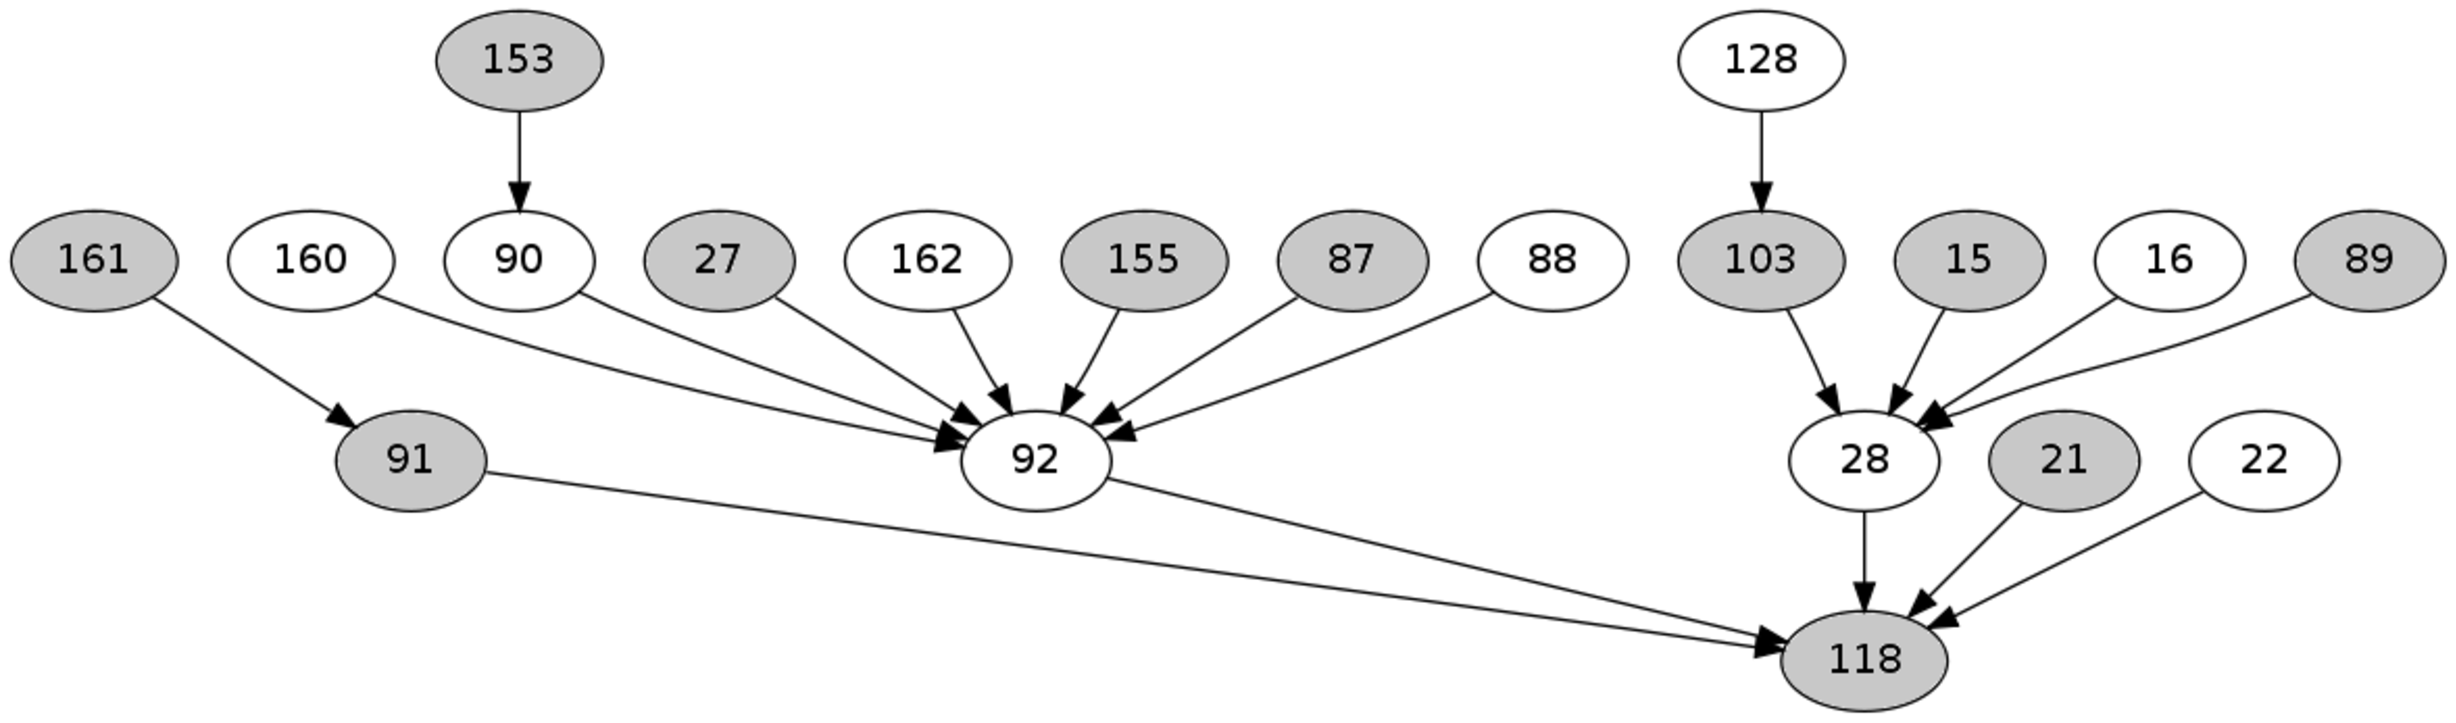
\includegraphics[width=0.7\hsize]{./5-idea/figs/ctp.pdf}\\
\textbf{(b)}\\
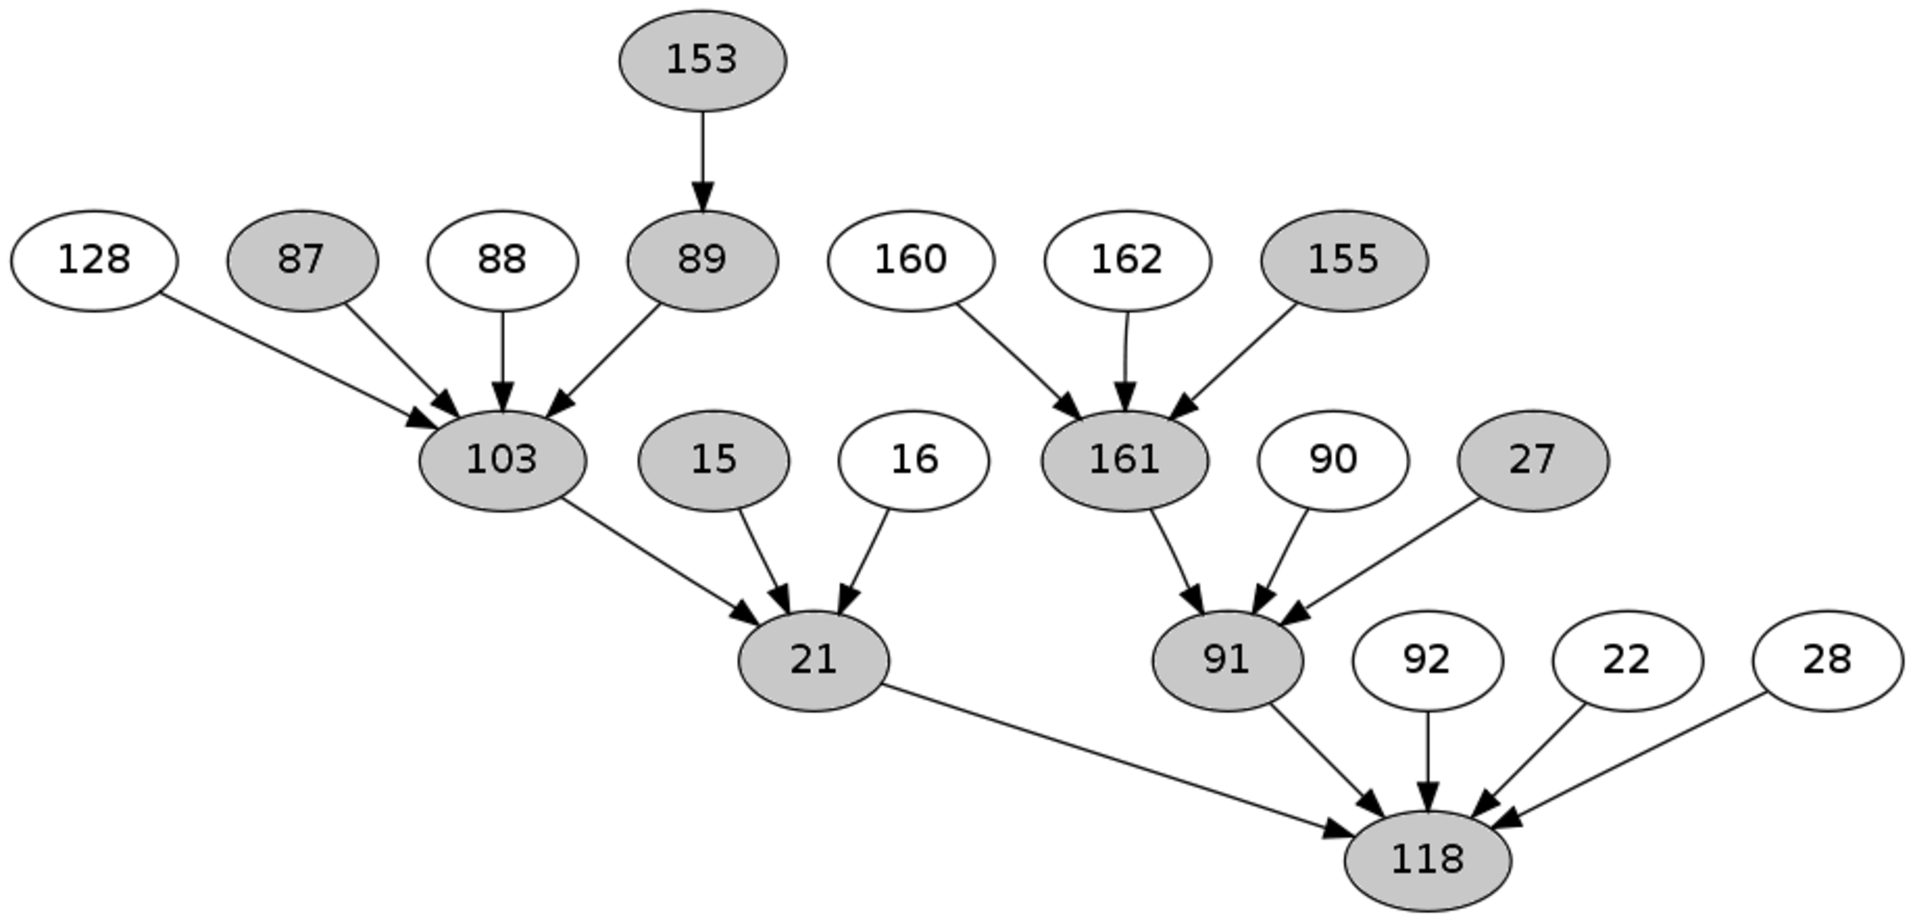
\includegraphics[width=0.7\hsize]{./5-idea/figs/ictp.pdf}\\
\end{center}

\caption{\textbf{Qualitative comparison of stock CTP and ICTP.} For this
experiment odd-numbered nodes (shaded) were set to charging rapidly, while
even-numbered nodes were not charging. Unmodified CTP builds the tree shown
in (a), which routes many packets through the even nodes. ICTP builds the
tree shown in (b), which moves all even nodes to leaf roles.}

\label{idea-fig-ictpqualitative}
\end{figure}

Using IDEA we were able to integrate energy awareness into CTP, the routing
protocol included as part of TinyOS. For these experiments each node in a
20~node network sends 6 packets to the sink per second. Static LPL intervals
of 0.5 second were used. 

Figure~\ref{idea-fig-ictpqualitative} shows a qualitative demonstration of
the difference between energy-aware and non-energy-aware routing trees. This
TOSSIM simulation ran with all odd numbered nodes charging rapidly and all
even numbered nodes not charging (with the exception of the powered sink,
Node 118). While this is an unrealistic charging pattern, it produces a clear
difference in routing protocol behavior.
Figure~\ref{idea-fig-ictpqualitative}(a) shows that unmodified CTP is unaware
of these charging differences and puts several even nodes, such as Node 92,
into positions where they are routing for multiple nodes. The total number of
nodes upstream from even numbered nodes in the stock CTP case is 14. In
contrast, ICTP realizes that the odd-numbered nodes have energy to spare and
the even-numbered nodes are lacking, and moves all even nodes to leaf roles.
None of the even nodes in Figure~\ref{idea-fig-ictpqualitative} are routing
data.

Using a 20~node subset of our MoteLab topology, we compared the performance
of ICTP to unmodified CTP using 24-hour TOSSIM simulations and the three
different solar charging scenarios previously described. As
Table~\ref{idea-table-ictpvoptimaltossim} shows, ICTP shows improvements in
lifetime over stock CTP of between 11 and 27\%. The different routing trees
formed by ICTP did not effect the packet delivery rates appreciably with the
largest change in packet delivery rate being 2.8\% (97.8\% for CTP vs. 95.0\%
for ICTP).

Finally, Table~\ref{idea-table-etxsearchradius} shows how IDEA can trade off
application utility with the energy objective function. The simulation
experiment uses a 25~node grid topology and, similar to the previous
experiment, half the nodes are charging rapidly while the other half are not.
Here our application-defined metric is expected transmissions to reach the
sink (ETX). A purely ETX-based tree will use the shortest route without
routing around the uncharging nodes, whereas an energy-aware tree will avoid
the uncharging nodes by constructing longer routes. We expect that,
prioritizing ETX will cause the total ETX of the entire tree --- defined as
the sum of the ETX of all the routes in use --- to decrease, while
prioritizing energy performance will cause the first-node lifetime of the
tree to increase.

Indeed, Table~\ref{idea-table-etxsearchradius} confirms this is the case. For
each experiment, we restrict the set of acceptable parents to be the minimum
available parent ETX plus an extra amount we call the ETX search margin. For
example, if the minimum available parent ETX is 5 and the ETX search margin
is 10, then we will consider all parents with ETX < 15. As the search margin
increases, IDEA will examine longer routes that may provide better energy
performance. As the table shows, increasing the ETX search margin leads to
longer average routes but also improves overall network lifetime.

\begin{table}[t]
\begin{center}
\begin{tabular}{|l|ccc|}
\hline
\textbf{Solar Charging} & \multicolumn{2}{c}{\textbf{Lifetime (hours)}} & \textbf{Increase} \\
\textbf{Pattern} & \textbf{CTP} & \textbf{ICTP} & \textbf{(\%)} \\ \hline
Large Panel & 17.1 & 19.0 & 11\% \\
Small Panel & 10.5 & 13.3 & 27\% \\
Random Attenuation & 10.5 & 12.2 & 16\% \\ \hline
\end{tabular}
\end{center}

\caption{\textbf{ICTP performance with solar charging.} The table summarizes
the performance improvements obtained by replacing CTP with ICTP. Three
different solar charging profiles are used: a large panel that completely
charges all batteries each day, a small panel that does not, and a randomly
attenuated charging profile that varies node-to-node.}

\label{idea-table-ictpvoptimaltossim}
\end{table}

\begin{table}[t]
\begin{center}
\begin{tabular}{|l|cc|}
\hline
\textbf{ETX Search} & \textbf{Total ETX} & \textbf{Network Lifetime} \\
\textbf{Margin (ETX)} & \textbf{(ETX)} & \textbf{(s)} \\ \hline
0 & 2442 & 4357 \\
10 & 2591 & 4737 \\
20 & 3207 & 5116 \\
50 & 3127 & 6216 \\
100 & 3442 & 6502 \\ \hline
\end{tabular}
\end{center}

\caption{\textbf{Tradeoff between energy-awareness and application utility.}
The results illustrate how IDEA can parameterize the tradeoff between
application-defined utility and the energy objective function.}

\label{idea-table-etxsearchradius}
\end{table}

\subsection{Distributed Localization}

To evaluate the distributed localization application we built a Python
simulator, which improves significantly on TOSSIM performance for hundreds of
nodes and allowed rapid iteration and experimentation with different energy
objective functions. Our simulator models acoustic event sources within the
sensor network, each of which triggers a distributed localization operation.
The energy overheads of communication, both the leader election process and
the subsequent data transfer, are modeled in the simulator based on empirical
measurements taken on our MoteLab testbed.

\begin{figure}[t]
\begin{center}
\includegraphics[width=\hsize]{./5-idea/figs/localizationdensityvtime.pdf}
\end{center}

\caption{\textbf{Energy density over time.} Energy densities for the
\texttt{Closest} heuristic and IDEA using the \texttt{WeightedEnergy}
objective function are shown at four points in time. The event distribution
is uniform. IDEA enables better load distribution, which leads to a longer
application lifetime.}

\label{idea-fig-localizationdensityvtime}
\end{figure}

For these experiments we arranged 100 nodes into a 100~m by 100~m area,
resulting in the placements shown in
Figure~\ref{idea-fig-localizationdensityvtime}. We simulate a sensing range
equal to the communication range, each set to 20~m. This radius is chosen to
give each node reasonable number of neighbors and allow it to detect a
reasonable number of events. We randomize the reliable transfer protocol
bandwidth across each link to between 768 and 1280~Bps, a feasible
range based on results from data transfer protocols such as
Flush~\cite{flush-sensys07} and Fetch. Events are simulated using a uniform
random distribution so that events have equal probability of occurring
anywhere in the sensor field.

To evaluate network performance, we define \textit{capability} of the network
as the percent of the last 100 operations that succeeded, where success is
defined as localizing the event. We assume that the application requires that
the network be able to be able to localize a high percentage of events that
occur, and design our energy objective functions with this in mind. As an
example, an intruder localization application is no longer useful once it
fails to detect a very high percentage of intrusion attempts. We quote the
system lifetime as the the 90\% capability time, the time at which the
network's capability drops below 90\%.

We experimented with several approaches to choosing a localization plan, one
that does not use IDEA and three that do using different energy objective
functions:

\begin{enumerate}

\item \textbf{\texttt{Closest}:} produces a localization plan with the node
closest to the event source as the aggregator and the three next closest
nodes as signal providers. We assume a real solution would use an imperfect
estimate of proximity such as total signal energy or signal-to-noise ratio,
but for the simulations we use the known simulated event location to choose
the closest nodes. \texttt{Closest} does not require energy state information
and so could be implemented without IDEA. It is implemented as an example of
a plausible non-energy-aware solution.

\item \textbf{\texttt{MaxEnergy}:} chooses the node with the most energy
(that heard the event) as aggregator and the next three highest-energy nodes
as signal providers.

\item \textbf{\texttt{TotalEnergy}:} chooses the localization plan that
consumes the lowest amount of total energy summed across all nodes in the
network.

\item \textbf{\texttt{WeightedEnergy}:} weights the total energy consumption
using a similarity metric derived from the cosine similarity index to measure
the degree to which the energy vector for the localization plan is a good
``fit'' given the current energy availability.

\end{enumerate}

\begin{figure}[t]
\begin{center}
\includegraphics[width=0.7\hsize]{./5-idea/figs/ideavheuristics.pdf}
\end{center}

\caption{\textbf{Performance of IDEA objective functions and heuristic.}
Simulation results are shown for the localization application. The graph
compares the \texttt{Closest} heuristic, implemented without using IDEA,
against three different IDEA objective functions: \texttt{MaxEnergy},
\texttt{TotalEnergy} and \texttt{WeightedEnergy}. The \texttt{WeightedEnergy}
approach using IDEA outperforms the non-energy-aware approach while the other
objective functions perform more poorly.}

\label{idea-fig-ideavheuristics}
\end{figure}

We began by experimenting with the \texttt{Closest}, \texttt{MaxEnergy} and
\texttt{TotalEnergy} approaches. As Figure~\ref{idea-fig-ideavheuristics}
shows, the \texttt{Closest} heuristic outperformed the two IDEA-based
approaches. However, when examining the energy density plot shown in
Figure~\ref{idea-fig-localizationdensityvtime} for the \texttt{Closest}
heuristic we could see that it led to concentrations of available energy on
nodes at dense locations on the irregular grid, while \texttt{MaxEnergy} did
a better job of exhausting all nodes simultaneously, as evidenced by the
extremely sharp drop in network capability it produces. This is despite the
uniform distribution of acoustic event sources, which one might expect to
produce good energy load distribution without the need for tuning.

Our analysis determined that the \texttt{MaxEnergy} suffers because it will
always route data through extra nodes in order to reach the node with the
most energy. So if that node is on the edge of the cluster of nodes that
heard the event, energy may be consumed by nodes within the interior in order
to allow the signal provides to communicate with the aggregator.
\texttt{MaxEnergy} leads to an even usage of energy across the network, but a
short lifetime, because it always prioritizes the distribution of energy over
the amount consumed when choosing how to localize each event.

In contrast, \texttt{Closest}, while it performs better, has the opposite
problem. While it does not consider energy directly, the effect of the
heuristic is to choose based on the total amount of energy consumed. By
selecting the nodes closest to the event, the heuristic almost always leads
to clusters where all signal providers can communicate with the aggregator,
so no extra energy expenditures by other nodes for routing are needed.
However, the non-uniform distribution of nodes means that some nodes more
likely to be the closest node than others, leading to unequal energy
distribution. While the lifetime is better than \texttt{MaxEnergy}, the
existence of energy at some nodes once the capability drops below 90\% led us
to believe that a hybrid approach was possible that would outperform both
\texttt{MaxEnergy} and \texttt{Closest}.

After exploring several additional approaches we found an energy objective
function capable of producing extremely good load distribution, the
\texttt{WeightedEnergy} approach described above.
Figure~\ref{idea-fig-ideavheuristics} shows that it outperforms
\texttt{Closest}, increasing the network's lifetime by 15\%, while
Figure~\ref{idea-fig-localizationdensityvtime} illustrates how it utilizes
all the nodes' available energy, achieving an even distribution similar to
\texttt{MaxEnergy}. It does this by combining aspects of both earlier
approaches. By weighing the total energy consumed it avoids the extremely
high-energy localization plans that the \texttt{MaxEnergy} function will
sometimes use. By also weighing the ``fit'' using the cosine similarity
metric we address unequal energy distribution in a way that the
\texttt{Closest} heuristic does not.

Our experience with the localization application illustrates the role of the
proper energy objective function in enabling good application performance,
and points to the increases in system lifetime possible through better energy
distribution. 

\section{Related Work}
\label{idea-sec-related}

Previous work has addressed the problem of energy load balancing in contexts
such as sensor coverage, role assignment, and energy-aware routing. Other
efforts in sensor networks have focused on reducing the power consumption at
individual nodes without considering energy distribution. Many of these
efforts are specific to a particular application or component and do not
provide a service like IDEA that can be used by a variety of applications. 

A number of existing systems such as Odyssey~\cite{odyssey-osr99},
PowerScope~\cite{powerscope-wmcsa99} and more recently
Cinder~\cite{cinder-mobiheld09}, have addressed measuring or adapting to
energy variations on battery-powered devices, primarily to support mobile
applications. This naturally produces a difference in approach from IDEA,
since IDEA targets networks consisting of multiple nodes but treated as a
single entity. Since nodes are collaborating we can enable more sharing and
ask nodes to sacrifice for each other, whereas mobile device users would
likely be upset if they discovered that their phone was running low on power
because it was trying to improve the lifetime of a stranger's phone located
nearby.

Quanto~\cite{quanto-osdi08} provides a framework for tracking and
understanding energy consumption in embedded sensor systems. The existence of
systems like Quanto was a primary motivation for IDEA, since the visibility
distributed resource tracking provides creates an opportunity to adapt to
changes in availability across the network. Currently IDEA requires that
components model their own energy consumption, which may be difficult for
components with complex behavior. We are exploring integrating Quanto into
IDEA to provide more precise tracking of energy at runtime, which could
eliminate the need for component-specific modeling and ease the process of
integrating applications with IDEA.

Eon~\cite{eon-sensys07} performs similar energy tracking and forward
projection but focuses on single-node, not network-wide adaptations.
SORA~\cite{sora-nsdi05} focuses on decentralized resource allocation based on
an economic model in which nodes respond to incentives to produce data or
perform specific tasks, with each node trying to maximize its profit for
taking a series of actions. While SORA, using correctly set prices, could
produce similar network-wide behavior to that enabled by IDEA, the connection
between prices and the behavior of the network is not completely clear. IDEA
simplifies the problem of global network control through the energy objective
function which directly expresses the application's goal.

Some work on energy-aware routing~\cite{ShahRabaey2002,381685} has addressed
equitable energy distribution within the network by probabilistically
choosing between multiple good paths between each source and sink pair.
LEACH~\cite{leach} and other similar approaches attempt to distributed energy
in an entirely decentralized way, using local heuristics to do so.

EnviroMic~\cite{enviromic} is a distributed acoustic storage system for
sensor networks. When EnviroMic nodes hear an acoustic event, a leader is
elected to assign recording tasks to nodes in the group. As storage space is
limited, EnviroMic attempts to push data to quiet sections of the network
with unused storage, balancing storage consumption across the network. Both
of these tasks involve choosing from a set of nodes that can perform the same
storage task, and so EnviroMic could be integrated with IDEA allowing the
energy overheads of data transfers to be considered.

The IDEA architecture emerged from our own prior work on energy management
for wireless sensor networks, including Lance~\cite{lance-sensys08},
Pixie~\cite{pixie-sensys08}, and Peloton~\cite{peloton-hotos09}. Lance
focused specifically on the problem of bulk data-transfer using resource
vectors and centralized control. By balancing the value and distributed cost
of retrieving sampled signals we enable near-optimal performance.  Pixie
proposed an operating system and programming framework for sensor network
nodes that promotes resources to a first-class primitive, using tickets to
manage resource consumption and brokers to enable specialized management
policies. Pixie does not consider the energy impact of a node on other nodes.

Peloton proposed an architecture for distributed resource management in
sensor networks combining state sharing, vector tickets to represent
distributed resource consumption and a decentralized architecture in which
nodes serve as ticket agents managing the resource consumption of themselves
and on behalf of nearby nodes. IDEA shares many features with Peloton and can
be viewed as the beginnings of an implementation of the Peloton design, with
state sharing to enable energy decision making and every node serving as a
ticket agent for itself but considering the distributed impact of its own
local state.


\chapter{Lessons Learned and Future Work}
\label{chapter-lessons}

This chapter summarizes some key observations and lessons that have emerged
from the work described in this dissertation. We describe a set of important
takeaways from our experiences deploying real systems, while also identifying
some strengths and weaknesses of two architectures described in the preceding
chapters. We also briefly outline areas for future work.

\section{Lessons Learned}

Broadly speaking, we can divide the takeaways mentioned here into two
categories. The first set relate to why and how to build applications and
perform field deployments. These have emerged from the process of building
and deploying three solutions in the context of the volcano monitoring
application. The second set comment on the strengths and weaknesses of the
two architectural solutions to sensor network resource management we have
presented: Lance and IDEA.

\subsection{Deployment Lessons}

Sensor network deployments, particularly in remote areas, involve significant
cost in terms of time and equipment. Failures of hardware and software can
have a negative impact on the uptake of this technology by domain science
experts. Our experiences at Ecuadorean volcanos have yielded a number of
valuable lessons for future sensor network deployments. 

\begin{itemize}

\item \textbf{Ground truth and self-validation mechanisms are critical.}
During our 2005 deployment, we did not initially consider colocating several
of our wireless sensors with existing data loggers in order to establish
ground truth. This would have clearly aided our analysis, though we were
fortunate to locate one of our sensors near (but not immediately adjacent to)
the RVEN station. In addition, self-validation mechanisms are needed to
provide detailed information on the health and accuracy of the data recorded
by the network. The periodic ``heartbeat'' messages that we built into our
system proved essential to remotely tracking system operation.

More generally, it is critical to design the evaluation process well before
the system being studied is designed and deployed. Deployments are expensive
and deployment time is valuable, and if the system is not properly
instrumented it can be difficult to assess its performance after the
deployment has ended.

\item \textbf{Coping with infrastructure and protocol failures.} As discussed
previously, in 2005 we were surprised to find that the sensor nodes
themselves were the most reliable components of the system. Even without
classifying the 3-day network outage as an infrastructure failure, this
downtime was far exceeded by outages caused by power failures at the base
station. We did not devote enough attention to assuring the reliability of
the base station and radio modem infrastructure, assuming it would be a
trivial matter of plugging into wall power. This single point of failure was
more fragile than expected.

Additionally, several pieces deployed software, including Deluge and FTSP,
exhibited failures in the field than we not had expected given our laboratory
experiments. These failures both speak for and show the limitations of
careful, pre-deployment testing. While we were fortunate to be able to
correct protocol errors in the field and during post-processing, the risk
of uncorrectable problems argues for more rigorous testing and analysis. At
the same time, the unpredictability of field deployments places demands on
the flexibility and adaptability of the researchers involved.

\item \textbf{Building confidence inside cross-domain scientific
collaborations.} It is important when working with domain scientists to
understand their expectations and plan carefully to meet them. There can be
tensions between the desire of computer science researchers to develop more
interesting, sophisticated and complex systems, and the needs of domain
science, which relies upon thoroughly validated instrumentation. Pushing more
complexity into the sensor network can improve lifetime and performance, but
the resulting system must be carefully validated before deployment to ensure
that the resulting data is scientifically accurate.

Good communication between computer and domain scientists is also critical.
During the 2005 deployment, the seismologists were eager to see the collected
signals, which were initially in an unprocessed format with timing errors as
described earlier. From the CS perspective, the early data provided evidence
of successful data collection, but from the geophysics perspective it
highlighted failures in the time synchronization protocol. It took a great
deal of effort after the deployment to build confidence in the validity of
our data.

Finally, the development of Lance required a great deal of exchange between
te domain and computer scientists involved. Seismologists are used to systems
able to provide complete, high-fidelity signals from all stations spanning
all time intervals. The capabilities of the instruments that they typically
deploy have meant that they have not had to think about how to classify data
once not all signals have been collected. Although they were initially quite
hesitant, we were able to convince them that the easy of deployment and
promise of increased spatial resolution provided by our low-power devices
made it worth abandoning complete temporal coverage. Once convinced, they
were very helpful in suggesting ways to prioritize collected signals and
suggested the node-level summarization functions used during the 2007
deployment.

\end{itemize}

\subsection{Architectural Lessons}

\begin{itemize}

\item \textbf{Balance centralization and decentralization.}

\item \textbf{Energy is the most important resource.}

\item \textbf{Treat the entire network as a single instrument.}

\item \textbf{Connect node-level behavior with application-level fidelity.}

\end{itemize}

\section{Future Work}

Despite advances in this area, sensor networks have just begun to make
inroads in augmenting and replacing existing scientific instrumentation. The
macroscope is still a new instrument, and requires much more research and
development before it can truly deliver the kind of views envisioned by de
Rosnay.

Opportunities remain for collaborations between sensor network researchers
and domain scientists in many areas. As described in
Chapter~\ref{chapter-related}, parallel efforts have already succeeded in
leveraging this technology to study animal habitats and behavior and a
variety of natural environments. Moving forward we expect to see these kinds
of scientific sensor networks defining an unique research agenda, with
emphasis on scaling out to thousands or millions of nodes, delivering large
amounts of high-fidelity data, and achieving perpetual operation predicated
on improved energy-harvesting capabilities.

These goals will continue to place pressure on key system capabilities
developed by the research described in this dissertation. Resources will
still be precious, and must be devoted to the most important information; and
energy availability will vary across the network in unpredictable ways,
potentially threatening high-fidelity operation.

The Lance architecture described in Chapter~\ref{chapter-lance} was broadened
and decentralized to produce IDEA, but several core challenges still remain.
Lance's linear policy modules are easy to use and compose, but it remains
unclear whether more complex interactions between policy modules are needed.
During the process of adapting Lance to support medical monitoring the policy
module architecture was revisted and extended, but incorporating additional
applications may require additional changes and more generality.
Additionally, Lance's reliance on a central controller limits the scalibility
of the architecture. While IDEA allows certain kinds of resource-management
decisions to be made in a distributed fashion, it does not completely
eliminate the need for complete network visibility when trying to optimize
certain tasks. Instead of aiming at a completely flat network, Lance may
adapt well to tiered systems that achieve scalability without moving nodes
too far away from devices with significant computational capabilities.

As far as IDEA, for future work we are interested in addressing the problem
of cross-component interaction which would allow us to optimize the operation
of several IDEA components running in the network simultaneously. This is
complicated by the fact that there is likely to be dependencies between
components that cause decisions made by one to affect others. As an example,
the LPL intervals used by a node would effect the power cost to use the link
seen by the routing protocol. Considering cross-component interaction also
rapidly expands the search space when nodes try to identify the right local
state to select. Currently we assume that the search space is small enough
that we can search it exhaustively. Cross-component support may require that
we develop more intelligent search strategies in order to allow this process
to be performed on computationally-constrained devices.

In addition we are investigating ways to model the impact of node failure on
other nodes. Many sensor network protocols will try to work around nodes
leaving the network or going offline, but this repair process is costly and
causes load within the network to shift in ways that are difficult to
anticipate \textit{a priori}. One option here is to use network-level
simulators running in parallel with the deployed system itself. Information
about the deployment environment can be harvested continuously to increase
the reality of the simulated outcomes. When trying to adjust network
behavior, the impact of various decisions could be evaluated quickly in
simulation incorporating the effect of node failures.


\chapter{Conclusion}
\label{chapter-conclusion}

While the last century was marked by a new understanding of our world at
microscopic scales, the next will be driven by holistic understanding of
large-scale systems. Wireless sensor networks composed of tens or hundreds of
low-power, resource-constrained devices, can aid scientific exploration by
providing high-fidelity data at scales more difficult to achieve with
traditional instrumentation. This dissertation has helped demonstrate the
promise of this new technology to enable the macroscope and macroscopic
science.

We began by describing how we tackled a single high data-rate scientific
application: volcano monitoring. Through a series of field deployments
working closely with seismologists, we acquired the domain knowledge
necessary to build a system meeting their needs. After a month-long
deployment at Reventador volcano in 2005, we performed a careful and detailed
analysis of our system's performance. Our study showed that wireless sensor
network technology was able to meet their data fidelity needs and pioneered a
new post-hoc time rectification protocol correcting protocol failures we
observed in the field.

\clearpage

After validating the core capability of our system to deliver data to the
scientists' specification, we addressed energy and bandwidth limitations with
a system called Lance. Lance optimizes reliable signal extraction by
considering both the energy cost and the value of the data to the
application, using a novel online heuristic to approach the performance of an
offline-optimal solution: within 5\% in most cases.

Next we addressed the problem of unequal energy distribution using a system
called IDEA. IDEA disseminates information about each node's current battery
and load rates and uses this to enable energy-aware operation. System
components can use the IDEA service to determine how their own local state
impacts the operation of the network as a whole, and use this feedback to
pick states that help improve application performance. We showed that IDEA
can improve the lifetime of the system by up to 27\%.

Both of these architectural solutions are steps forward for scientific sensor
networks, but more work is needed to fully enable the distributed sensor
macroscope. We hope that these efforts will help lead the way towards a full
realization of de Rosnay's vision and a better understanding of the world
around us.



% 11 Jan 2010 : GWA : Bibliography.

\ssp
\bibliography{thesis}

% 11 Jan 2010 : GWA : No appendices currently.
% \appendix
% \include{appendix}

\end{document}
